
%--------------------------------------------------------------------
% Document Style
%--------------------------------------------------------------------
% Save LaTeX kernel version of \@xfloat





\documentclass[12pt]{report}
\usepackage{smu_thesis}






\usepackage{epsf}
\usepackage{amsmath,bm}
\usepackage{graphicx}
\usepackage{verbatim}
\usepackage{algorithm}
\usepackage{algorithmic}
\usepackage{fancyhdr}

\usepackage{multirow}
\usepackage{url}

\usepackage[justification=centering]{caption} 

\usepackage{subfigure}
%\usepackage{subcaption}


\renewcommand{\algorithmicrequire}{\textbf{Input:}}
\renewcommand{\algorithmicensure}{\textbf{Output:}}
\renewcommand{\baselinestretch}{0.94}


\linespread{1.6}
%\thesisdraft

\begin{document}

%===================================================================
%   Change information used to create front pages of thesis
%===================================================================
%%
%%  last name, first name, initial
%%
 \Name{Cui}{Pengfei}{} %don't put anything in the last brackets

%%
%% title -- you have up to three lines to specify your title
%% each line should be no more than 48 characters long
%%
 \Title{Exploiting Spectrum Agility in Wireless Links and Networks}
       { }
       { }
%%
%% previous degress
%%
 \DegreeA{B.S., Beijing Institute of Technology, 2007}
 \DegreeB{M.S., University of Chinese Academy of Sciences, 2010}
%%
%% degree you are seeking
%%
 \DegreeSought{Doctor of Philosophy}
%%
%% major
%%
 \Major{Electrical Engineering}
 \University{Southern Methodist University}
 \School{Bobby B. Lyle School of Engineering}
%%
%% date the degree will be confered
%%
 \DegreeDate{TBA}
 \ThesisDate{TBA}
%%
%% is this a thesis, dissertation, or something else?
%%
 \ThesisType{Dissertation}
%%
%% your committee -- the rank of your advisor must be adjusted in
%% smu_thesis.sty if it is not Dr.
%%
 \Advisor{Joseph Camp}
 \CommitteeMemberA{Dr. Dinesh Rajan}
 \CommitteeMemberB{Dr. Eli Olinick}
 \CommitteeMemberC{Dr. Carlos Davila}
 \CommitteeMemberD{Dr. Panos Papamichalis}


%===================================================================
%   Create the front pages of the thesis
%===================================================================

 \ApprovalTitlePages

%%
%% include your acknowledgements
%% If no dedication, move Acknowledgement to where dedication is and add to
%% table of contents
%% \addcontentsline{toc}{chapter}{\protect \noindent {ACKNOWLEDGMENTS}}
 \begin{Acknowledgment}
 One of the great joys of completion is to look over the journey past and remember
all the friends and family who have helped and supported me along this long but 
fulfilling road. 

First and foremost, I would like to thank my advisor, Dr. Joseph Camp, who 
provided seemingly endless resources to support my work. I would also like to thank 
my co-advisor, Dr. Dinesh Rajan, who always provides great comments and suggestions on 
my research, presentations and publications. 
I could not have asked for better role models, each inspirational supportive, and patient.
They are not only my academic mentors but also model examples of 'American Dream' I can 
touch. 
I would not be where I am today without the time and effort you spent throughout my 
studies. 
Thanks also go to my other committee member, Dr. Panos Papamichalis, 
Dr. Carlos Davila, Dr. Eli Olinick, for providing novel perspectives to my work.

Special thanks to Dr. Joseph Cleveland, who offered several courses and always joined in 
our group discussion. Thanks to Buses By Bill Inc. and Bill Austin for their supports of 
our measurements system.

I am thankful for the collaborations and discussions within our research group, 
including Yongjiu Du, Jonathan Landon, Pengda Huang, Hui Liu, Jialin He, Matthew Tonnemacher, 
Eric Johnson, Yingsi Liang, Rita Enami, Bryan Jeon and Tiaotiao Wang. I am thankful for collaboration 
with Jialin He, Hui Liu, Jonathan Landon, Dr. Onur Altintas, Rama Vuyyuru, 
Yuanyuan Dong, Dr. Eli Olinick, Dr. Ehsan Aryafa, and Dr. Mung Chiang.

I would like to express my heartfelt gratitude to my wife, Yulin Wang. Without her love, 
support, patience and help, I would not overcome the hard times throughout my Ph.D studies.

I am indebted to my family, especially to my mother and father, for 
believing in me to complete this work.

Last, but not least, thanks to all people participate in our experiments.




 \end{Acknowledgment}

%%
%% include your abstract
%%
 \begin{Abstract}
 \begin{abstract} 

Vehicular wireless channels have a high degree of variability, presenting a
challenge for vehicles and infrastructure to remain connected. The emergence of
the white space bands for data usage enables increased flexibility for vehicular
networks with distinct propagation characteristics across frequency bands from
450 MHz to 6 GHz. Since wireless propagation largely depends on the environment
in operation, a historical understanding of the frequency bands' performance in
a given context, could speed multi-band selection as vehicles transition across
diverse scenarios.  In this paper, we leverage knowledge of in-situ operation
across frequency bands with real-time measurements of the activity level to 
select the optimal band for the particular application in use.  To do so, we
perform a number of experiments in typical vehicular topologies.  With a
model based on a Decision Tree and an in-situ training set, we can predict
the throughput on a free channel. 
We can then consider the activity level per band to compute the resulting performance 
one could expect on context information to guide protocol. In the field, we 
exploit the propagation differences experienced per band to show that training on a repeatable 
route can yield vast performance improvements from prior schemes.  We show that minimal  
amounts of training can provide such improvements and that a simple scheme that can allow
multiband adaptation gains when there is insufficient levels of training.


%Probably at this time we could not employ the bus doing the experiments.

%Unused spectrum whitespaces in the currently underutilized analog TV bands are able to exploit for future wireless networks. There are potential room for performance improvement of wireless communication in throughput, power consumption and link fairness extending wireless to these bands. Previous methods are focused on channel adaptation across multiple channels in one band without considering the propogation and other characters among different bands. In this work, we employ the propogation difference for performance prediction of multiband adaptation. To identify the crowded level,we involve an activity level of networks based on the statistics information during a time slot to make the prediction more accuracy. The amount of context information required for multiband adaptation and the influerence of window size for activity level are evaluated in this paper. We conduct indoor and in-field experiments to validate our method. The experimental results demonstrate that our method is able to achieve as ... 


\end{abstract}



 \end{Abstract}

 \PreliminaryPages

% Uncomment to insert a list of symbols from symbols.tex (or elsewhere)
 %\begin{listofsymbols}
 %\input{symbols}
 %\end{listofsymbols}

%%
%% include your dedication
%%
 \Dedicate{}

%===================================================================
%   Begin the body of the thesis
%===================================================================
\begin{thesis}
%===================================================================
%   Chapters are included here
%===================================================================

\chapter{Introduction} 
\label{ch:introduction}

Due to the ubiquity and convenience of wireless Internet service, the demand of 
wireless device users for efficient wireless links and networks are surging.
For example, wireless 
data traffic has increased for a thousand-fold over the last years and is 
expected to continue over the next decade~\cite{metis}, greatly motivating 
the improvement of wireless link communication and network deployment technology.

However, unlike wired networks, wireless devices share spectrum resources 
and have unstable, time-varying channel quality. For a vehicular
environment, the situation is even worse due to the frequently changing channel 
state. Drivers and passengers around the world could utilize a 
wide array of vehicular applications ranging from real-time traffic 
monitoring and safety applications to various infotainment applications.
However, the continuous use of such applications is limited due to the
challenge of transmitting over highly-dynamic vehicular wireless channels.
In such networks, the increasing availability of different frequency bands 
with correspondingly diverse propagation characteristics could allow flexibility 
and robustness of vehicular links. Even with spectral flexibility, links are 
extremely tenuous, demanding instantaneous decisions to remain connected, 
motivating an algorithm that can find the appropriate frequency band quickly 
and according to the current environmental context.

Clearly, more available spectrum is able to improve the performance for 
both links and networks. The FCC has approved the use of broadband 
services in the white spaces of UHF TV bands, which were formerly exclusively 
licensed to television broadcasters. These white space bands are now available 
for unlicensed public use, enabling the deployment of wireless access networks 
across a broad range of scenarios from sparse rural areas (one of the key 
applications identified by the FCC) to dense urban areas~\cite{carlson}. The 
white space bands operate in available channels from 54-806 MHz, having a far 
greater propagation range than WiFi bands for similar transmission power
~\cite{balanis2012antenna}. In WiFi and white space heterogeneous wireless 
network, the service area degree of an access point depends on the capacity 
of radios, the propagation range and the demands of the serving area. The scant 
frequencies of radios, the propagation distinctive and the demands diversity 
of population distribution bring the variation of an access point service area. 
These issues are substantial to designing an optimal network deployment and 
provide potential commercial wireless services to clients in any location.

White space frequencies is not only benefit the access tier network, 
but also provides opportunity for backhual tier networks. About a 
decade ago, numerous cities solicited proposals from network carriers 
for exclusive rights to deploy city-wide WiFi, spanning hundreds of 
square miles. While the vast majority of the resulting awarded 
contracts used a wireless mesh topology, initial field tests revealed 
that the actual WiFi propagation could not achieve the proposed mesh node
spacing. As a result, many network carriers opted to pay millions of 
dollars in penalties rather than face the exponentially-increasing
deployment costs (e.g., Houston~\cite{cnet_aug07} and Philadelphia
~\cite{arstechnica_may08}). Thus, while a few mesh networks have been 
deployed in certain communities~\cite{CRSK06,google_imc08}, wireless 
mesh networks have largely been unsuccessful in achieving the scale 
of what was once anticipated~\cite{taps}. Around the same time, the 
digital TV transition created more spectrum for use with data networks
~\cite{fccwhitespace}. These white space bands operate in available 
channels from 54-806 MHz, having increased propagation characteristics 
as compared to WiFi~\cite{balanis2012antenna}. Hence, the FCC has 
identified rural areas as a key application for white space networks 
since the reduced population from major metropolitan areas allows a 
greater service area per backhaul device without saturating wireless 
capacity. Naturally, the question arises for these rural communities 
as well as more dense urban settings: how can the emerging white space 
bands improve large-scale mesh network deployments?  While much work 
has been done on deploying multihop wireless networks with multiple 
channels and radios, the differences in propagation have not be 
exploited in their models~\cite{raniwala2004centralized,tang2005interference, si2010overview}, 
which could be the fundamental issue for the success of mesh networks 
going forward.

As white space frequencies are made available for wireless communication,
both the academic and  industry experts are seeking an integrated approach
for white space and WiFi bands in wireless links and networks. 
In this work, we seek to jointly use 
white space bands and WiFi bands in vehicular and large scale network deployments. 
We also
propose prospective graph theory solution for white space spectrum 
in short future. 


% Here

\section{Challenges}
% Challenges

Wireless links and networks suffer from the limited available resources
and interference. Everyone must 
share the bandwidth. Here, users and work carriers alike seek 
better service and lower cost for wireless networks. 
Spectrum agility offers a new promising resource to address these issues. 
%the spectrum agility, the diversity of spectrum and network 
%complexity have to be recognized prior to the solutions.

% VNC challenge
First, accurate knowledge of channel state is challenging to obtain due to the
time varying nature of channel quality and interference.
at the receiver. In recently, cognitive radio mechanisms which 
interleave channel accesses motivate the frequency band selection 
problem of finding the optimal spectrum on which to transmit
~\cite{ghasemi2008spectrum}. Prior work has considered a number of 
challenges in leveraging white space frequencies including spectrum 
sensing, frequency-agile operation, geolocation, solving stringent 
spectral mask requirements, and providing reliable service in unlicensed 
and dynamically changing spectrum~\cite{shellhammer2009technical}. In 
particular, there has recently been an acceleration in spectrum sensing 
work~\cite{rayanchu2011fluid, kim1996pulse,cabric2004implementation}. 
Based on these works, protocols have been built for multi-channel and/or 
multiband wireless operation~\cite{MOAR,raychaudhuri2003spectrum,sabharwal2007opportunistic}. 
Other works have presented methods for searching for the most efficient 
transmission channel~\cite{mo2005comparison}, discovering channel 
information~\cite{rayanchu2011fluid, sabharwal2007opportunistic}, and 
estimating channel quality~\cite{MOAR}. Moreover, the emergence of a 
number of diverse sensors on a vehicle motivates work on heterogeneous 
wireless networks, which have different frequency bands and technologies
~\cite{hossain2010vehicular}. Thus, the various communication standards 
have diverse throughput capacity, allowing the choice of technology 
to possibly usurp frequency band decisions. For example, an 802.11n 
link at 5.8 GHz with high levels of loss might still be a better choice 
than a Bluetooth link at 2.4 GHz with little loss due to the discrepancy 
of hundreds of Mbps in throughput capacity. While these works have 
considered spectral activity and developing protocols and algorithms to 
find spectral holes, less of a focus has been on coupling such information 
with historical performance in a given propagation environment.


% WINMEE
Second, in access layer network deployment, specific to rural areas, 
the lack of user density and corresponding traffic demand per unit area 
as compared to dense urban areas allows greater levels of spatial 
aggregation to reduce the total number of required access points, 
lowering network deployment costs. In densely populated urban areas, 
the greater concentration of users and higher levels of traffic demand 
can be served by maximizing the spatial reuse. While many works have 
worked to address multihop wireless network deployment in terms of 
maximizing served user demand and/or minimizing network costs, the 
unique propagation characteristics and the interference from coexisting
activities in white space bands have either not been jointly studied 
or assumed to have certain characteristics without explicit measurement
~\cite{si2010overview}. Specifically, previous work has investigated 
wireless network deployment in terms of gateway placement, channel 
assignment, and routing~\cite{he2008optimizing,marina2010topology}.
However, each of these works focus on the deployment in WiFi bands 
without considering the white space bands. Moreover, the assumption 
of idle channels held in these models fails to match the in-field 
spectrum utility, which could degrade the performance of a wireless 
network. These two issues are critical for designing an optimal 
network deployment and providing commercial wireless services to 
clients in any location.



% Whitecell
The larger propagation range of white space channels is able to adapt channel association of 
users located in large area. 
When the users distributed in a large area, the temporal diversity and spectral diversity become 
 key issues in white space wireless network applications. 
% Extreme cases and the middle of number of channels
In sparse rural areas, plenty of white space channels are able to deploy new white space network. 
However, in dense area, the number of  white space channels are restricted by FCC in a small number, 
such as there is none white space channel available in New York downtown~\cite{googlespectrum}. 
The carrier have deploy WiFi wireless networks in the dense area. 
Other than the plenty white space channels and none white space channel extreme cases, most areas 
of major cities in the United States have one to eight 
white space channels~\cite{googlespectrum}. 
These white space channels are able to complement the WiFi wireless networks to achieve better 
performance in coverage, power consumption, etc. Thus, exploiting these limited white space resource 
to improve the WiFi network in dense area is a perspective option for wireless networks. 
% Power saving, extreme cases
The white space frequencies offer not only more wireless capacity but also the convenience of access 
across large area for the heterogeneous wireless network structure. 
A single white space channel is able to satisfy all the users in the area when the total traffic demands of 
the users in the area are relatively low. The WiFi radios in the heterogeneous structure could be turned off 
for power saving. 
While when the total traffic demand of the users in the area is high, all the radios in the wireless network 
have to operate for the service of users.
However, the amount of traffic demands generally come across somewhere between these extremes. Thus, the 
question comes out, {\it in what degree the white space help to reduce the power consumptions of an existing 
WiFi mesh?} Especially when the WiFi mesh located in dense area with less white space channel availability.





% Whitemesh 
Moreover, in the backhual layer, researchers have done both centralized and 
distributed work for channel assignment and routing~\cite{raniwala2004centralized,wu2006distributed}.
However, the FCC's new policy bring new opportunities
and challenges for these issues.  Increased channel capacity and 
propagation diversity forces new consideration for existing solutions.
Since even the original multichannel problem has been proved to be NP-hard
which could not be solved in polynomial time, low complexity
solution for joint white space and WiFi usage is needed.
%the new white space application is an emergency for 
%both academy and industry. 
As shown in Google database~\cite{googledatabase}, 
the additional number of available white space frequency channels 
vary from city to city in US. Existing channel occupancy discussed in 
previous work~\cite{pcuiwinmee} has shown that the occupancy of 
frequency impacts on wireless network deployment. Naturally, the 
question arises for improving the performance as well as the optimization 
of utilization: {\it how can the emerging white space bands improve 
large-scale mesh network deployments?}  While much work has been done 
on deploying multihop wireless networks with multiple channels and 
radios, the differences in propagation have not been exploited in their 
models~\cite{tang2005interference, long2013fair,doraghinejad2014channel}, 
which could be {\it the} fundamental issue for the success of mesh 
networks going forward.

Moreover, the joint use of WiFi and white spaces  in 
access points depends on the capacity of radios, the propagation range 
and the demands of the service area. 
Thus, the new opportunities created by white spaces motivate the following 
questions for wireless Internet carriers, which have yet to be addressed: 
{\it (i) To what degree can white space bands reduce the network deployment 
cost of sparsely populated rural areas as opposed to comparable WiFi-only 
solutions?} and {\it (ii) To what degree can heterogeneous access points 
benefit the dense population areas and sparsely populated rural areas?}


% Contributions of previous work and future work plan
\section{Contributions}

This work proposes spectrum adaptation for both the wireless links and 
large scale network deployments to improve the performance of wireless devices in 
multiple frequency bands.

% Measurements
We perform indoor and in-field measurements in mutiple scenarios across Dallas-Fort Worth 
metroplex.
To do so, we use an off-the-shelf platform that allows direct comparison and 
simultaneous experimentation across four different wireless frequency bands 
from 450 MHz to 5.8 GHz with the same physical and media access layers. 
We first develop a framework for multiband adaptation using both historical 
information and instantaneous measurements. 
We perform in-field 
measurements of spectrum utilization in various representative scenarios 
across the DFW metroplex, ranging from sparse rural to dense urban areas 
and consider the environmental setting (e.g., downtown, residential, or 
university campus). 
We perform 24 hours in-field measurements in neighborhoods, campus, downtown business building, 
and urban business buildings. Through these in-field measurements, we estimate the achieved channel capacity of 
these typical area in north Texas.
We leverage the user mobility footprint through in-filed Android based WiEye measurements of Dallas area on weekdays. 




% VNC Contributions
For link adaptation, we develop multiband protocols 
which couple the prior knowledge of in-situ performance of various bands 
with the instantaneous knowledge of spectral activity, SNR, and the current 
location of each band to arrive at a decision for the optimal band on which to transmit. 
This framework is broad enough 
to study adaptation across licensed and unlicensed bands, including white 
space frequency bands. We propose two different machine-learning-based 
multiband adaptation algorithms. The first machine learning algorithm, 
referred to as the Location-based Look-up Algorithm, is based on the idea 
of $k$-nearest-neighbor classification. The second machine-learning-based 
algorithm uses decision trees for classification. For comparison, we also 
create two baseline adaptation algorithms which attempt to make the optimal
band selection based on only: (i.)~historical performance data, and (ii.)
~instantaneous SNR measurements across various bands. We perform extensive 
outdoor V-2-V experiments to evaluate the proposed algorithms. Our results 
indicate that the proposed machine learning based algorithms improve throughput 
by up to $49.3\%$ over these baseline methods.

% WINMEE
In the access layer network deployment, 
we perform a measurement study 
which considers the propagation characteristics and observed in-field 
spectrum availability of white space and WiFi channels to find the total 
number of access points required to serve a given user demand. 
Across 
varying population densities in representative rural and metropolitan 
areas, we compare the cost savings (defined in terms of number of access 
points reduced) when white space bands are not used. To do so, we first 
define the metric to quantify the spectrum utility in a given measurement 
location. With the in-field measured spectrum utility data in metropolitan 
and surrounding areas of Dallas-Fort Worth (DFW), we calculate the 
activity level in WiFi and white space bands. Second, we propose a 
measurement-driven framework to find the number of access points required 
for areas with differing population densities according to our measurement 
locations and census data. We then evaluate our measurement-driven framework, 
showing the band selection across downtown, residential and university 
settings in urban and rural areas and analyze the impact of white space 
and WiFi channel combinations on a wireless deployment in these 
representative scenarios. 
% Paper contributions
The main contributions of our work in this part are as follows: 
We develop a measurement-driven Multi-band Access 
Point Estimation (MAPE) framework to jointly leverage propagation and 
spectrum availability of white space and WiFi bands for wireless access 
networks across settings. We analyze our framework under capacity and 
coverage constraints to show that, with white space bands, the number 
of access points can be greatly reduced from WiFi-only deployments by 
up to 1650\% in rural areas. We quantify the impact of white space and 
WiFi channel combinations to understand the trade offs involved in choosing 
the optimal channel setting, given a certain number of available channels 
from multiple bands. Furthermore, we discuss to centralized using frequencies 
or distributed using them in single access point. Through our numerical 
simulation, we show that in dense area centralized using spectrum gain 
more than sparse area.
% MOA
For the heterogeneous access tier optimization, we perform a relaxed linear 
program which considers the variation of heterogeneous access point service 
area to find the lower bound total number of access points required to 
serve a given user demand. Further, we represent an Multiband Heterogeneous 
Access Point Deployment (MHAPD) greedy algorithm 
to approach the lower bound. Across varying white space and WiFi radios 
combination, population densities in representative rural and metropolitan 
areas we compare the cost savings (defined in terms of number of access 
points reduced) when white space bands are not used. We then evaluate our 
MHAPD algorithm, showing the heterogeneous band selection across downtown, 
residential and university settings in urban area and rural areas and analyze 
the impact of white space and WiFi combinations on a wireless deployment in 
these representative scenarios.
% Paper contributions
The main contributions of our work in this topic include: We develop an 
optimization framework based on linear programming to jointly leverage 
white space and WiFi bands approaching the lower bound in terms of the number 
of access points to serve the demands of a given area. We design a MHAPD 
greedy algorithm, which models the problem as a bin packing problem. We 
evaluate the performance of the presented algorithm, comparing with the 
lower bound and the hexagon of WiFi access point deployment in sparse rural 
areas given similar channel resources. The numeric results shows that our 
algorithm gains 260\% against the linear hexagon of deployments.  We 
further analyze the performance of heterogeneous access point performance 
across variety of population densities. The numeric results show that heterogeneous 
access points which jointly use white space and WiFi bands could improve 
the budget saving up to 323\%. 

% Whitecell
% Work summary 
In the white space power consumption analysis, we study the white space resource impacts on 
mesh network power consumption via queuing theory model.
We describe the heterogeneous wireless network structure with both white space bands and WiFi bands. 
We formulate the system as a queuing model. We analyze the heterogeneous structure under the the waiting 
time constraint for resource allocation in multiple scenarios of the structure. We further propose a Greedy 
Server-side Replace (GSR) algorithm to minimize the power consumption for the heterogeneous network structure. 
We then evaluate the algorithm, showing the power consumption gains across sparse and dense areas and 
analyze the impact of the number of white space and WiFi channels in these representative scenarios.
% On demand consideration
% Paper contributions
Through the measurements analysis, we tell the user distribution in multiple types of areas across 24 hours in weekdays. 
We formulate the heterogeneous wireless structure as a queuing system. Based on previous queuing theory works, we 
analyze the resource allocation of the system quality of service in waiting time. Based on the analysis, we propose a 
Greedy Server-side Replace (GSR) algorithm to allocate the channel resource to minimize the power consumption.
We perform measurement-driven numerical simulations to analyze various scenarios of channel resource and 
users distribution. Our results shows that the white space bands reduce the power consumption in
sparse area by up to 512.55\% in weekdays.


% Whitemesh
In the backhual layer network deployment, we leverage the diversity 
in propagation of white space and WiFi bands in the planning and deployment
of large-scale wireless mesh networks. To do so, we first form an 
integer linear program to jointly exploit white space and WiFi bands 
for optimal WhiteMesh topologies. Second, since similar problem 
formulations have been proved to be NP-hard~\cite{jain2005impact}, 
we design a measurement driven heuristic algorithm, Band-based Path 
Selection (BPS). We then apply the approaching method in multiple 
scenarios with in-field measurement data. Across a wide range of 
scenarios, including network size, population distribution, deployment 
distance gap, we exploit when and  how to emerge white space 
bands in mesh networks. The performance of our scheme is compared 
against two well-known multi-channel, multi-radio channel assignment 
algorithms across these scenarios, including those typical for rural 
areas as well as urban settings. We further discuss how the channel occupancy 
impacts on wireless networks and show the comparison of our algorithm 
and previous methods in typical scenarios. Finally, we quantify the degree 
to which the joint use of both band types can improve the performance of 
wireless mesh networks. We analyze the white space bands application in 
wireless network deployment and develop an optimization framework based 
on integer linear programming to jointly leverage white space and WiFi 
bands to advantages and disadvantages in wireless mesh networks with measured
channel occupancy. We build a heuristic measurement driven algorithm, 
Band-based Path Selection (BPS), which considers the diverse propagation, 
overall interference level of WiFi and white space bands with measurement 
adjust. We perform extensive analysis across offered loads, network sizes, 
mesh nodes spacing and WiFi/white space band combinations, to compare 
against previous multichannel multiradio algorithms. 
We discuss the channel occupancy and mesh spacing impacts the 
performance of similar channel resources (bandwidth and transmission 
power), We show the improvement of our BPS algorithm in typical configurations up to 
180\% versus. previous multichannel algorithms.



% Future work
In the future, we propose to find a better solution based on graph
theory for multiband wireless network deployments. Future work will
provide a mechanism for not only channel assignment, but also where 
we should locate 
the gateway nodes with a less complex solution to achieve a 
complete framework for multiband wireless network deployment. 
%Also 
%we are interested in involving beamforming to increase the spatial
%reuse in wireless network with more capacity and fairness. 
%In the beamforming application, we are going to design protocols to 
%optimize the network deployment cost under the limitation of QoS.
%
% Beamforming network time? maybe could be a concept similar to network efficiency


% Thesis Overview
\section{Thesis Overview}

In Chapter~\ref{ch:background}, we discuss the background of this work, 
including the basic knowledge related to this work and the hardware 
platform and software tools applied in our research. 
Chapter~\ref{ch:measurements} introduce our indoor and in-field measurements in 
Dallas-Forth Worth metroplex.
Chapter~\ref{ch:vnc} 
provides an analysis and solution of vehicular link adaptation across multiple frequency bands. 
We also propose an access network deployment 
framework in Chapter~\ref{ch:winmee} and discuss the optimization of a 
single access point with spectrum limitations. Then, we further
compare this solution to one which both white space bands and WiFi 
bands to quantify the benefit of white spaces. In Chapter~\ref{ch:wm}, we propose an 
algorithm to assign channels in multiband wireless network scenarios for 
optimizing the throughput performance in multihop backhual networks. Further, we 
quantify the heterogeneous application of white space bands and WiFi bands 
in access points deployment process. 
%In Chapter~\ref{ch:futurework}, we 
%propose the future in multiband network deployment using graph theory for locating
%gateway nodes. 
Finally, we conclude our work and propose future plan in Chapter~\ref{ch:conclusion}.


\chapter{Background} 
\label{ch:background}

In this chapter, we describe the background of our research, 
including the basic technology related to this work, the 
hardware and software tools that we used to implement and evaluate 
our proposed algorithms in this work.


\section{White Space Bands}

The white space band term is mentioned the frequencies channels 
previously used by analog TV broadcasts. In United States, full 
power analog television broadcasts, which operated between the 
54 MHz and 806 MHz television frequencies (Channels 2-69), ceased 
operating on June 12, 2009 per a United States digital switchover 
mandate. At that time, full power TV stations were required to 
switch to digital transmission and operate only between 54 MHz 
and 698 MHz.~\cite{fccwhitespace} 

Industry and academia have recognized the value of white space 
bands in wireless communication. Various proposals, including 
IEEE 802.11af, IEEE 802.22 and those from the White Spaces 
Coalition, have advocated using white spaces left by the termination 
of analog TV to provide wireless broadband Internet access. Some 
company from industry has designed device intended to use these 
new available channels as a "white-spaces device" (WSD), such as 
Ubiquiti SR serials products. These devices are designed to detect 
the presence of existing but unused areas of airwaves, such as 
those reserved for analog television, and utilize these unused 
airwaves to transmit signals for data traffic. Such technology 
is predicted to improve the availability of broadband Internet 
service, especially in rural areas.

White space bands and ISM WiFi bands have great variation of 
propagation characteristics. Wireless propagation refers to 
the signal loss characteristics when wireless signals are 
transmitted through the wireless medium. The strength of the 
received signal depends on both the line-of-sight path (or lack 
thereof) and multiple other paths that result from reflection, 
diffraction, and scattering from obstacles~\cite{andersen1995propagation}. 
The widely-used Friis equation characterizes the received signal 
power $P_r$ in terms of transmit power $P_t$, transmitter gain 
$G_t$, receiver gain $G_r$, wavelength $\lambda$ of the carrier 
frequency, distance $R$ from transmitter to receiver, and path 
loss exponent $n$ according to~\cite{friis}:

\begin{equation}
\label{eq:friis}
P_r=P_t+G_t+G_r+10n \log_{10}\left( \frac{\lambda}{4\pi R}\right)
\end{equation}
Here, $n$ varies according to the aforementioned environmental 
factors with a value ranging from two to five in typical outdoor 
settings~\cite{rappaport}.

According to Eq.~\ref{eq:friis} white space band not only provide more 
bandwidth for wireless communication, but also bring the diversity in 
transmission/interference range. Our algorithms and frameworks try to 
exploit white space bands advantages of link communication and network 
deployment through spectrum agility with WiFi bands.


\section{Spectrum Utilization}

When access a channel licensed by FCC, most of the time we could detect signals in the 
air from devices who share the channel. To represent the utilization level of a channel, 
we define \emph{activity level}, $A$, as the percentage of time when the channel is 
occupied by all competing sources $x_j (j = 1, 2, 3, ...)$ other than the intended 
transmitter $y$. For 802.11-based transmissions, the activity level on band $i$ is 
defined as:
\begin{equation}
\label{eqn:80211activity}
A^i = \frac{\sum_j{\sum_k{\frac{L_k^{x_j}}{R_k^{x_j}}}}}{\sum_k{\frac{L_k^y}{R_k^y}}+\sum_j{\sum_k{\frac{L_k^{x_j}}{R_k^{x_j}}}}+S\sigma}
\end{equation}
where $L_k^{x_j}$ and $R_k^{x_j}$ represent the packet length in bits and data
rate at which that packet is transmitted, for external sources $x_j$;
$S$ and $\sigma$ are the number of idle slots and slot duration, respectively. 
When considering the activity level of non-802.11 users 
({\it e.g.}, the bands currently licensed to TV),
we use the received signal level from non-802.11 interfering sources $P_N^i$ 
on band $i$ directly as an input to our algorithms. 


% Talk about the available channel
In practical, we get the activity level through in-field measurements.
The measurements process will be introduced in following chapters.
We define the percentage of sensing samples ($S_\theta$) above an 
interference threshold ($\theta$) over the total samples ($S$) in a time unit as the 
activity level ($A$) of inter-network interference:
\begin{equation}
\label{eq:actdef}
A=\frac{S_\theta}{S_a}
\end{equation}
The capacity of a clean channel is denoted by $C$. With the protocol model, the capacity 
of a channel with inter-network interference $C_r$ could be represented as 
the remaining free time of the channel capacity according to: 
\begin{equation}
\label{eq:intercap}
C_r=C*(1-\bar{A})
\end{equation}


% WiEye Measurements
\section{WiEye Measurement Platform}
% WiEye introduction
WiEye application created for the data collection is currently available for download and usage via the Google Android 
Market under the name WiEye. The application offers WiFi access points connection quality in both graphical and tabular 
form. All data collection is done in the background, either continuously while the user is running the application or 
periodically if the user has opted in to background data collection to SMU research. 
The data collected has been approved by the Southern Methodist University Institutional Review Board, a human subjects 
research committee,ensuring that all ethical precautions have been taken in collecting data from the users of our 
application.

% FIXME need figures





\section{Gateworks Platform}

The off the shelf platform we use for our measurements is the GW2358. 
GW2358 is a member of the Gateworks Cambria Single Board Computer family. 
The GW2358 meets the requirements for enterprise and residential network 
applications. This single board computer consists of an Intel IXP435 XScale 
operating at 667MHz, 128Mbytes of DDRII-400 DRAM, and 32Mbytes of Flash. 
Peripherals include four Type III Mini-PCI sockets, two 10/100 Base-TX 
Ethernet ports with IEC-6100-4 ESD and EFT protection, two USB Host ports, 
and Compact Flash socket. Additional features include digital I/O, serial 
EEPROM, real time clock with battery backup, system monitor to track 
operating temperature and input voltage, RS232 serial port for management 
and debug, and watchdog timer. The GW2358 also supports GPS and RS485 
serial port as ordering options. Power is applied through a dedicated 
connector or through either Ethernet connector with the unused signal 
pairs in a passive power over Ethernet architecture. 
An open source software OpenWrt board support package is included 
for Linux operating systems.


\begin{figure} 
%\vspace{-0.1in}
\centering
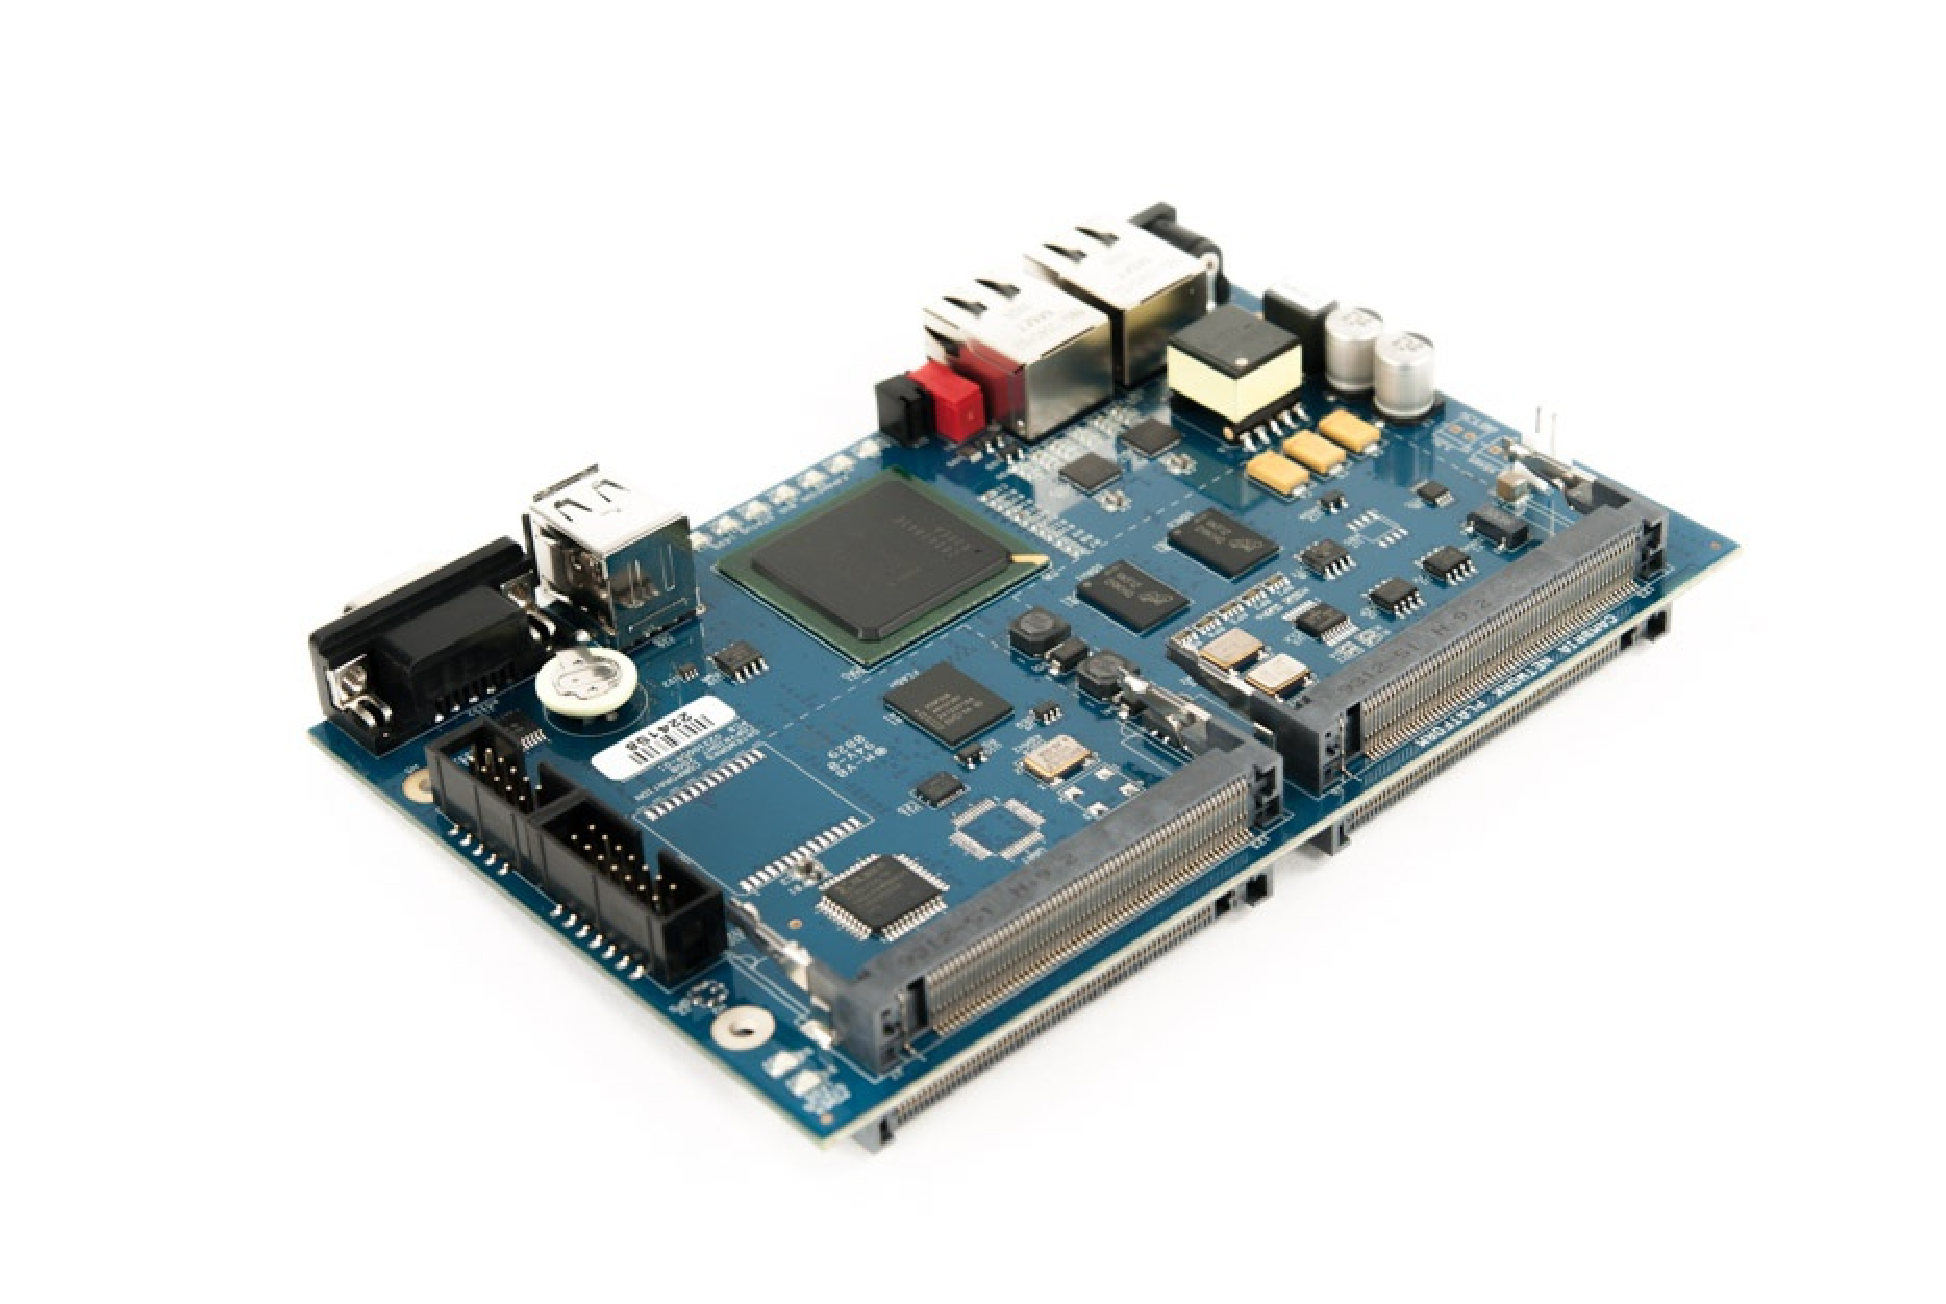
\includegraphics[width=75mm]{figures/gw2358}
\vspace{-0.1in}
\caption{The Gateworks GW2358 off-shelf Platform.}
\label{fig:gw2358}
\vspace{0.1in}
\end{figure}



The Gateworks platform works with Ubnt radios to perform 802.11 
multiband measurements for both indoor and in-field. It helps to 
collect the SNR, throughput and packet information for the post 
process. 

\section{Rohde \& Schwarz FSH8 Spectrum Analyzer}

The R\&S FSH 8 spectrum analyzer is designed portable for application 
in multiple environment, especially for in-field measurement. Its low 
weight, its simple, well-conceived operation concept and the large number 
of measurement functions make it an indispensable tool for anyone who 
needs an efficient measuring instrument for outdoor work. We employ 
FSH 8 in our indoor and outdoor measurements to collect data in multiple
bands.

\begin{figure} 
%\vspace{-0.1in}
\centering
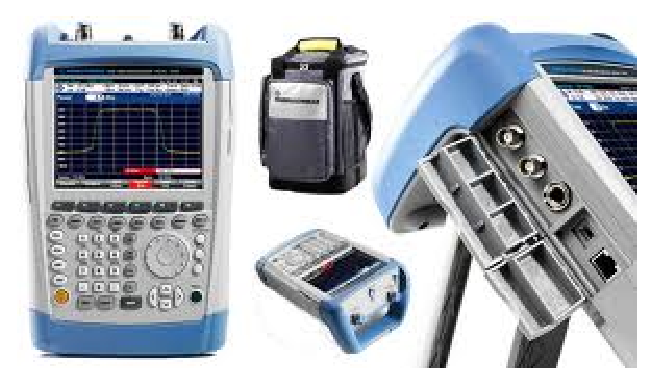
\includegraphics[width=75mm]{figures/fsh8}
\vspace{-0.1in}
\caption{Rohde \& Schwarz FSH 8 Spectrum Analyzer.}
\label{fig:fsh8}
\vspace{0.1in}
\end{figure}

FSH 8 is able to sense the signal in the air from 9 KHz to 
8 GHz. The spectrum analyzer could sense both 802.11 signals 
and non-802.11 signal in the air. Through the time stamp, 
we could merge data from Gateworks platform and FSH8 platform 
to perform our algorithms and frameworks.

\section{Mesh Network Deployment}

A wireless mesh network is a common infrastructure for providing 
wireless access for clients by the network carriers. Wireless 
mesh networks is made up of multiple radios which organize in a mesh 
topology. Each node forwards messages on behalf of the 
other nodes. The nodes connected to clients are referred to as the 
access tier. The nodes to relay data traffic to 
wired networks are referred to as the backhual tier. For the  access tier, the 
nodes need to cover the service area and provide sufficient 
capacity for the clients in target area. The backhual 
tier needs to have a highly-efficient path to the wired 
network which can potentially shorten multiple wireless hops. 
We analyze mesh network deployments in a scenario which includes multiple frequency bands, 
and propose our solutions for access and backhual 
network deployment.


\chapter{In-field Measurements} 
\label{ch:measurements}

In this chapter, we describe the background of our research, 
including the basic technology related to this work, the 
hardware and software tools that we used to implement and evaluate 
our proposed algorithms in this work.


\section{White Space Bands}



\chapter{Vehicular Link Spectrum Adaptation} 
\label{ch:vnc}

%
\section{Introduction}
\label{sec:introduction}


%Background
%Worldwide governments and societies are active to achieve road safety and travel comfort of drivers and passengers.
Drivers and passengers around the world could utilize a wide array of vehicular applications ranging from real-time traffic monitoring and
safety applications to various {\it infotainment} applications.
%spanning news, weather, audio, and video streams.  
However, the continuous use of such applications is limited due to the challenge of transmitting over 
highly-dynamic vehicular wireless channels. 
In such networks, the increasing availability of different 
frequency bands with correspondingly diverse propagation characteristics could allow flexibility and 
robustness of vehicular links. Even with spectral flexibility, links are extremely tenuous, 
demanding instantaneous decisions to remain connected, motivating an algorithm that
can find the appropriate frequency band quickly and according to the current environmental context.

Cognitive radio mechanisms which interleave channel accesses also motivate the frequency
band selection problem of finding the optimal spectrum on which to 
transmit~\cite{ghasemi2008spectrum}.
%Furthermore, in existing systems, there are a number of different technologies from which to choose and the demand of
% integrating the advantages of multiple protocol is presented as Heterogeneous Wireless Networks has opening topics related to band selection~\cite{hossain2010vehicular}.
Prior work has considered a number of challenges in
leveraging white space frequencies including spectrum sensing, frequency-agile operation,
geolocation, solving stringent spectral mask requirements, and providing reliable service
in unlicensed and dynamically changing spectrum~\cite{shellhammer2009technical}. In particular, there has recently been an acceleration
in spectrum sensing work~\cite{rayanchu2011fluid, kim1996pulse,cabric2004implementation}. Based on 
these works, protocols have been built for multi-channel and/or multiband wireless operation~\cite{MOAR,
raychaudhuri2003spectrum,sabharwal2007opportunistic}.  Other works have presented methods for searching for the most efficient 
transmission channel~\cite{mo2005comparison}, discovering channel information~\cite{rayanchu2011fluid, sabharwal2007opportunistic}, and estimating 
channel quality~\cite{MOAR}.
Finally, the emergence of a number of diverse sensors on a vehicle motivates work
on heterogeneous wireless networks, which have different frequency bands {\it and}
technologies~\cite{hossain2010vehicular}. Thus, the various communication 
standards have diverse throughput capacity, allowing the choice of technology 
to possibly usurp frequency band decisions. For example, an 802.11n link at 5.8 
GHz with high levels of loss
might still be a better choice than a Bluetooth link at 2.4 GHz with little loss
due to the discrepancy of hundreds of Mbps in throughput capacity.
%To consider the choice of frequency band, band selection problem for htereogeneous wireless networks should be researched under the same protocol, which make it similar to our problem~\cite{hossain2010vehicular}.
%Add heterogeneous and cognitive radio
%Research of heterogeneous wireless networks has been done for these purpose in Roadside-to-Vehicle and Vehicle-to-Vehicle.\cite{hossain2010vehicular}.
%the understanding of primary/secondary users adaptation\cite{cordeiro2007c}, combining multiple devices for vehicle~\cite{hossain2010vehicular}.

However, for the purposes of this work, we assume the underlying technology is the same to evaluate the choice of frequency band.
While these works have considered spectral activity and developing protocols and algorithms to 
find spectral holes, less of a focus has been on coupling such information with historical performance in a given 
propagation environment.
In this paper, 
we develop multiband adaptation protocols which couple the prior knowledge of in-situ performance of various bands with the instantaneous knowledge of 
spectral activity, SNR, and current location of each band to arrive at a decision on the optimal band to transmit. To do so, we use an
off-the-shelf platform that allows direct comparison and simultaneous experimentation across four different wireless
frequency bands from 450 MHz to 5.8 GHz with the same physical
and media access layers. 
%changes that frequency differences of hundreds of MHz to GHz could have on the band %decision. Moreover, it is well known that propagation greatly depends on the environment %in operation~\cite{rappaport}.  Thus, knowledge of the environment in operation could %allow the relationship between received power differences across multiple frequency bands %to have much greater accuracy.  

%Contributions  fixme
The main contributions of our work are as follows:
\begin{itemize}
\item We first develop a framework for multiband adaptation using both historical information and instantaneous measurements. This framework is broad enough to study adaptation across licensed and unlicensed bands, including white space frequency bands.  

\item We propose two different machine-learning-based multiband adaptation algorithms. The 
first machine learning algorithm, referred to as the \emph{Location-based 
Look-up Algorithm}, 
is based on the idea of $k$-nearest-neighbor classification. The second machine-learning-based 
algorithm uses \emph{decision trees} for classification. 
For comparison, we also create two baseline adaptation algorithms which attempt to make the optimal band selection based on only: (i.)~historical 
performance data, and (ii.)~instantaneous SNR measurements across 
various bands. 

%We consider four different algorithms for comparison.  First, we consider a scheme
%in which the throughput is achieved on an emulated channel for
%the current received signal level. We then adjust the predicted best band choice according to the current activity
%level (real-time information). 
%Second, we consider an approach based on machine learning which
%considers prior throughput for a given received signal and activity level
%combination.  
%Third, we build a scheme which include the prior relationship of throughput, received signal level and context information in an look up table for repeatable travel in an area.
%Fourth, we split the area to different regions and apply machine learning in each region to get the property band selection.

%earning in addition to the received signal and activity level.
%Third, we consider a second machine learning approach which considers user
%location in addition to the received signal and activity level.

\item We perform extensive outdoor V-2-V experiments to evaluate the proposed algorithms.
Our results indicate that the proposed machine learning based algorithms improve
throughput by up to $49.3\%$ over these baseline methods.

\end{itemize}



%The remainder of this paper is organized as follows. In Section II, we present the multiband adaptation problem and proposed algorithms. Section III discusses experimental evaluation of the multiband algorithms. We conclude in Section IV.




In this section, we first formulate the multiband 
adaptation problem in vehicular wireless links and introduce the set of information we use to make band decisions, which we refer to as context information. We then propose two machine-learning-based 
multiband adaptation algorithms for vehicular channels. For comparison, we also propose two baseline adaptation methods based on existing solutions which consider historical and instantaneous information independently.




\section{Link Adaptation Problem Formulation}
%The focus of this paper is on a context-based multiband adaptation algorithm as:
%The problem we are going to resolve is to find a band has the best throughput in multiple available options as:

Consider a system with~$n$ frequency bands, represented by an index set~$\{1,2, \ldots, n\}$. 
The objective is to select the optimal band,~$b_{best}$, to transmit at each time instant that maximizes a desired objective function such as throughput. The throughput~$r_i$ on band~$i$ depends on several factors such as received signal power~$P_R^i$, noise power~$P_N^i$, the channel activity level~$A^i$, the velocity of the transmitter,~$v_{tx}$,
 the velocity of the receiver,~$v_{rx}$, 
 and location information which depends on each algorithm and will be specified in the algorithm section. The aforementioned set of all information used to make multiband decisions composes the users context. 
 %Add Context
% Context is the information that can represent the characters of a wireless user.For mobile wireless users, velocity, RSSI, interference and location could be counted as context information.
This relationship is represented in general as~$r_i = f(P_R^i, P_N^i, A^i, v_{tx}, v_{rx}, $context information per algorithm$)$. The objective can be stated as:
\begin{equation}
b_{best}= \arg \max_i r_i 
\end{equation}
The framework differentiates interference from other nodes using the same technology (via the Activity level $A^i$) and other technologies (via the noise level~$P_N^i$). For instance, an 802.11 node can decode the packets of other 802.11 nodes but can only sense
instantaneous noise levels from ZigBee/Bluetooth nodes. 
Decoding the packets can provide increased knowledge such as 
data rate and packet size to determine the duration of the channel use.
%To help make decisions for multiband adaptation in a similar context,
We can exploit the long-term behavior by using historical performance
data for the collected context information
({\it e.g.}, $v_{tx}$, $v_{rx}$, $A^i$, $P_N^i$, $P_R^i$)~\cite{meikle2012global}. 
%can be used by people tending to have repeatable patterns
%~\cite{meikle2012global} and we could improve the performance with each trip 
%to the region if we could passively observe context along this repeatable 
%pattern. The variables used in each algorithm will be explained for each algorithm 
%later. 


%To represent the utilization level of the channel, we define \emph{activity level}, $A$,
%as the percentage of time when the channel is occupied by 
%all competing sources $x_j (j = 1, 2, 3, ...)$ other than the intended transmitter $y$. 
%For 802.11-based transmissions, the activity level on band $i$ is defined as:
%\begin{equation}
%\label{eqn:80211activity}
%A^i = \frac{\sum_j{\sum_k{\frac{L_k^{x_j}}{R_k^{x_j}}}}}{\sum_k{\frac{L_k^y}{R_k^y}}+\sum_j{\sum_k{\frac{L_k^{x_j}}{R_k^{x_j}}}}+S\sigma}
%\end{equation}
%where $L_k^{x_j}$ and $R_k^{x_j}$ represent the packet length in bits and data
%rate at which that packet is transmitted, for external sources $x_j$;
%$S$ and $\sigma$ are the number of idle slots and slot duration, respectively. 
%When considering the activity level of non-802.11 users 
%({\it e.g.}, the bands currently licensed to TV),
%we use the received signal level from non-802.11 interfering sources $P_N^i$ 
%on band $i$ directly as an input to our algorithms. 

\section{Multiband Adaptation Algorithms}
\label{subsec:algorithms}

In order to evaluate the proposed multiband adaptation algorithms, 
we construct two baseline methods: (i.) We search for the
most commonly selected band as the best band in the historical data
and choose it as the final band decision. (ii.) For each band, we build 
a lookup table for throughput $T_{ideal}$ in an idealized channel given the $RSSI$ and obtain 
the best band according to following:
\begin{align}
&\max_i\ T_{ideal}^i\times(1-A^i),
\label{eq:baseline2}
\end{align}
The throughput $T_{ideal}$ is measured with an Azimuth ACE-MX channel emulator~\cite{AzimuthACE}. 
The details of the system setup and data collection are discussed in Section~\ref{sec:vncexperimentdesign}. 

Machine learning has been used as an important tool in wireless communications~\cite{haykin2005cognitive}. When a user enters an area, the machine
learning algorithm can learn from the historical data and
select the potential optimal band given the input, {\it e.g.}, $P_R^i$, $v$
and $P_N^i$. We propose two multiband adaptation algorithms based on
two machine learning methods: k-nearest neighbor (KNN) and decision trees.

%2 machine learning methods: 
%1. modified KNN, 

{\bf Location-based Look-up Algorithm.} KNN is a machine learning method
based on searching for the closest training data points in the feature space and various
modified versions have been applied successfully for classification~\cite{zhang2006svm}.
In the {\it Location-based Look-up Algorithm}, we search for the closest neighbors of 
a testing point by using each parameter one by one in the input set. 
The {\it Location-based Look-up Algorithm} additionally involves geographic information for band selection other than received signal power~$P_R^i$, noise power~$P_N^i$, the activity/occupancy level~$A^i$, the velocity of the transmitter,~$v_{tx}$.
The 
performance of the selected training data points is averaged to generate an estimate of the performance at each band. Then
the band with the highest throughput performance is selected as $b_{best}$.
%comparing with machine learning algorithms. 

For the {\it Location-based Look-up Algorithm}, 
context information involves the location $g$ (GPS latitude and longitude), $v$, $P_R^i$, $P_N^i$ 
and $A^i$. To make a band prediction, we have four look-up blocks to reduce
the training data points which are similar to the testing data point. First,
we search for the historical data which is closest to the testing data based on GPS location.
If the number of found historical data points is less than a predefined threshold, 
 $\theta_{AArea}$, we increase the distance range (the actual threshold is discussed in 
Section~\ref{sec:vncexperimentdesign}). Then, based on the filtered historical data,
we collect $\theta_{AArea}$ data points which are closest to $P_R^i$, where $\theta_{AArea}$ is the threshold of the number of collected data points. 
A similar process is repeated based on $P_N^i$ and $v$, respectively.
After deciding the final data set, we average the throughput of data points at each band.
This algorithm's key steps are shown in Algorithm~\ref{algorithms: Location}.


\begin{algorithm}
\caption{Location-based Look-up Algorithm}
\label{algorithms: Location}
\begin{algorithmic}[1]
\REQUIRE  ~~\\
	 $g$: Location information of multiband node\\
	 $\theta_{Area}$: Threshold of a location\\
	 $\theta_{RSSI}$: Threshold of RSSI\\
	 $\theta_{Velocity}$: Threshold of velocity\\
	 $\theta_{set} = \{\theta_{A Area},\theta_{A RSSI},\theta_{A Non 802.11 SI},\theta_{A Velocity}\}$: Threshold of data amount for \{a location, RSSI, non-802.11 interference, velocity\}\\
%	 $\theta_{A Area}$: Threshold of data amount for a location\\
%	 $\theta_{A RSSI}$: Threshold of data amount for RSSI\\
%	 $\theta_{A Non 802.11 SI}$: Threshold of data amount for non-802.11 interference\\
%	 $\theta_{A Velocity}$: Threshold of data amount for velocity\\
	 $D^i \in \{D^1,D^2,\dots,D^n\}$: Historical look-up data
\FOR    {$i<=n$}
\STATE Initialize \emph{$Data_{Location}, Data_{RSSI}, Data_{Velocity}$} to zero matrix;


\FOR {$j<=m$}
\STATE $Amount = Amount_{\{Data_{Location,i},Data_{RSSI,i},Data_{P_N,i},Data_{Velocity,i}\}}^j$;
\STATE $\theta = \theta_{set}^j$;
\WHILE {$Amount<\theta$}
\STATE $Data_{Location,i} \leftarrow f_{Lookup}(D^i,g,\theta_{Area})$: Find data in $D^i$ whose distance less than $\theta_{Area}$;
\STATE $\theta_{Area}=\theta_{Area} \times 1.1$;
\ENDWHILE

%\WHILE {$Amount(Data_{RSSI,i})<\theta_{A RSSI}$}
%\STATE $Data_{RSSI,i} \leftarrow f_{Look-up}(D_{Location,i},P_R^i,\theta_{RSSI})$: Find data in $D_{Location}$ the RSSI similar to $P_R^i$ in range $\theta_{RSSI}$;
%\STATE $\theta_{RSSI}=\theta_{RSSI} \times 1.1$;
%\ENDWHILE
%
%\WHILE {$Amount(Data_{P_N,i})<\theta_{A Non 802.11 SI}$}
%\STATE $Data_{RSSI,i} \leftarrow f_{Look-up}(D_{Location,i},P_N^i,\theta_{RSSI})$: Find data in $D_{Location}$ the RSSI similar to $P_N^i$ in range $\theta_{RSSI}$;
%\STATE $\theta_{A Non 802.11 SI}=\theta_{A Non 802.11 SI} \times 1.1$;
%\ENDWHILE

%\WHILE {$Amount(Data_{Velocity,i})<\theta_{A Velocity}$}
%\STATE $Data_{Velocity,i} \leftarrow f_{Lookup}(D_{RSSI,i},v,\theta_{Velocity})$: Find data in $D_{RSSI}$ the RSSI similar to $v$ in range $\theta_{RSSI}$;
%\STATE $\theta_{Velocity}=\theta_{Velocity} \times 1.1$;
%\ENDWHILE \\

\STATE $T_{a,i}=avr(Data_{Velocity,i})$;
\STATE  $T_{e,i}=T_a^i\times(1-A^i)$;
% ENDFOR for amount and theta
\ENDFOR \\  
\ENDFOR \\  
\STATE $b_{best} = \max_i\{T_e^1,\dots,T_e^i,\dots,T_e^n\}$;\\
\ENSURE ~~\\    
$b_{best}$: Optimal transmission band
\end{algorithmic}
\end{algorithm}

%2. region-based C4.5 (different region sizes)
{\bf Region-based Decision Tree Algorithm.} Decision trees are a  
widely-used machine learning 
algorithm due to their low complexity and stable performance~\cite{banfield2007}.
A decision tree can model the relationship in the training data between the context 
information and the optimal band as a set of tree-like deduction structures. Before 
implementing the training process, we prepare a training set including a group of 
training data points of $\{v_{tx}, v_{rx}, P_R^1, ..., P_R^n,  A^1, ..., A^n, P_N^1, 
..., P_N^n, b_{best}\}$ based on the collected measurements. We obtain $b_{best}$ by comparing
the throughput performance of all available bands and selecting the band with the highest 
throughput. We choose the C4.5 algorithm to generate our decision tree~\cite{hall2009weka}, a widely-used algorithm based on the 
information entropy gain. 

At each intermediate
node in the decision tree, the learning algorithm calculates the information entropy 
gain of splitting the remaining training data points based on each parameter in the input 
set, {\it e.g.}, $P_R^i$, $v$ or $P_N^i$. Then, it compares and selects the parameter with 
the highest entropy gain to decide the test condition at each intermediate node until 
all training data points are classified.  The leaf nodes indicate the optimal band for 
prediction in our application. Then, the trained decision structure is integrated into 
the transmitter protocol stack. With the collected context information, the decision 
structure can suggest the band with the best throughput performance. 

The relationship between the context information and the best band could differ at
different locations because of diverse propagation environment characteristics. 
To reduce the heterogeneity of training data from different locations, we split 
the vehicular route into several regions and implement the training process based 
on the historical data collected in each region. Then, the trained decision structure 
is integrated in our system for multiband adaptation in each region. The granularity 
of regional division is one parameter that affects the training set as well as the 
performance of the resulting decision tree. We 
evaluate the granularity of these divisions in Section~\ref{sec:vncexperimentdesign}.

\section{Experiments for Multiband Algorithms}
\label{sec:vncexperimentdesign}

%As discussed in Section \ref{subsec:algorithms}, 
%one algorithm is applicable for entering a strange area, 3 algorithms are more appropriate for area has been visited.
To study these algorithms, we have developed indoor 
and in-field experiments on 
%an off-the-shelf wireless platform.
%Testbed and emulator Platform
%To ensure the results are broadly applicable, we employ 
a Linux-based 802.11 testbed~\cite{Openwrt}. The platform includes a 
Gateworks 2358 motherboard with Ubiquiti XR radios (XR9 at 900 MHz, 
XR2 at 2.4 GHz, XR5 at 5.2 GHz) and a DoodleLabs DL475 radio at 
450 MHz~\cite{Gateworks,Ubnt}.  We use 
an Azimuth ACE-MX channel emulator for
controllable propagation and fading characteristics with a broad range of 
industry-standard channel models from 450 MHz to 5.9 GHz~\cite{AzimuthACE}. 

%context information experiments
\subsection{In-lab Experiments for Radio Characterization}
\label{subsec:ichannel}
To establish an SNR-to-throughput relationship for the \emph{SNR-based 
Throughput Look-up Algorithm}, we use an experimental setup where two 
wireless nodes communicate across repeatable emulated channels generated 
by the channel emulator (Figure~\ref{fig:in-door experiment}). For a given band and card, we measure
the throughput of a fully-backlogged UDP flow using the {\it iperf} 
traffic generator. We use constant attenuation over an idealized
channel condition and repeat the experiment to
produce various RSSI values.
Despite the same physical and media access control layers of the radios, there are
slight differences in the throughput achieved per radio at the same attenuation
level.  Thus, we normalize these throughput values to have the same maximum
throughput across radio types.
%for a fair comparison of the frequency bands.

\begin{figure} [h]
%\vspace{-0.1in}
\centering
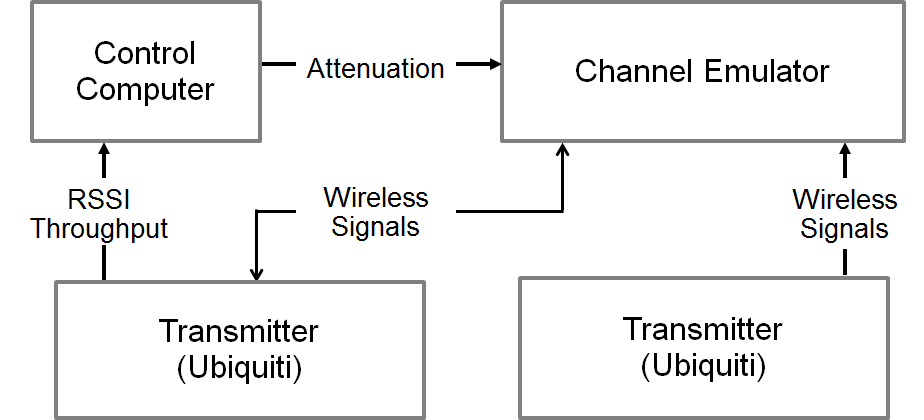
\includegraphics[width=85mm]{figures/emulator2}
%\vspace{-0.1in}
\caption{Experimental setup for channel emulator.}
\label{fig:in-door experiment}
\vspace{-0.1in}
\end{figure}

%\subsection{Signal Level Context-aware information}
\subsection{Experimental Design for In-field Data Collection}
\label{subsec:insitu}
We now describe the in-field experimental design to obtain a data set for
evaluating our multiband algorithms. Two Gateworks boards, each containing
the aforementioned four radios, are installed on two cars.  One node is always
the receiver and at a fixed location. The other node is always the 
transmitter and travels 
around the block of a public park as shown in Figure~\ref{fig:infield}.
One loop of the route will be used as a unit of training in the next section.

\begin{figure} [h]
%\vspace{-0.1in}
\centering
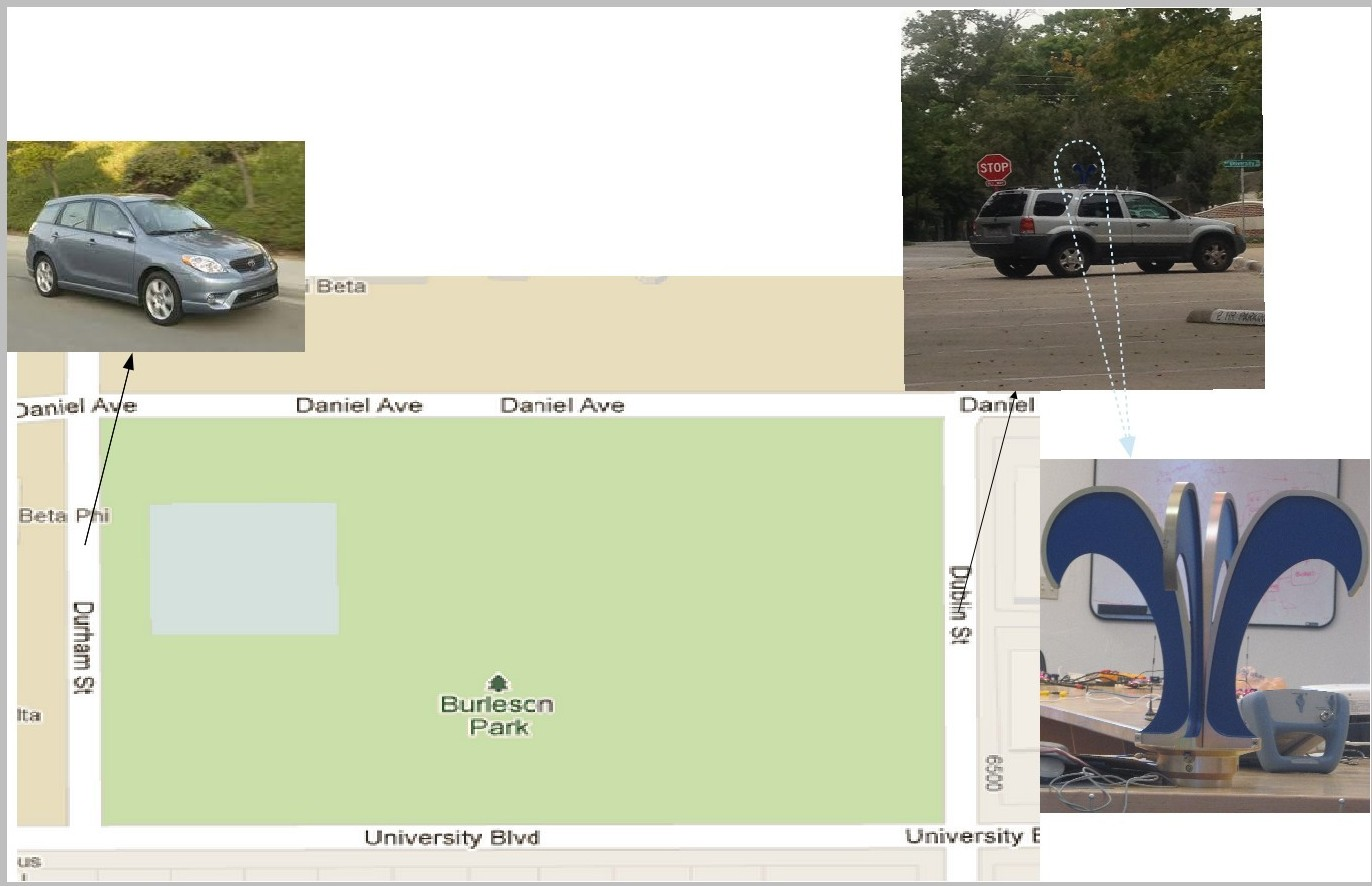
\includegraphics[width=85mm]{figures/infield}
\vspace{-0.1in}
\caption{In-field Experimental Setup.}
\label{fig:infield}
\vspace{-0.1in}
\end{figure}

During each loop, the transmitter sends a fully-backlogged UDP flow
using {\it iperf} on each of the four radios simultaneously.  To
focus on band selection and ensure the greatest range, we disable autorate and use a fixed data rate
of 6 Mbps. The receiver continually performs a {\it tcpdump} of all
received 802.11 packets~\cite{jacobson1989tcpdump}. Additionally, a
QH 400 Quad Ridge Horn Antenna (shown in Figure~\ref{fig:infield}) is 
connected to a Rhode \& Schwarz FSH8 mobile spectrum analyzer at the 
receiver to monitor spectral activity. Then, based on the 
time stamps, we remove 802.11 packets from the spectral trace 
so that only non-802.11 interference will contribute to $P_N^i$.

\begin{figure} 
%\vspace{-0.1in}
\centering
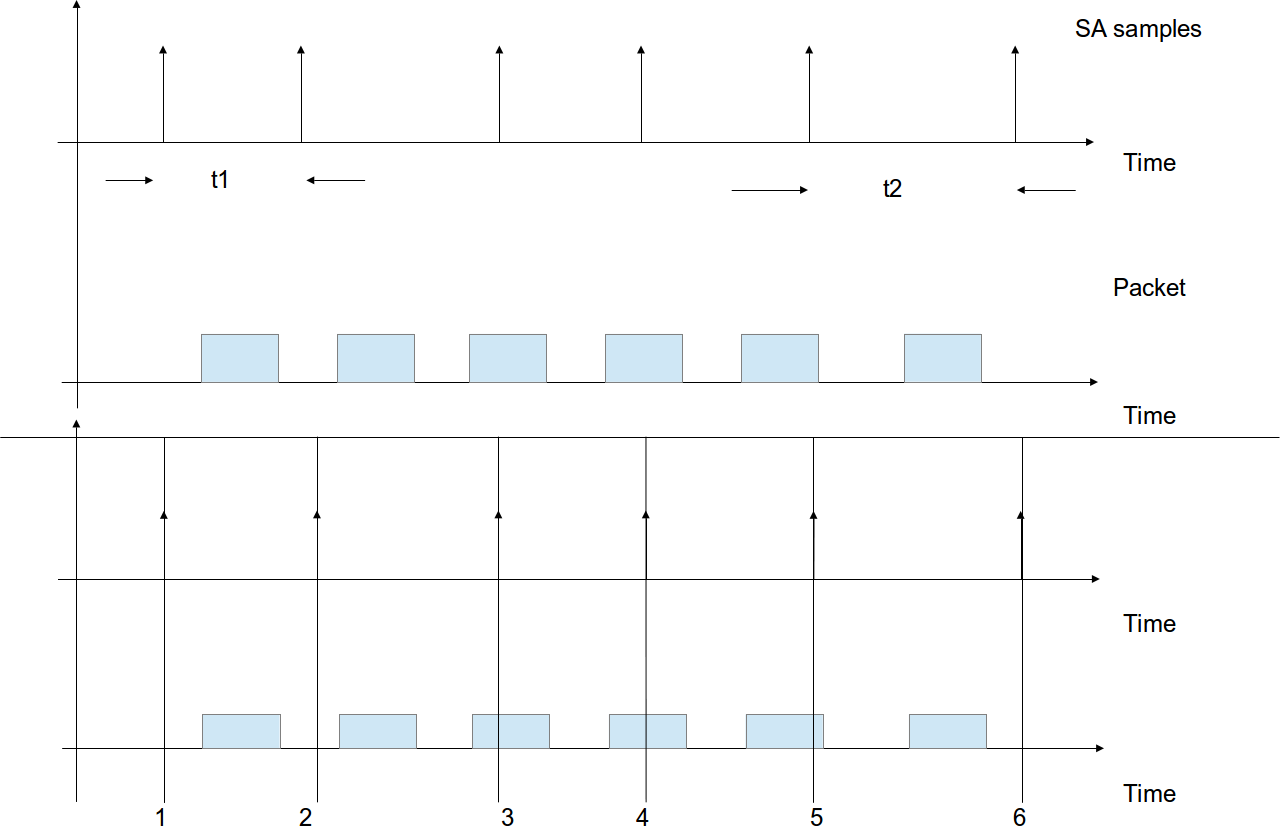
\includegraphics[width=85mm]{figures/sa_process}
\vspace{-0.1in}
\caption{Spectrum Analyzer Data Processing.}
\label{fig:sa_process}
\vspace{0.1in}
\end{figure}

Figure~\ref{fig:sa_process} shows how we obtain the
non-802.11 interference, $P_N^i$. We expunge the spectrum analyzer
(SA) samples which overlap in time with the dumped 802.11 packets,
such as packets 3, 4, and 5. Then, the reported interference value
will not contain the received power from 802.11 packets, which have
already been considered via the activity level, $A$.

The in-field data is processed offline where data from all instruments
involved is synchronized based on the GPS time stamps. 
As discussed in Section~\ref{subsec:ichannel}, the throughput of each radio
is normalized based upon emulator experiments to account for any
manufacturing differences.


\section{Performance Analysis of Algorithms}
\label{sec:vncdata process}

We now evaluate our proposed
algorithms with the experimental setup described in
Sections~\ref{subsec:ichannel} and \ref{subsec:insitu}.
The metrics of
{\it Accuracy} and {\it Throughput Gap} are used in the evaluation.
We consider each second of the in-field trace and
observe the frequency band that had the highest 
throughput.  The \emph{Accuracy} is defined as the percentage of 
best band predictions that match the observed optimal band, where a prediction
is made each second.  Conversely, the \emph{Throughput Gap} is defined
as the difference between the throughput observed on the optimal band
and the throughput achieved by the predicted best band over the
throughput of the observed optimal band. 
In the situation where the optimal band is not chosen, the throughput could be close between the chosen and optimal bands, meaning that the
incorrect band choice did not result in a large throughput loss. Thus, the 
\emph{Throughput Gap} metric captures the severity of the incorrect choice.

%\begin{align}
%\label{equation:df accuracy}
%Accuracy = \frac{Correct\ Prediction\ Slots}{All\ Predict\ Time\ Slots}
%\end{align}
%
%\emph{Throughput Gap} is the deference between the performance of estimation throughput and measured best throughput as defined in Formula \ref{equation:df gap}.
%
%\begin{align}
%\label{equation:df gap}
%Throughput\ Gap = \frac{\sum{Max\ Tpt- Estimate\ Band\ Tpt}}{\sum{Max\ Tpt}}
%\end{align}

Since the \emph{SNR-based Throughput Look-up Algorithm} requires only 
emulator-based training, the \emph{Accuracy} and \emph{Throughput Gap} can 
be calculated for all loops of the in-field trace.  However, the 
\emph{Location-based Look-up Algorithm} and \emph{Region-based Decision
Tree Algorithm} require in-field training. Thus, the data set must be
divided into a training set and testing set for evaluation.

\begin{figure}
%\vspace{-0.0in}
\centering
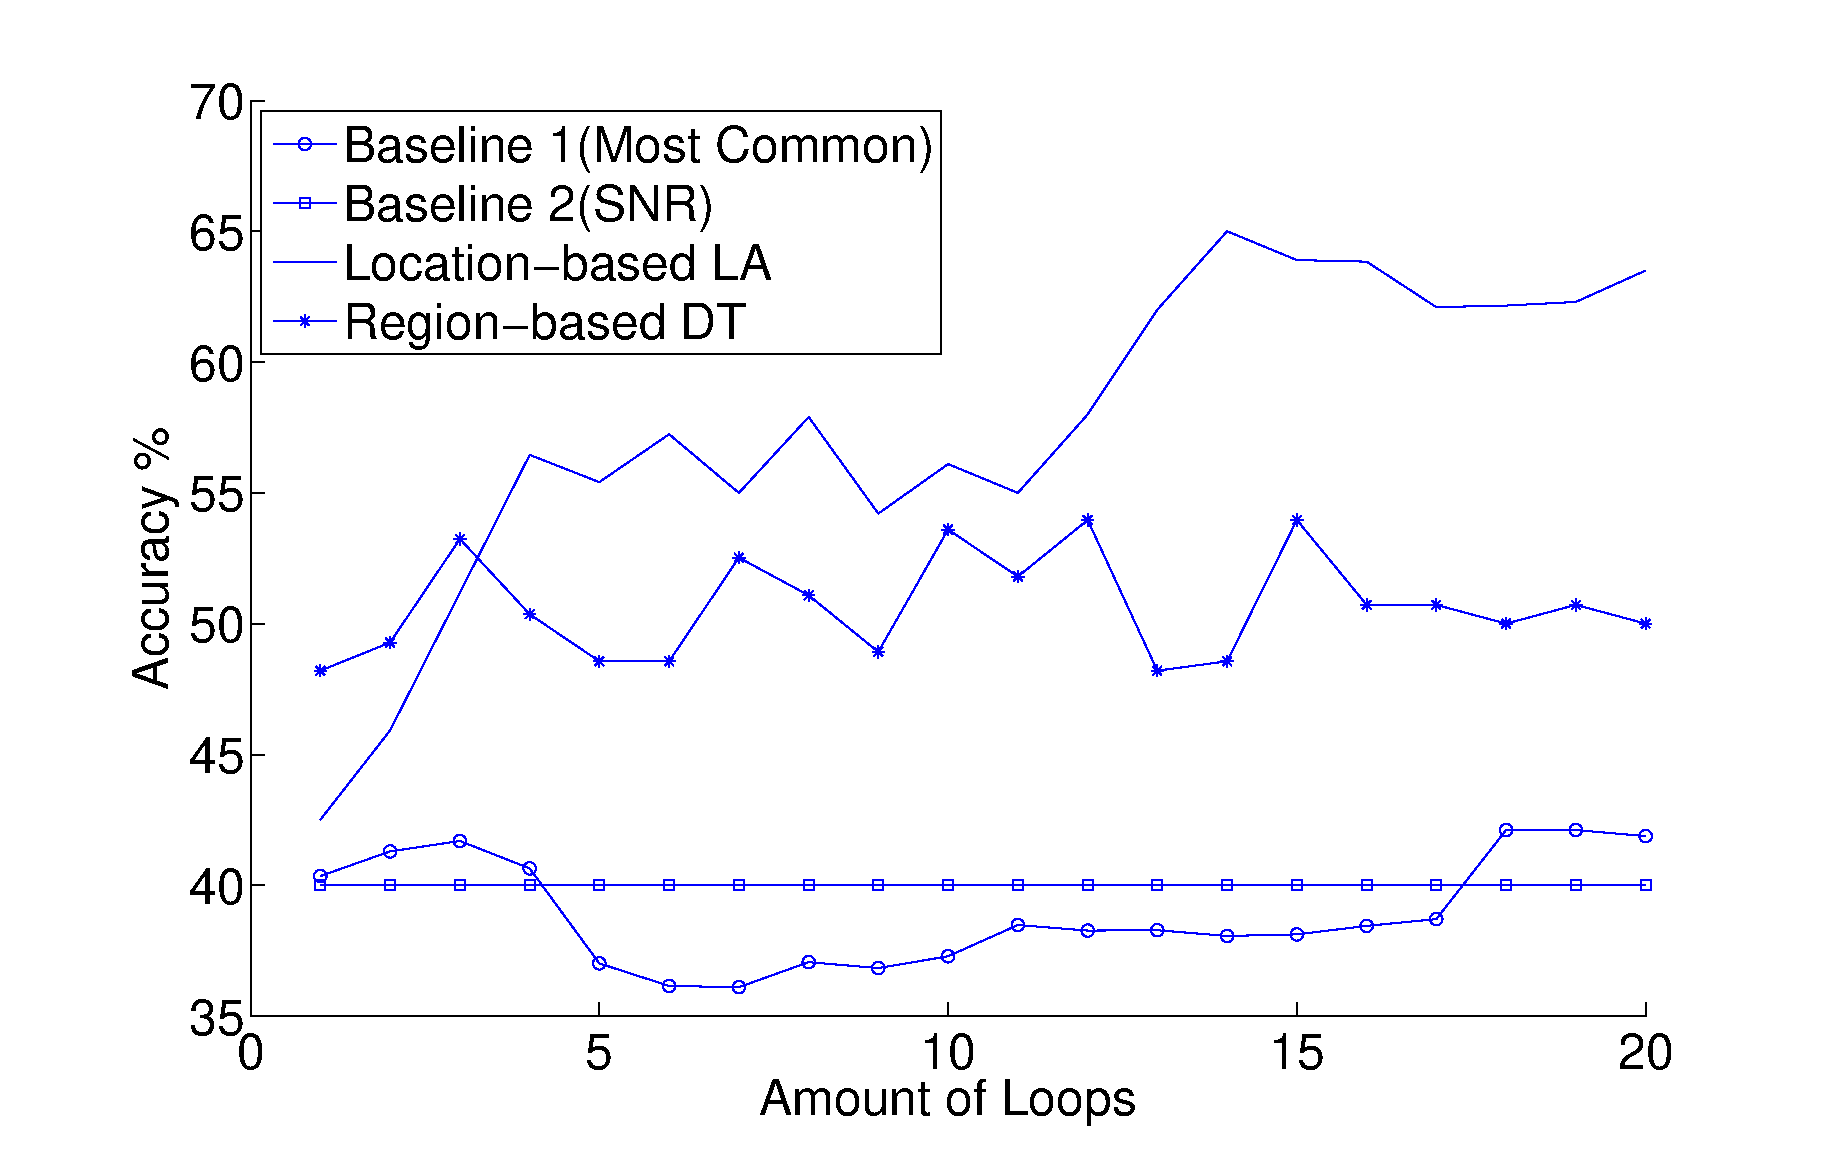
\includegraphics[width=68mm]{figures/performance_accuracy}
\vspace{-0.1in}
\caption{Accuracy of the four multiband algorithms.}
\label{fig:performance}
%\vspace{-0.0in}
\end{figure}

In Figure \ref{fig:performance}, we show the aforementioned \emph{Accuracy}
of the four multiband algorithms in selecting the band with the highest
throughput. The x-axis represents the number of loops around the
block of the mobile transmitter (shown in 
Figure~\ref{fig:infield}) that will be used by the machine-learning-based
algorithms. We use the same training and testing set to compare 
the \emph{Location-based Look-up Algorithm} and \emph{Region-based
Decision Tree Algorithm}. From the results, we observe the following:

\begin{itemize}
\item
At each loop, the first baseline algorithm, \emph{Most Commonly-Selected
Band}, uses the band with the greatest long-term average of the percentage
of time that band yields the highest throughput over the previous loops.
The accuracy ranges from 36.1\% to 42.9\%.
\item
The second baseline algorithm, \emph{SNR-based Throughput Look-up},
maintains 39.2\% across all the loops since it relies only on 
emulator-based training.
\item 
The \emph{Region-based Decision Tree Algorithm} has an accuracy ranging
from 48.2\% to 54.0\% but contains many dips due to the relationship
between the context information and the distribution of the best band
choice changing on a loop-by-loop basis. Additional training data 
slightly improves the decision structure overall but primarily induces
additional noise in the training process.
\item 
The \emph{Location-based Look-up Algorithm} begins with an accuracy of
42.5\% but improves the most out of any algorithm to finish with an 
accuracy 62.5\% with the highest accuracy of 65.0\% occurring after loop 14.
Additional in-field training loops are likely to further improve the multiband
selection accuracy.
\end{itemize}

\begin{figure}
\vspace{-0.1in}
\centering
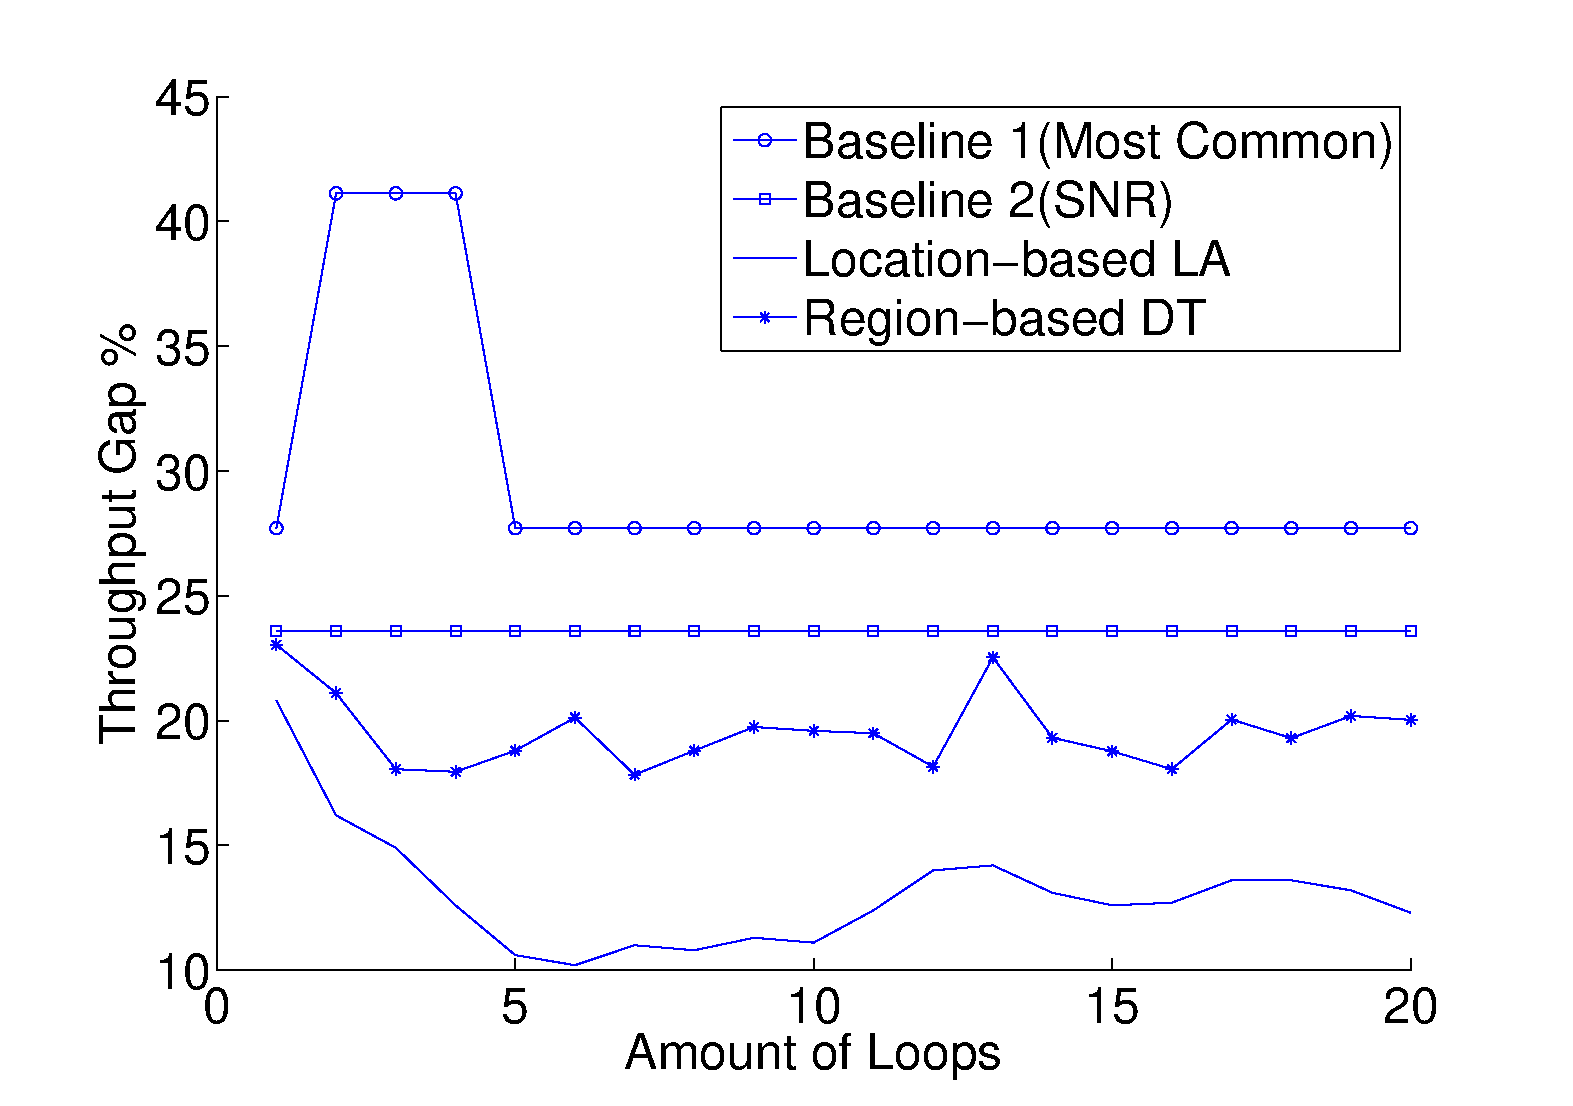
\includegraphics[width=65mm]{figures/performance_gap}
\vspace{-0.1in}
\caption{Throughput Gap of the four multiband algorithms.}
\label{fig:performance_gap}
\vspace{0.1in}
\end{figure}

Figure~\ref{fig:performance_gap}, 
depicts the \emph{Throughput Gap} of the four algorithms we evaluated and shows the following.

\begin{itemize}
\item
The \emph{Most Commonly-Selected Band Algorithm} has two different modes
of throughput gap based upon which band has the highest long-term 
percentage.  For loops 2-4, the choice is 5.8 GHz, which has a gap of 
41.1\% using the test set. For all other loops, the choice is 2.4 GHz, 
which has a gap of 27.7\%. 
\item 
The \emph{SNR-based Throughput Look-up Algorithm} shows a baseline  
performance of 23.6\% for the throughput gap.
\item 
The \emph{Region-based Decision Tree Algorithm} benefits from
additional training, going from a throughput gap of 23.0\% to 20.0\%.
Spatial and temporal changes to context information bring dips
to the curve as discussed earlier.
\item
Finally, the \emph{Location-based Look-up Algorithm} takes only 6 loops
of training to reach its lowest value of 10.2\% in terms of throughput
gap. From loops 1 to 20, the throughput gap goes from 20.8\% to 12.3\%,
which might still be improved upon with additional training.
\end{itemize}

\begin{figure}
%\vspace{-0.0in}
\centering
\includegraphics[width=75mm]{figures/region_map}
\vspace{-0.1in}
\caption{Spatially splitting experimental area into 8 regions.}
\label{fig:region map}
%\vspace{-0.0in}
\end{figure}

\begin{figure}
\vspace{-0.1in}
\centering
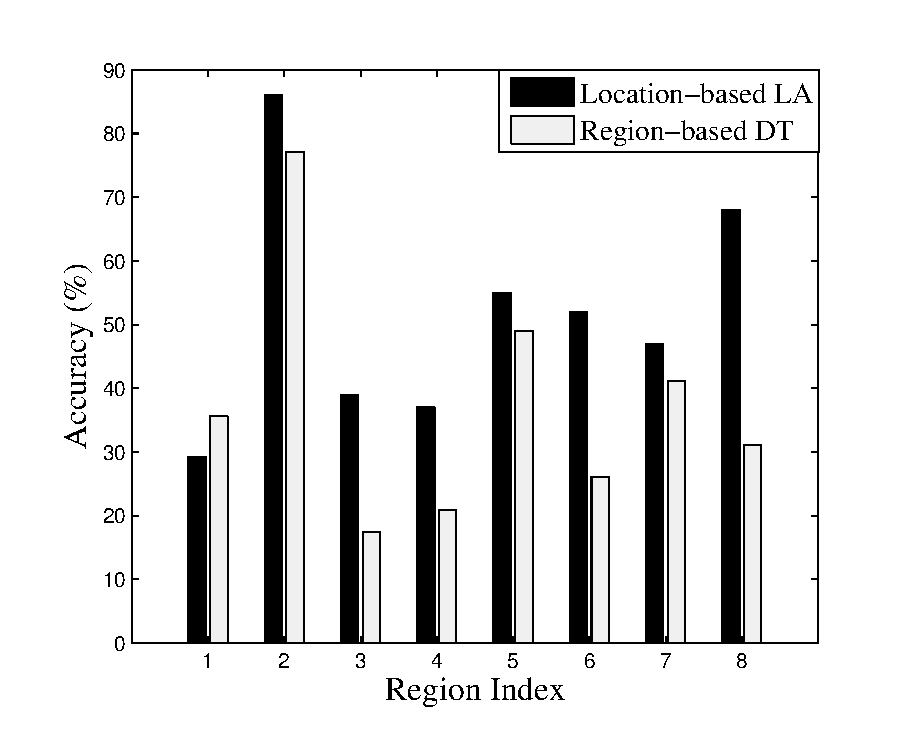
\includegraphics[width=65mm]{figures/mvsl}
\vspace{-0.1in}
\caption{Accuracy when dividing training set into 8 regions.}
\label{fig:mvsl}
\vspace{0.1in}
\end{figure}

We now consider the effect of further sub-dividing in-field experimental testing data into regions for our \emph{Location-based Look-up Algorithm} 
and \emph{Region-Based Decision Tree Algorithm}. To do so, we divide the    
loop around the park into eight regions as shown in Figure \ref{fig:region map},
which has two competing effects: (i.) Smaller regions allow similar experimental
data to be used in the training process, potentially improving the decision
structure. (ii.) For a given training set, dividing it into regions reduces
the number of training points for the machine learning algorithms, potentially
weakening the decision structure.  In Figure~\ref{fig:mvsl}, we observe 
the \emph{Accuracy} of the eight regions for both algorithms.
\begin{itemize}
\item
In all but Region 1, the \emph{Location-based Look-up Algorithm} has better 
performance than \emph{Region-based Decision Tree Algorithm}. The improved
accuracy of the former algorithm can be attributed to its ability to
distinguish each point's relative distance to the middle of the region
For the \emph{Region-based Decision Tree Algorithm}
to capture such a notion, the regions would have to be further sub-divided,
increasing the number of trees and reducing the training set per tree.
\item
For this training set, the reduction in training data caused by the
regional divisions had a net loss on the performance of the \emph{Region-based Decision Tree Algorithm}. However, if the training set was much larger
for a given area, the net effect of regional divisions could be positive.
\end{itemize}

%We have investigated the performance of the algorithms in one experimental data set and shown the gains of them. Multiband channels are complex system that knowing more information can make better decisions. 




%\section{Related Work}
\label{sec:related}

Cognitive Radio could be a powerful tool for the utility of the Spectrum Opportunity~\cite{haykin2005cognitive}.
Analog TV bands will be released for wireless communication brings opportunity to combine current wireless bands and new available bands for performance improvement employing Cognitive Radio methods~\cite{MOAR}. 


%Related research
A bunch of work has been done on radio-scene analysis and channel identification for utility of channel adaptation dating back to Simon Haykin~\cite{haykin2005cognitive}.
Some work of Multi-bands/Multi-channels in
cognitive radios focus on optimize performance, such as avoiding frequency diversity~\cite{rahul2009frequency}. 
In~\cite{OAR} an opportunistic algorithm is introduced to balance the cost of spectrum sensing, channel switching and the gain of these activities.


%Our work
Our work is motivated by prospective releasing band used for TV now and exploit the comparison across all the available bands in the future. 
It is an extension of multi-channel adaptation. 
Most of the published research focus on the stopping rules of spectrum sensing~\cite{sabharwal2007opportunistic, OAR}. In contrast, we use the data and framework to classify the performance across different bands based on the parameters we get from the context information.
%{\bf .} 


\section{Summary}
\label{sec:vncsummary}


In this chapter, we investigated multiband adaptation to leverage the propagation and context for vehicular applications. 
We did so by proposing two machine-learning-based schemes and compared their
performance against two baseline schemes.
In our experimental analysis, we evaluated the performance of these algorithms 
in the field on an off-the-shelf platform.
Experimental results demonstrate that the proposed algorithms can 
achieve up to 49.3\% greater throughput than the baseline algorithms
with an accuracy up to 65\%. In future work, we will study the impact that
multiple diverse environments have on the training as well as evaluate
the optimal use of multiple, diverse radios in unison.
%Since mobile networks have limited
%energy and training in multiple environment has not been investigated, in future work we plan to examine the influence of diverse environment and energy efficiency of
%the simultaneous use of multiple, diverse radios.



\chapter{Spectrum Adaptation for Single Hop Access Networks} 
\label{ch:winmee}



%
\section{Introduction}
\label{sec:introduction}


%Background
Drivers can benefit from a wide array of vehicular applications ranging from real-time traffic monitoring and
safety applications to {\it infotainment} applications spanning news, weather, audio, or video streams.  
However, the continuous use of such applications is limited due to the challenge of transmitting over 
highly-dynamic vehicular wireless channels. In such networks, the increasing availability of different 
frequency bands with correspondingly diverse propagation characteristics could allow flexibility and 
robustness of vehicular links. Even with such spectral flexibility, links are extremely tenuous, 
demanding nearly instantaneous decisions in order to remain connected and motivating an algorithm that
can find the appropriate frequency band quickly and according to the current application.

Prior work has considered a number of challenges in
leveraging the digital white space frequencies including spectrum sensing, frequency-agile operation,
geolocation, solving stringent spectral mask requirements, and providing reliable service
in unlicensed and dynamically changing spectrum along with corresponding 
protocols~\cite{shellhammer2009technical}. In particular, there has recently been an acceleration
in spectrum sensing work~\cite{rayanchu2011fluid, kim1996pulse,cabric2004implementation}. Based on 
these works, protocols have been built for multi-channel and/or multi-band wireless operation~\cite{MOAR,
raychaudhuri2003spectrum,sabharwal2007opportunistic}.  Other works have presented a method for searching the most efficient 
transmission channel~\cite{mo2005comparison}, discovering channel information from limited 
measurements~\cite{rayanchu2011fluid, sabharwal2007opportunistic}, and estimating 
channel quality through limit information~\cite{MOAR}. 

While these works have considered spectral activity and developing protocols and algorithms to 
find spectral holes, less of a focus has been on coupling such information with the propagation 
changes that frequency differences of hundreds of MHz to GHz could have on the band decision.  
Moreover, it is well known that propagation greatly depends on the environment in 
operation~\cite{rappaport}.  Thus, 
knowledge of the environment in operation could allow the relationship between received power 
differences across multiple frequency bands to have much greater accuracy.  In this paper, 
we present a multi-band adaptation protocol which leverage in-situ wireless propagation 
measurements and level of per-band activity with machine learning techniques that make a 
band choice according to application-specific performance metrics. To do so, we use an
off-the-shelf platform that allows direct experimentation across four different wireless
frequency bands simultaneously from 450 MHz to 5.8 GHz while maintaining the same physical
and media access layers.

%, it is hard to get a predict SNR just from the pathloss equation. To predict the SNR, a context-aware method is involved in this paper and combine with other methods to predict parameters for multiband adaptation.

%Activity level
%There are other factors will influence the wireless performance in different bands. One factor we are focusing on is the crowd level in different bands. Tons of wireless devices have been used all the world and completed with each other. 
%A concept \emph{activity level} which is the percentage of time the interference nodes occupied is included in this framework to qualify the crowd level. 
%In our framework we analyze the effect of crowd level using \emph{activity level} to estimate the available transmission time for a dominant factor. As a result, we formulate the \emph{Multi-band} adaptation problem to the throughput calculated from known Signal Strength and received packages. We verified the protocol on emulated, indoor and in field experiments to experimentally evaluate our approach. 

%Framwork
%The process of our framework is used to predict the performance involve context-aware information of multi bands. The context-aware information is from ideal channel(Emulator), indoor, in-field experiments. Support Vector Machine(SVM) is employed to connect the dynamic information to the context-aware information.  
%We evaluate our methods by indoor and in field experiments across 4 bands(700MHz, 900MHz, 2.4GHz, 5.8GHz), and show that in certain scenarios our approach can 
%predict the SNR more accuracy than pathloss equation and 
%Through the framework, the performance can be improved by fixme employing multi-band comparing to single wireless band.


%Problem formulation
%To get the two parameters for the performance estimation, both theoretical and context-aware methods are involved in this paper. Based on these parameters and other fixed factors according to specific environment, such as channel type, path-loss exponent and speed of wireless nodes, we are approaching to the basic problem of multi-band adaptation. 
%The basic problem of interest is as follows: \emph{Given the information of one band, get the information of other bands.}
%To solve the problem, 
%we first build a \emph{Ideal Channel Performance Context-Aware database} through the measured data from channel emulator across a wide range of different scenarios. 
%Then, based on the database and the parameters, a tunable threshold connect the \emph{Signal Strength} and the performance of different bands.

%Wireless channels are classed to different types based on the speed, propogation, noise ando so on. A simplistic characterization of channel type example could be a vehicular A in this paper. The basic problem of interest is as follows: \emph{given the channel type and Signal Strength, find the wireless band that achieves the highest throughput.}
%To solve the problem, we first build a \emph{Ideal Channel Look-Up Table} through the measured data from channel emulator across a wide range of different scenarios. Based on this , an ideal throughput for particular signal strength without noise and interference can be connected. The protocol also holds a tunable threshold parameter that determines when the \emph{Signal Strength} is different enough from others.



%Contributions  fixme
The main contributions of our work are as follows:
\begin{itemize}
\item We first formulate the problem of selecting the optimal 
frequency band according to diverse application performance metrics
to be used in the following multiband algorithms.
\item We consider three different algorithms for comparison.  First, we consider a scheme
in which the throughput is achieved on an emulated channel (historical information) for
the current received signal level. We then adjust the predicted best band choice according to the current activity
level (real-time information). 
Second, we consider an approach based on machine learning which
considers prior throughput for a given received signal and activity level
combination.  
Third, we include user location in addition to both the emulated channel and machine learning in addition to the received signal and activity level.
%Third, we consider a second machine learning approach which considers user
%location in addition to the received signal and activity level.
\item We perform V-2-\it{Base Station} experiments to evaluate each algorithm on a repeatable pattern that
%spans multiple environment types (campus, residential, and suburban) with various activity
spans in-field environment with various activity
levels and propagation characteristics within the regions. 
\end{itemize}


%\item We define an \emph{Activity Level} and enroll the concept to dynamic throughput prediction framework. The \emph{Activity Level} can describe the channel interference in time domain.
%\item We propose a simple framework that provides a way to compare the throughput across 4 different bands. Prediction the throughput across multi-band is the precondition to select a band for transmission.  
%\item We build the Look-up Table across different bands, channel models. The LUT refer to the ideal status of the channels across multi bands. It bring benifet for the work in the future.
%We experimentally analyze our framework with simulation and in-field experiments on off-the-shelf hardware platform. The platform is Gateworks 2358 board with 802.11-based radios in different frequency bands. All the radios have a physical layer based on the IEEE 802.11 a/g standard and other sensors for data collection.

The remainder of this paper is organized as follows. In Section II, we present the multiband adaptation problem and proposed algorithms. Section III discusses experimental evaluation of the multiband algorithms. We present related work in Section IV. A summary and discussion of future work is included in Section V.

%Chris: Should we remove the V_2_V experiments in the paper?

\input{multiband_winmee/problemformulation}
\section{Data Process}
\label{sec:experiment}

Fixme


%Detail may not useful
Parsing script
In our experiments, we are constantly collecting large amounts of data, including the received signal level, current location, velocity, and time of day. Working with the memory-limited Gateworks boards, it became necessary to implement a solution to collect large amounts of data without exhausting the available memory space on the boards. Thus, we compiled a script to parse an undetermined number of data files containing the raw data collected from the ongoing experiments. Utilizing the Perl programming language, which the Gateworks boards are capable of running, the script scans every file in a directory we specify and parses them, looking specifically for signal level, lat/long location, velocity, and time data recorded from the experiments. Upon finding this information, the script reformats the data by placing it into a .csv file. Additionally, using the location data, the script calculates the  distance between the transmitting and receiving boards and adds this information to the .csv file. Upon parsing the data, the raw experimental data files can simply be delete from memory, freeing up space for the data of subsequent experiments.

Activity monitor script
For in-situ experiments, the need became apparent to track the number of new incoming packets and compare it with the number of previously received packets. Additionally, this needed to be done for each of the four wireless radios on the board. In doing this, we identify the most efficient frequency band to transmit data. To implement this system, a script was needed to run efficiently in the background while experiments were taking place. To achieve this, we wrote a bash shell script to run directly on the board without relying on any higher level programming language that could potentially cause greater performance overhead. As a result, the script only consumes one to two percent of CPU resource. The script begins by examining the received bytes across each radio for a length of 30 seconds and placing the bytes received each second on a new line in a file. Upon the completion of the 30 second buffering time period, the next second of received bytes on each radio is read and compared with the last 30 seconds of received data. This ratio of the most recent received data to old received data is then calculated and written to four files, one for each radio, for its subsequent use in selecting which radio to transmit/receive from.


%\section{Related Work}
\label{sec:related}
%%fixme add the daparowrds
%The conventional definition of the spectrum opportunity, which is often defined as "A band of frequencies that are not being used by the primary user of that band at a particular time in a particular geographic area."\cite{kolodzy2001next}


Elecronmagnetic radio spectrum is a natural resource licensed by governments.  the Federal Communications Commission(FCC) published a report prepared by the Spectrum-Policy Task Force, discussed improving the way to manage this resource in the United States \cite{federal2002spectrum}. 

The limited resource make people find new ways to improve the effciency of the frquency resource utility. There are two methods to arrive this target. First is the underlay approach, constraints on the transmission power of second users. Second is the overlay approach, identify and exploit spatial and temporal spectrum white space by second users \cite{zhao2007survey}.
The first approaching require more support from the hardware, the second approaching can be achieved by soft-ware radios only. The frequency is not occupacied all the time in all the regions.


%ways to improve the frequency efficient



The underutilization of the electromagnetic spectrum leads to a definition of \emph{Spectrum Opportunity} as a band of frequencies assigned to a primary user, but at a particular time and specific geographic location, the band is not being utilized by that user \cite{kolodzy2001next}.



%Cognitive Radio

%fixme FCC definition
%The definition adopted by Federal Communications Commission(FCC):"Cognitive radio: A radio or system that senses its operational electromagnetic environment and can dynamically and autonomously adjust its radio operating parameters to modify system operation, such as maximize throughput, mitigate interference, facilitate interoperability, access secondary markets."
The concept of \emph{Cognitive Radio} is introduced as a novel approach for improving the utilization of the wireless spectrum and the tasks for cognitive radio is summarized in \cite{haykin2005cognitive}. The three on-line cognitive tasks include: \emph{Radio-scene analysis, Channel identification, Transmit-power control and synamic spectrum management} \cite{haykin2005cognitive}.
Underutilized terrestrial TV bands will be able to be used by wireless communication. Combine different bands to create Multi-bands/Multi-channels system is a new field of \emph{Cognitive Radio} to improve the performance of wireless systems in different
environments(e.g., as in ~\cite{MOAR}). 

%Multi-channel
A bunch of work has been done on \emph{Radio-scene analysis} and \emph{Channel identification} dating back to Simon Haykin \cite{haykin2005cognitive}.
Some work of Multi-bands/Multi-channels in
cognitive radios focus on optimize performance, such as avoiding frequency diversity \cite{rahul2009frequency}. 
In \cite{OAR} an opportunistic algorithm is intorduced to balance the cost of \emph{spectrum sensing, Channel switching} and the gain of these activities.
%fixme, add more multichannel and add pathloss exponent

%spectrum sensing

One of the most important components of the congnitive radio concept is the ability to measure, sense, learn and be aware of the parameters related to the radio channel characteristics, availability of spectrum and power, radios operating envrionment \cite{yucek2009survey}. Spectrum sensing becomes the most important component for the estabilishment of congnitive radio. \cite{yucek2009survey}. 





%Adaptation algorithms
There is a lot of recent research on the design of adaptation algorithms, both rate adaptation and \emph{band/channel} adptation of cognitive radio systems. These researches are focusing on the \emph{Spectrum sensing and Channel switching strategies}.

\textbf{Evaluation of Channel Conditions}. Channel condition is the most important component of adaptation. 
There are two classes of rate adaptation mechanisms that have been developed. 
These mechanisms are focused on rate adaptation. The first generation adaptation algorithms are loss-triggered. The adaptation algorithm based on the statistics of a previous period of transmission. 
Second generation rate adaptation schemes diagnose the cause of a loss and appropriately adjust the data rate \cite{biaz2008rate, camp2010modulation}, such as a SNR-triggered protocol. 
Our work consider both the statistics information of the previous transmission and the dynamic information in context-aware based channel qualification.

\textbf{Evaluation of Adaptation}. Most of the prior work of rate adaptation protocols has investigated the effectiveness via throughput comparison \cite{camp2010modulation}. This is the metric we also employ in the paper to evaluate the performance. Furthermore, we also evaluate the amount of context-aware information in prediction.
 
\textbf{Primary Second User}. Some other works focus on Multi-channel which bandwidth range limits in 2.4GHz \cite{MOAR} or in a continuous bandwidth considering frequency diversity \cite{rahul2009frequency}. 
Significant research on the design of channel selection algorithms has been done \cite{radunovic2011dynamic,raniwala2005architecture}. Algorithms are generated for second user to distinguish whether the channel is free or in less utility state as soon as possible \cite{cordeiro2007c}. These works indicate the way to employ limit frequency work in high efficiency. In contrast, we are trying to improve the wireless performance taking more frequency bands.

Our work is motivated by prospective white band using for TV today and exploit the comparison across all the avaiable bands in the future. It is a kind of extention of multi-channel adaptation. Our approach classifies the performance based upon combination of in-field measurents and ideal channel conditions on \emph{channel emulator}. Most of the research focus on the stopping rules of spectrum sensing \cite{sabharwal2007opportunistic, OAR}. In contrast, we use the data and framework to classify the performance across different bands based on the parameters we get from the context-aware information.
{\bf .} 


%\chapter{Multiband Hetegeneous Access Point Optimization} 
%\label{ch:moa}
\input{multiband_moa/problemformulation}
\section{Data Process}
\label{sec:experiment}

Fixme


%Detail may not useful
Parsing script
In our experiments, we are constantly collecting large amounts of data, including the received signal level, current location, velocity, and time of day. Working with the memory-limited Gateworks boards, it became necessary to implement a solution to collect large amounts of data without exhausting the available memory space on the boards. Thus, we compiled a script to parse an undetermined number of data files containing the raw data collected from the ongoing experiments. Utilizing the Perl programming language, which the Gateworks boards are capable of running, the script scans every file in a directory we specify and parses them, looking specifically for signal level, lat/long location, velocity, and time data recorded from the experiments. Upon finding this information, the script reformats the data by placing it into a .csv file. Additionally, using the location data, the script calculates the  distance between the transmitting and receiving boards and adds this information to the .csv file. Upon parsing the data, the raw experimental data files can simply be delete from memory, freeing up space for the data of subsequent experiments.

Activity monitor script
For in-situ experiments, the need became apparent to track the number of new incoming packets and compare it with the number of previously received packets. Additionally, this needed to be done for each of the four wireless radios on the board. In doing this, we identify the most efficient frequency band to transmit data. To implement this system, a script was needed to run efficiently in the background while experiments were taking place. To achieve this, we wrote a bash shell script to run directly on the board without relying on any higher level programming language that could potentially cause greater performance overhead. As a result, the script only consumes one to two percent of CPU resource. The script begins by examining the received bytes across each radio for a length of 30 seconds and placing the bytes received each second on a new line in a file. Upon the completion of the 30 second buffering time period, the next second of received bytes on each radio is read and compared with the last 30 seconds of received data. This ratio of the most recent received data to old received data is then calculated and written to four files, one for each radio, for its subsequent use in selecting which radio to transmit/receive from.




\Section{Spectrum Adaptation for Scant White Space Resource} 
\label{ch:whitecell}



%
\section{Introduction}
\label{sec:introduction}


%Background
Drivers can benefit from a wide array of vehicular applications ranging from real-time traffic monitoring and
safety applications to {\it infotainment} applications spanning news, weather, audio, or video streams.  
However, the continuous use of such applications is limited due to the challenge of transmitting over 
highly-dynamic vehicular wireless channels. In such networks, the increasing availability of different 
frequency bands with correspondingly diverse propagation characteristics could allow flexibility and 
robustness of vehicular links. Even with such spectral flexibility, links are extremely tenuous, 
demanding nearly instantaneous decisions in order to remain connected and motivating an algorithm that
can find the appropriate frequency band quickly and according to the current application.

Prior work has considered a number of challenges in
leveraging the digital white space frequencies including spectrum sensing, frequency-agile operation,
geolocation, solving stringent spectral mask requirements, and providing reliable service
in unlicensed and dynamically changing spectrum along with corresponding 
protocols~\cite{shellhammer2009technical}. In particular, there has recently been an acceleration
in spectrum sensing work~\cite{rayanchu2011fluid, kim1996pulse,cabric2004implementation}. Based on 
these works, protocols have been built for multi-channel and/or multi-band wireless operation~\cite{MOAR,
raychaudhuri2003spectrum,sabharwal2007opportunistic}.  Other works have presented a method for searching the most efficient 
transmission channel~\cite{mo2005comparison}, discovering channel information from limited 
measurements~\cite{rayanchu2011fluid, sabharwal2007opportunistic}, and estimating 
channel quality through limit information~\cite{MOAR}. 

While these works have considered spectral activity and developing protocols and algorithms to 
find spectral holes, less of a focus has been on coupling such information with the propagation 
changes that frequency differences of hundreds of MHz to GHz could have on the band decision.  
Moreover, it is well known that propagation greatly depends on the environment in 
operation~\cite{rappaport}.  Thus, 
knowledge of the environment in operation could allow the relationship between received power 
differences across multiple frequency bands to have much greater accuracy.  In this paper, 
we present a multi-band adaptation protocol which leverage in-situ wireless propagation 
measurements and level of per-band activity with machine learning techniques that make a 
band choice according to application-specific performance metrics. To do so, we use an
off-the-shelf platform that allows direct experimentation across four different wireless
frequency bands simultaneously from 450 MHz to 5.8 GHz while maintaining the same physical
and media access layers.

%, it is hard to get a predict SNR just from the pathloss equation. To predict the SNR, a context-aware method is involved in this paper and combine with other methods to predict parameters for multiband adaptation.

%Activity level
%There are other factors will influence the wireless performance in different bands. One factor we are focusing on is the crowd level in different bands. Tons of wireless devices have been used all the world and completed with each other. 
%A concept \emph{activity level} which is the percentage of time the interference nodes occupied is included in this framework to qualify the crowd level. 
%In our framework we analyze the effect of crowd level using \emph{activity level} to estimate the available transmission time for a dominant factor. As a result, we formulate the \emph{Multi-band} adaptation problem to the throughput calculated from known Signal Strength and received packages. We verified the protocol on emulated, indoor and in field experiments to experimentally evaluate our approach. 

%Framwork
%The process of our framework is used to predict the performance involve context-aware information of multi bands. The context-aware information is from ideal channel(Emulator), indoor, in-field experiments. Support Vector Machine(SVM) is employed to connect the dynamic information to the context-aware information.  
%We evaluate our methods by indoor and in field experiments across 4 bands(700MHz, 900MHz, 2.4GHz, 5.8GHz), and show that in certain scenarios our approach can 
%predict the SNR more accuracy than pathloss equation and 
%Through the framework, the performance can be improved by fixme employing multi-band comparing to single wireless band.


%Problem formulation
%To get the two parameters for the performance estimation, both theoretical and context-aware methods are involved in this paper. Based on these parameters and other fixed factors according to specific environment, such as channel type, path-loss exponent and speed of wireless nodes, we are approaching to the basic problem of multi-band adaptation. 
%The basic problem of interest is as follows: \emph{Given the information of one band, get the information of other bands.}
%To solve the problem, 
%we first build a \emph{Ideal Channel Performance Context-Aware database} through the measured data from channel emulator across a wide range of different scenarios. 
%Then, based on the database and the parameters, a tunable threshold connect the \emph{Signal Strength} and the performance of different bands.

%Wireless channels are classed to different types based on the speed, propogation, noise ando so on. A simplistic characterization of channel type example could be a vehicular A in this paper. The basic problem of interest is as follows: \emph{given the channel type and Signal Strength, find the wireless band that achieves the highest throughput.}
%To solve the problem, we first build a \emph{Ideal Channel Look-Up Table} through the measured data from channel emulator across a wide range of different scenarios. Based on this , an ideal throughput for particular signal strength without noise and interference can be connected. The protocol also holds a tunable threshold parameter that determines when the \emph{Signal Strength} is different enough from others.



%Contributions  fixme
The main contributions of our work are as follows:
\begin{itemize}
\item We first formulate the problem of selecting the optimal 
frequency band according to diverse application performance metrics
to be used in the following multiband algorithms.
\item We consider three different algorithms for comparison.  First, we consider a scheme
in which the throughput is achieved on an emulated channel (historical information) for
the current received signal level. We then adjust the predicted best band choice according to the current activity
level (real-time information). 
Second, we consider an approach based on machine learning which
considers prior throughput for a given received signal and activity level
combination.  
Third, we include user location in addition to both the emulated channel and machine learning in addition to the received signal and activity level.
%Third, we consider a second machine learning approach which considers user
%location in addition to the received signal and activity level.
\item We perform V-2-\it{Base Station} experiments to evaluate each algorithm on a repeatable pattern that
%spans multiple environment types (campus, residential, and suburban) with various activity
spans in-field environment with various activity
levels and propagation characteristics within the regions. 
\end{itemize}


%\item We define an \emph{Activity Level} and enroll the concept to dynamic throughput prediction framework. The \emph{Activity Level} can describe the channel interference in time domain.
%\item We propose a simple framework that provides a way to compare the throughput across 4 different bands. Prediction the throughput across multi-band is the precondition to select a band for transmission.  
%\item We build the Look-up Table across different bands, channel models. The LUT refer to the ideal status of the channels across multi bands. It bring benifet for the work in the future.
%We experimentally analyze our framework with simulation and in-field experiments on off-the-shelf hardware platform. The platform is Gateworks 2358 board with 802.11-based radios in different frequency bands. All the radios have a physical layer based on the IEEE 802.11 a/g standard and other sensors for data collection.

The remainder of this paper is organized as follows. In Section II, we present the multiband adaptation problem and proposed algorithms. Section III discusses experimental evaluation of the multiband algorithms. We present related work in Section IV. A summary and discussion of future work is included in Section V.

%Chris: Should we remove the V_2_V experiments in the paper?

\input{multiband_whitecell/problemformulation}
\input{multiband_whitecell/problemstatement}
\section{Data Process}
\label{sec:experiment}

Fixme


%Detail may not useful
Parsing script
In our experiments, we are constantly collecting large amounts of data, including the received signal level, current location, velocity, and time of day. Working with the memory-limited Gateworks boards, it became necessary to implement a solution to collect large amounts of data without exhausting the available memory space on the boards. Thus, we compiled a script to parse an undetermined number of data files containing the raw data collected from the ongoing experiments. Utilizing the Perl programming language, which the Gateworks boards are capable of running, the script scans every file in a directory we specify and parses them, looking specifically for signal level, lat/long location, velocity, and time data recorded from the experiments. Upon finding this information, the script reformats the data by placing it into a .csv file. Additionally, using the location data, the script calculates the  distance between the transmitting and receiving boards and adds this information to the .csv file. Upon parsing the data, the raw experimental data files can simply be delete from memory, freeing up space for the data of subsequent experiments.

Activity monitor script
For in-situ experiments, the need became apparent to track the number of new incoming packets and compare it with the number of previously received packets. Additionally, this needed to be done for each of the four wireless radios on the board. In doing this, we identify the most efficient frequency band to transmit data. To implement this system, a script was needed to run efficiently in the background while experiments were taking place. To achieve this, we wrote a bash shell script to run directly on the board without relying on any higher level programming language that could potentially cause greater performance overhead. As a result, the script only consumes one to two percent of CPU resource. The script begins by examining the received bytes across each radio for a length of 30 seconds and placing the bytes received each second on a new line in a file. Upon the completion of the 30 second buffering time period, the next second of received bytes on each radio is read and compared with the last 30 seconds of received data. This ratio of the most recent received data to old received data is then calculated and written to four files, one for each radio, for its subsequent use in selecting which radio to transmit/receive from.


\section{Conclusion}
\label{sec:conclusion}
In this paper, we investigated the multi-band adaption to leverage the propagation and context for vehicular utility. 
We did so by first testing and comparing the performance of different approaching multi-band selection algorithms. 
In our experimental analysis, we evaluated the performance of these algorithms on Gateworks hardware platform over in-field channels. 
Experimental results demonstrate that these algorithms can fit different utility environments. The accuracy of these algorithms can be up to 60.5\%.
Since for mobile utility, energy is limited, in the future work we plan to consider the energy efficient in multi-band adaptation.



\section{Conclusion}
\label{sec:conclusion}
In this paper, we investigated the multi-band adaption to leverage the propagation and context for vehicular utility. 
We did so by first testing and comparing the performance of different approaching multi-band selection algorithms. 
In our experimental analysis, we evaluated the performance of these algorithms on Gateworks hardware platform over in-field channels. 
Experimental results demonstrate that these algorithms can fit different utility environments. The accuracy of these algorithms can be up to 60.5\%.
Since for mobile utility, energy is limited, in the future work we plan to consider the energy efficient in multi-band adaptation.


\chapter{Spectrum Adaptation for Multihop Access Networks} 
\label{ch:wm}


\input{multiband_wm/problemformulation}
\input{multiband_wm/linearopt}
\input{multiband_wm/wmalgorithms}
\section{Data Process}
\label{sec:experiment}

Fixme


%Detail may not useful
Parsing script
In our experiments, we are constantly collecting large amounts of data, including the received signal level, current location, velocity, and time of day. Working with the memory-limited Gateworks boards, it became necessary to implement a solution to collect large amounts of data without exhausting the available memory space on the boards. Thus, we compiled a script to parse an undetermined number of data files containing the raw data collected from the ongoing experiments. Utilizing the Perl programming language, which the Gateworks boards are capable of running, the script scans every file in a directory we specify and parses them, looking specifically for signal level, lat/long location, velocity, and time data recorded from the experiments. Upon finding this information, the script reformats the data by placing it into a .csv file. Additionally, using the location data, the script calculates the  distance between the transmitting and receiving boards and adds this information to the .csv file. Upon parsing the data, the raw experimental data files can simply be delete from memory, freeing up space for the data of subsequent experiments.

Activity monitor script
For in-situ experiments, the need became apparent to track the number of new incoming packets and compare it with the number of previously received packets. Additionally, this needed to be done for each of the four wireless radios on the board. In doing this, we identify the most efficient frequency band to transmit data. To implement this system, a script was needed to run efficiently in the background while experiments were taking place. To achieve this, we wrote a bash shell script to run directly on the board without relying on any higher level programming language that could potentially cause greater performance overhead. As a result, the script only consumes one to two percent of CPU resource. The script begins by examining the received bytes across each radio for a length of 30 seconds and placing the bytes received each second on a new line in a file. Upon the completion of the 30 second buffering time period, the next second of received bytes on each radio is read and compared with the last 30 seconds of received data. This ratio of the most recent received data to old received data is then calculated and written to four files, one for each radio, for its subsequent use in selecting which radio to transmit/receive from.


%\section{Related Work}
\label{sec:related}
%%fixme add the daparowrds
%The conventional definition of the spectrum opportunity, which is often defined as "A band of frequencies that are not being used by the primary user of that band at a particular time in a particular geographic area."\cite{kolodzy2001next}


Elecronmagnetic radio spectrum is a natural resource licensed by governments.  the Federal Communications Commission(FCC) published a report prepared by the Spectrum-Policy Task Force, discussed improving the way to manage this resource in the United States \cite{federal2002spectrum}. 

The limited resource make people find new ways to improve the effciency of the frquency resource utility. There are two methods to arrive this target. First is the underlay approach, constraints on the transmission power of second users. Second is the overlay approach, identify and exploit spatial and temporal spectrum white space by second users \cite{zhao2007survey}.
The first approaching require more support from the hardware, the second approaching can be achieved by soft-ware radios only. The frequency is not occupacied all the time in all the regions.


%ways to improve the frequency efficient



The underutilization of the electromagnetic spectrum leads to a definition of \emph{Spectrum Opportunity} as a band of frequencies assigned to a primary user, but at a particular time and specific geographic location, the band is not being utilized by that user \cite{kolodzy2001next}.



%Cognitive Radio

%fixme FCC definition
%The definition adopted by Federal Communications Commission(FCC):"Cognitive radio: A radio or system that senses its operational electromagnetic environment and can dynamically and autonomously adjust its radio operating parameters to modify system operation, such as maximize throughput, mitigate interference, facilitate interoperability, access secondary markets."
The concept of \emph{Cognitive Radio} is introduced as a novel approach for improving the utilization of the wireless spectrum and the tasks for cognitive radio is summarized in \cite{haykin2005cognitive}. The three on-line cognitive tasks include: \emph{Radio-scene analysis, Channel identification, Transmit-power control and synamic spectrum management} \cite{haykin2005cognitive}.
Underutilized terrestrial TV bands will be able to be used by wireless communication. Combine different bands to create Multi-bands/Multi-channels system is a new field of \emph{Cognitive Radio} to improve the performance of wireless systems in different
environments(e.g., as in ~\cite{MOAR}). 

%Multi-channel
A bunch of work has been done on \emph{Radio-scene analysis} and \emph{Channel identification} dating back to Simon Haykin \cite{haykin2005cognitive}.
Some work of Multi-bands/Multi-channels in
cognitive radios focus on optimize performance, such as avoiding frequency diversity \cite{rahul2009frequency}. 
In \cite{OAR} an opportunistic algorithm is intorduced to balance the cost of \emph{spectrum sensing, Channel switching} and the gain of these activities.
%fixme, add more multichannel and add pathloss exponent

%spectrum sensing

One of the most important components of the congnitive radio concept is the ability to measure, sense, learn and be aware of the parameters related to the radio channel characteristics, availability of spectrum and power, radios operating envrionment \cite{yucek2009survey}. Spectrum sensing becomes the most important component for the estabilishment of congnitive radio. \cite{yucek2009survey}. 





%Adaptation algorithms
There is a lot of recent research on the design of adaptation algorithms, both rate adaptation and \emph{band/channel} adptation of cognitive radio systems. These researches are focusing on the \emph{Spectrum sensing and Channel switching strategies}.

\textbf{Evaluation of Channel Conditions}. Channel condition is the most important component of adaptation. 
There are two classes of rate adaptation mechanisms that have been developed. 
These mechanisms are focused on rate adaptation. The first generation adaptation algorithms are loss-triggered. The adaptation algorithm based on the statistics of a previous period of transmission. 
Second generation rate adaptation schemes diagnose the cause of a loss and appropriately adjust the data rate \cite{biaz2008rate, camp2010modulation}, such as a SNR-triggered protocol. 
Our work consider both the statistics information of the previous transmission and the dynamic information in context-aware based channel qualification.

\textbf{Evaluation of Adaptation}. Most of the prior work of rate adaptation protocols has investigated the effectiveness via throughput comparison \cite{camp2010modulation}. This is the metric we also employ in the paper to evaluate the performance. Furthermore, we also evaluate the amount of context-aware information in prediction.
 
\textbf{Primary Second User}. Some other works focus on Multi-channel which bandwidth range limits in 2.4GHz \cite{MOAR} or in a continuous bandwidth considering frequency diversity \cite{rahul2009frequency}. 
Significant research on the design of channel selection algorithms has been done \cite{radunovic2011dynamic,raniwala2005architecture}. Algorithms are generated for second user to distinguish whether the channel is free or in less utility state as soon as possible \cite{cordeiro2007c}. These works indicate the way to employ limit frequency work in high efficiency. In contrast, we are trying to improve the wireless performance taking more frequency bands.

Our work is motivated by prospective white band using for TV today and exploit the comparison across all the avaiable bands in the future. It is a kind of extention of multi-channel adaptation. Our approach classifies the performance based upon combination of in-field measurents and ideal channel conditions on \emph{channel emulator}. Most of the research focus on the stopping rules of spectrum sensing \cite{sabharwal2007opportunistic, OAR}. In contrast, we use the data and framework to classify the performance across different bands based on the parameters we get from the context-aware information.
{\bf .} 


\section{Conclusion}
\label{sec:conclusion}
In this paper, we investigated the multi-band adaption to leverage the propagation and context for vehicular utility. 
We did so by first testing and comparing the performance of different approaching multi-band selection algorithms. 
In our experimental analysis, we evaluated the performance of these algorithms on Gateworks hardware platform over in-field channels. 
Experimental results demonstrate that these algorithms can fit different utility environments. The accuracy of these algorithms can be up to 60.5\%.
Since for mobile utility, energy is limited, in the future work we plan to consider the energy efficient in multi-band adaptation.


%%\chapter{Multiband Hetegeneous Access Point Optimization} 
%\label{ch:moa}


\input{multiband_moa/problemformulation}
\section{Data Process}
\label{sec:experiment}

Fixme


%Detail may not useful
Parsing script
In our experiments, we are constantly collecting large amounts of data, including the received signal level, current location, velocity, and time of day. Working with the memory-limited Gateworks boards, it became necessary to implement a solution to collect large amounts of data without exhausting the available memory space on the boards. Thus, we compiled a script to parse an undetermined number of data files containing the raw data collected from the ongoing experiments. Utilizing the Perl programming language, which the Gateworks boards are capable of running, the script scans every file in a directory we specify and parses them, looking specifically for signal level, lat/long location, velocity, and time data recorded from the experiments. Upon finding this information, the script reformats the data by placing it into a .csv file. Additionally, using the location data, the script calculates the  distance between the transmitting and receiving boards and adds this information to the .csv file. Upon parsing the data, the raw experimental data files can simply be delete from memory, freeing up space for the data of subsequent experiments.

Activity monitor script
For in-situ experiments, the need became apparent to track the number of new incoming packets and compare it with the number of previously received packets. Additionally, this needed to be done for each of the four wireless radios on the board. In doing this, we identify the most efficient frequency band to transmit data. To implement this system, a script was needed to run efficiently in the background while experiments were taking place. To achieve this, we wrote a bash shell script to run directly on the board without relying on any higher level programming language that could potentially cause greater performance overhead. As a result, the script only consumes one to two percent of CPU resource. The script begins by examining the received bytes across each radio for a length of 30 seconds and placing the bytes received each second on a new line in a file. Upon the completion of the 30 second buffering time period, the next second of received bytes on each radio is read and compared with the last 30 seconds of received data. This ratio of the most recent received data to old received data is then calculated and written to four files, one for each radio, for its subsequent use in selecting which radio to transmit/receive from.


%\section{Related Work}
\label{sec:related}
%%fixme add the daparowrds
%The conventional definition of the spectrum opportunity, which is often defined as "A band of frequencies that are not being used by the primary user of that band at a particular time in a particular geographic area."\cite{kolodzy2001next}


Elecronmagnetic radio spectrum is a natural resource licensed by governments.  the Federal Communications Commission(FCC) published a report prepared by the Spectrum-Policy Task Force, discussed improving the way to manage this resource in the United States \cite{federal2002spectrum}. 

The limited resource make people find new ways to improve the effciency of the frquency resource utility. There are two methods to arrive this target. First is the underlay approach, constraints on the transmission power of second users. Second is the overlay approach, identify and exploit spatial and temporal spectrum white space by second users \cite{zhao2007survey}.
The first approaching require more support from the hardware, the second approaching can be achieved by soft-ware radios only. The frequency is not occupacied all the time in all the regions.


%ways to improve the frequency efficient



The underutilization of the electromagnetic spectrum leads to a definition of \emph{Spectrum Opportunity} as a band of frequencies assigned to a primary user, but at a particular time and specific geographic location, the band is not being utilized by that user \cite{kolodzy2001next}.



%Cognitive Radio

%fixme FCC definition
%The definition adopted by Federal Communications Commission(FCC):"Cognitive radio: A radio or system that senses its operational electromagnetic environment and can dynamically and autonomously adjust its radio operating parameters to modify system operation, such as maximize throughput, mitigate interference, facilitate interoperability, access secondary markets."
The concept of \emph{Cognitive Radio} is introduced as a novel approach for improving the utilization of the wireless spectrum and the tasks for cognitive radio is summarized in \cite{haykin2005cognitive}. The three on-line cognitive tasks include: \emph{Radio-scene analysis, Channel identification, Transmit-power control and synamic spectrum management} \cite{haykin2005cognitive}.
Underutilized terrestrial TV bands will be able to be used by wireless communication. Combine different bands to create Multi-bands/Multi-channels system is a new field of \emph{Cognitive Radio} to improve the performance of wireless systems in different
environments(e.g., as in ~\cite{MOAR}). 

%Multi-channel
A bunch of work has been done on \emph{Radio-scene analysis} and \emph{Channel identification} dating back to Simon Haykin \cite{haykin2005cognitive}.
Some work of Multi-bands/Multi-channels in
cognitive radios focus on optimize performance, such as avoiding frequency diversity \cite{rahul2009frequency}. 
In \cite{OAR} an opportunistic algorithm is intorduced to balance the cost of \emph{spectrum sensing, Channel switching} and the gain of these activities.
%fixme, add more multichannel and add pathloss exponent

%spectrum sensing

One of the most important components of the congnitive radio concept is the ability to measure, sense, learn and be aware of the parameters related to the radio channel characteristics, availability of spectrum and power, radios operating envrionment \cite{yucek2009survey}. Spectrum sensing becomes the most important component for the estabilishment of congnitive radio. \cite{yucek2009survey}. 





%Adaptation algorithms
There is a lot of recent research on the design of adaptation algorithms, both rate adaptation and \emph{band/channel} adptation of cognitive radio systems. These researches are focusing on the \emph{Spectrum sensing and Channel switching strategies}.

\textbf{Evaluation of Channel Conditions}. Channel condition is the most important component of adaptation. 
There are two classes of rate adaptation mechanisms that have been developed. 
These mechanisms are focused on rate adaptation. The first generation adaptation algorithms are loss-triggered. The adaptation algorithm based on the statistics of a previous period of transmission. 
Second generation rate adaptation schemes diagnose the cause of a loss and appropriately adjust the data rate \cite{biaz2008rate, camp2010modulation}, such as a SNR-triggered protocol. 
Our work consider both the statistics information of the previous transmission and the dynamic information in context-aware based channel qualification.

\textbf{Evaluation of Adaptation}. Most of the prior work of rate adaptation protocols has investigated the effectiveness via throughput comparison \cite{camp2010modulation}. This is the metric we also employ in the paper to evaluate the performance. Furthermore, we also evaluate the amount of context-aware information in prediction.
 
\textbf{Primary Second User}. Some other works focus on Multi-channel which bandwidth range limits in 2.4GHz \cite{MOAR} or in a continuous bandwidth considering frequency diversity \cite{rahul2009frequency}. 
Significant research on the design of channel selection algorithms has been done \cite{radunovic2011dynamic,raniwala2005architecture}. Algorithms are generated for second user to distinguish whether the channel is free or in less utility state as soon as possible \cite{cordeiro2007c}. These works indicate the way to employ limit frequency work in high efficiency. In contrast, we are trying to improve the wireless performance taking more frequency bands.

Our work is motivated by prospective white band using for TV today and exploit the comparison across all the avaiable bands in the future. It is a kind of extention of multi-channel adaptation. Our approach classifies the performance based upon combination of in-field measurents and ideal channel conditions on \emph{channel emulator}. Most of the research focus on the stopping rules of spectrum sensing \cite{sabharwal2007opportunistic, OAR}. In contrast, we use the data and framework to classify the performance across different bands based on the parameters we get from the context-aware information.
{\bf .} 


%\section{Conclusion}
\label{sec:conclusion}
In this paper, we investigated the multi-band adaption to leverage the propagation and context for vehicular utility. 
We did so by first testing and comparing the performance of different approaching multi-band selection algorithms. 
In our experimental analysis, we evaluated the performance of these algorithms on Gateworks hardware platform over in-field channels. 
Experimental results demonstrate that these algorithms can fit different utility environments. The accuracy of these algorithms can be up to 60.5\%.
Since for mobile utility, energy is limited, in the future work we plan to consider the energy efficient in multi-band adaptation.


\chapter{Related Work} 
\label{sec:related}

As FCC adopt the white space bands for communication, the application
of these new frequency resource become new research spot. Many previous
works are related to the challenges for white space frequencies, but
no one focused on and answered on them.

\section{White Space Links}
\label{subsec:related_whitelinks}

A bunch of work has been done on radio-scene analysis and channel 
identification for utility of channel adaptation dating back to 
Simon Haykin~\cite{haykin2005cognitive}. Some work of Multi-bands/Multi-channels 
in cognitive radios focus on optimize performance, such as avoiding 
frequency diversity~\cite{rahul2009frequency}. In~\cite{OAR} an opportunistic 
algorithm is introduced to balance the cost of spectrum sensing and channel
switching in multichannel scenario.

Oppose to previous works, our work is motivated by prospective releasing 
frequency, white space bands used for TV and exploit the comparison 
across all the available bands in the future. Previous work assume 
all the channels have the same performance in an clean environment 
for channels with small gap of frequencies. However, when the white space
bands are activated, the assumption need to be adjust due to the propagation
variation of the channels with large gap in frequency. 
Some other works focus on the theoretic stopping rules of spectrum 
sensing with the cost of time and channel switching gains
~\cite{sabharwal2007opportunistic, OAR}. In contrast, we focus on
measurement driven framework to exploit the channel selection
rules under in-field environment and to leverage the impacts of 
white space bands on wireless communication links.

\section{White Space Networks}
\label{sec:related_subwhitemesh}

Prior work in wireless network deployment has focused extensively on 
solving gateway placement, channel assignment, and routing problems 
to reduce the interference generated inside the network
~\cite{he2008optimizing,ramachandran2006interference,akyildiz2006next}.
Unfortunately, few works in network deployment notice the interference 
across networks. Some cognitive radio works discuss this inter-network 
interference, but most of them focus on point-to-point communication 
other than taking a network-wide view~\cite{cabric2004implementation}.
 
% White Space large propagation range
With new FCC regulations on the use of white space bands, there are 
two factors to consider with such bands: large propagation range 
and existing inter-network interference from TV stations and other 
devices such as microphones~\cite{fccwhitespace,cui2013leveraging,bahl2009white}.
Prior work does not specifically study the benefits of jointly 
using white space and WiFi bands in the deployment of wireless access 
networks~\cite{akyildiz2005wireless}. Additionally, prior work related 
to white spaces target opportunistic media access. However, the 
application of white spaces across diverse population densities 
has not been fully explored.

% Network propagation difference
Finally, some works discuss the propagation variation in both WiFi 
bands and white space bands. For example, Robinson et al. models 
the propagation variation at the same band in terrain domain
~\cite{robinson2010deploying}. Another work proposes a database-driven 
framework for designing a white space network with database of 
primary user (TV station) locations and channel occupation
~\cite{murty2012senseless}. However, these works do not jointly study 
the influence of white space and WiFi bands on network deployment 
according to their resulting propagation variation and spectrum utilization.

% New Problem: more radios on access points or more access points
% fixme WITH MOA



% Deployment problem 
Wireless mesh network deployment is to design wireless architecture
for offering Internet service in an target area.
There are significant challenges in wireless mesh network deployment,
such as user priorities, user behaviors, long term throughput estimation, selfish clients,
interference and energy efficiency, etc.~\cite{tragos2013spectrum}
These challenges are distinguished under the topics of channel assignment,
cognitive radio, protocol design, etc.~\cite{tragos2013spectrum,akyildiz2006next}
Previous works have recognize the impact of interference in 
wireless mesh network deployment is the key issue~\cite{tang2005interference,irwin2013resource,chieochan2013channel}.
To overcome the challenges, a lot of works have been done to optimize the 
deployment in increasing throughput, minimize resource, reducing interference,
etc.~\cite{irwin2013resource,subramanian2008minimum,doraghinejad2014channel}
Many works have studied the network deployment problem in multihop wireless
networks~\cite{jain2005impact,akyildiz2005wireless,raniwala2004centralized,tragos2013spectrum}.
In addition, multiple radios have been used to improve the routing in multi-channel
scenarios~\cite{draves2004routing,irwin2013resource}. 
Both static and dynamic network deployments have been discussed in previous works under
the 802.11 WiFi scenario~\cite{wu2006analysis,ramachandran2006interference,subramanian2008minimum}. 
However, all of the aforementioned works have not considered propagation 
differences of the diverse frequency bands of white space and WiFi, which we show are 
critical improving the performance of mesh networks.
Frequency agility in multiband scenario brings more traffic capacity to 
wireless network deployment as well as more complexity of resolving the interference issues.

% Network deployment focuses, metrics/targets
Previous work~\cite{pcuiwinmee} involve the inter-network interference in
multiband scenario, but did not offer the solution of intra-network interference.
As a new designed wireless network, intra-network interference is 
more important for performance estimation. Previous work focus on
WiFi wireless networks proposed several methods to reduce the 
interference targeting on multiple metrics.
~\cite{tang2005interference,he2008optimizing,robinson2010deploying}
focus on reducing the gateway mesh nodes. ~\cite{irwin2013resource,subramanian2008minimum} try to reduce the
overall interference in the worst case of traffic independent scenario.
~\cite{chieochan2013channel,li2012channel} improve the performance
in throughput. However, these works fails to involve the traffic demands
of clients in their solutions.~\cite{robinson2010deploying,long2013fair} consider
the QoS requirements in the WiFi network design. Our work also
consider the traffic demands from the client as part of our 
network design to satisfy both customers and vendors.

% Solution methods
The wireless network deployment problem has been 
proved as a NP-hard problem~\cite{doraghinejad2014channel}. 
Several works introduce relaxed linear program formulation 
to find the optimization of multihop wireless networks 
\cite{tang2005interference,irwin2013resource,filippini2013new}.  
Also, game theory methods is another option to solve 
the problem~\cite{raniwala2005architecture,
wang2010game}.  
Social network analysis is also popular in wireless 
network design~\cite{zhu2013survey}.
In this work, we model the problem to a linear program
to approach the optimal solution and generate heuristic
algorithms to find a practical solution for the problem.

% White Space
To be used effectively, white space bands must ensure that available TV bands
exist but no interference exists between microphones and other devices~\cite{bahl2009white}. 
White space bands availability has to be known in prior of network deployment.
TV channels freed by FCC are fairly static in their channel assignment, 
databases have been used to account for white space channel availability 
(e.g., Microsoft's White Space Database~\cite{msdatabase}).
In fact, Google has even visualized the licensed white space channels 
in US cities with an API for research and commercial use~\cite{googledatabase}.
In contrast, we study the performance of mesh networks with a varying number 
of available white space channels at varying population densities, assuming 
such white space databases and mechanisms are in place. As FCC release these 
bands for research, many methods have been proposed to employ these frequency bands.
~\cite{bahl2009white} introduce WiFi like white space link implementation on USRP and 
link protocols. ~\cite{cui2013leveraging} discuss the point to point communication
in multiband scenario. In~\cite{filippini2013new}, white space band application is 
discussed in cognitive radio network for reducing maintenance cost. 
In~\cite{deb2009dynamic}, the white space is proposed to increase the 
data rates through spectrum allocation. 
In our work, we focus on maximizing the throughput of the wireless network.

% Here, change them

% White Space
Since white space bands were free for wireless communication, many efforts have been 
put in the area for the application of white space bands.~\cite{fccwhitespace} 
In~\cite{bahl2009white}. the author considered a cognitive method to avoid collision 
between white space communication and TV broadcasting. 
Many works increasing the convenience of using white space databases have been published 
(e.g., Microsoft's White Space Database~\cite{msdatabase}).
Google has even visualized the licensed white space channels 
in US cities with an API for research and commercial use~\cite{googledatabase}.
Previous work discussed the point to point communication with white space bands~\cite{cui2013leveraging}, 
and the wireless network deployment with plenty white space channels~\cite{pcuiwinmee}.
However, many of the major cities in the US do not have plenty white space channels, such as 
most area of Austin, TX has only one white space channel. As far as we know, there is no work 
discuss these scenarios.


%  Multi-channel
Applying white space in wireless network is similar to the previous multi-channel works other the 
propagation variation. In~\cite{bodas2012low} a multi-channel system is formulated as a queuing 
system and Server Side Greedy algorithm is proposed to optimize the throughput with low complexity. 
In~\cite{ji2013performance}, Delay-based Queue-Side-Greedy algorithm is proposed with low complexity 
for optimal throughput and near-optimal delay.~\cite{liu2014energy} develop a multi-objective optimization 
framework to minimal energy consumption in a multi-channel multi-radio system. 
However, these works do not address minimizing the resource for certain quality of service and assume an 
on-off channel model.

% Need to modify
Previous work studied the multi user setting with a single channel~\cite{tan2010distributed}. 
Spectral diversity is isolated for a single user in~\cite{shu2009throughput}. In~\cite{liu2013stay}, 
multi-user dynamic channel access is proposed jointly consider the temporal and spectral diversity in a multichannel model. However, 
none of these works address the channel association problem in multiband scenario.
Previous work~\cite{pcuiwinmee} studied the 
white space application in access network deployment with spectral diversity. However, these works 
fails to leverage the white space frequency in multi-user diversity in both spectral and temporal scenarios.

%% Multithread
% On-off channel
Previous works in real time systems put many efforts to minimize the resources, such as processors~\cite{nelissen2012techniques}.
In~\cite{li2014analysis}, the author proves the capacity augmentation bounds for schedulers of parallel tasks. 
However, these works assume the parallel tasks have uniform servers. 
Previous work~\cite{chen2011feasibility} investigate the white space in a queuing system without considering the 
heterogeneous topology.
In contrast, we study the performance of a heterogeneous network with both white space channels 
and WiFi channels in channel utilization. 

% gan2014multiple

% weighted sum/less info


%\chapter{Proposed Work} 
\label{ch:futurework}

% Introduce the content of this section
The objective of the mesh network deployment is to minimize the number of 
deployed mesh nodes with the network constraints. In this section we first 
describe the the motivation of frequency agility in mesh network deployment. 
Then we propose a graph-theoretic model for the network deployment problem
with the QoS constraints of an operational wireless mesh network.
%and discuss 
%the possible beamforming application in wireless network deployment. 

%\subsection{Motivation}
%\label{subsec:motivation}
%% Propagation -- Communication range
%Wireless propagation is the behavior of the signal loss characteristics 
%when wireless signals are transmitted through the wireless medium.
%The strength of the received signal depends on both the line-of-sight
%path (or lack thereof) and multiple other paths that result from 
%reflection, diffraction, and scattering from obstacles
%~\cite{andersen1995propagation}. The widely-used Friis equation 
%characterizes the received signal power $P_r$ in terms of transmit 
%power $P_t$, transmitter gain $G_t$, receiver gain $G_r$, wavelength
%$\lambda$ of the carrier frequency, distance $R$ from transmitter to 
%receiver, and path loss exponent $n$ according to~\cite{friis}:
%\begin{equation}
%\label{eq:friis}
%P_r=P_t+G_t+G_r+10n \log_{10}\left( \frac{\lambda}{4\pi R}\right)
%\end{equation}
%Here, $n$ varies according to the aforementioned environmental 
%factors with the value of two to five in typical outdoor 
%settings~\cite{rappaport}. Through the propagation model, in 
%the same environment with a constant path-loss exponent $n$, 
%lower frequency white space bands offer not only more bandwidth, 
%but also large communication range, which could potentially be 
%used to reduce the number of access points. 
%
%\begin{figure}
%%\vspace{-0.0in}
%\centering
%\includegraphics[width=84mm]{figures/com_range}
%\vspace{-0.1in}
%\caption{Communication Range of Access Points}                                                                 
%\label{fig:aprange}
%\vspace{-0.1in}
%\end{figure}
%
%Thus, access point with white space bands radios
%could expand coverage region and increase a single access point capacity. 
%However, at the same time, multiband radios application also increase the interference
%range which reduce the re-use ability in the network. 
%To further employ these technologies reducing the number of access points, 
%the trade off between more coverage area and interference 
%has to be optimized. In this work, we focus on this problem.
%Before starting design a network, we introduce 
%the network service constraints which are forced to 
%be followed to satisfy the clients in the deployment. 
%
%% Network Constraints
%Typically, the deployment of wireless access networks is subject to coverage and capacity
%constraints for a target area. Coverage is defined with respect to the ability of
%clients to connect to access points within their service area.  We use a coverage
%constraint ratio of $95\%$ in this work for a target area~\cite{robinson2010deploying}.
%Capacity is defined with respect to the ability of a network to serve the traffic 
%demand of clients.  Spatial reuse allows improved capacity, but increases the cost
%of deploying a network by increasing the total number of access points required.
%Hence, for densely populated areas the greatest level of spatial reuse 
%is often desired which could be offered through an expensive new access point working 
%in higher frequency.
%In contrast, sparsely-populated rural areas have lower traffic demand per unit area. Thus, 
%aggregating this demand with lower-frequency, white space bands 
%could be highly effective in reducing the total number of access points required to achieve 
%similar coverage and capacity constraints. 
%Moreover, since less TV channels tend to be occupied in sparsely 
%populated areas~\cite{msdatabase}, a larger number 
% of white space bands can be leveraged in these areas. 
%
%% Lower frequency in sparse, higher frequency in dense.  
%Under these constraints, the performance of the technology varies from dense 
%populated area to sparse area. In dense populated area, more traffic demands
%from unit area, which request more spacial reuse from higher frequency.
%In \cite{cuimeasurement}, the channel occupancy varies with population density.
%With a proper sweep schedule, more time spent for the dense part could 
%compensate the capacity occupied by other devices. 
%In sparse areas, few user generate low level traffic demand,
%with less benefit for the service. Under these conditions, an access point
%with lower frequency would be an affordable option. 
%We will model these factors as parameters in a link graph 
%and continue to analyze their influence in wireless network deployment.

\section{Model and Problem Formulation}
\label{subsec:futureproblem}

%% Assumptions of the network
%As opposed to previous works such as~\cite{franklin2007node,robinson2010deploying,si2010overview}, 
%we focus on heterogeneous multiband access point selection 
%for wireless access networks which jointly employ white space bands and WiFi bands.
%Through white space and WiFi bands frequency agility, an access point performance could be
%improve by the coverage area and throughput. 
%
%
%We assume the service vendor has a limited number of spectrum resources and 
%wireless radios have similar configuration, such as transmit power, 
%gains. Each radio on an access point operates with a classic protocol 
%model~\cite{gupta2000capacity}. Then we can further analyze the performance 
%of access point under different traffic demand distribution according to the capacity 
%and coverage constraint.
%
%% Capacity constraint
%A network deployment should ideally provide network capacity equal to the demand of the service 
%area to maintain the capacity constraint. The demand of a service area could be calculated as the 
%summation of individual demands all over the service area $D_a=\sum_{p\in P}D_p$. Since 
%household demand for Internet has been previously characterized~\cite{rosston2011household}, 
%$D_a$ could represent the population distribution $f$ and service area $k$ as 
%$D_a=\sum_{f \in F,k \in K}\bar{D_p}*f*k$. 
%The capacity constraint could be represented with access points set $M$ according to:
%\begin{equation}
%\label{eq:nlbound}
%\sum_{m \in M}C_r^m \ge \sum_{f \in F,k \in K}\bar{D_p}*f*k
%\end{equation}
%% Coverage constraint
%At the same time, the wireless network must additionally satisfy the coverage constraint in the service 
%area where the access points provide connectivity for client devices. 
%Generally, a coverage of $95\%$ is acceptable for wireless access networks~\cite{robinson2010deploying}.
%The object of this work is to find the best possible number of access points so that the network has good 
%connectivity and enough capacity to satisfy the traffic demands.
%
%% Single  access point service analysis
%Under the capacity and coverage constraints, the service area of an access point 
%is limited by the propagation range and access point capacity. 
%The radius of service area $r_s$ could be represented as:
%\begin{equation}
%\label{eq:servicearea}
%r_s=min\{r_p,r_c\}
%\end{equation}
%$r_p$ represents the propagation range of the access point, $r_c$ is the capacity range of 
%a radio in the access point. A simple example is when the traffic demand is distributed uniform in a circle, from 
%Eq.~\ref{eq:nlbound} the capacity range $r_c$ could be noted as $r_c=\sqrt{k/\pi}$. 
%Moreover, the propagation range and capacity rang could be determined by the environment, traffic distribution and
%power control~\cite{robinson2010deploying}. 
%These parameters could be pre-detected from existing measurements, census and public or private database.
%When a target area is given, we could model the traffic demand, access points and
%potential connectivity links as a graph according to the parameters from database.


% Problem
In our previous work, we address the link communication spectrum adaptation, 
single hop access network deployment, and the multihop access network channel
assignment. Next, we are going to answer the question how to locate the mesh
network access nodes and gateways in multiband spectrum adaptation scenario.
The input of the problem is a target service area given with the parameters 
such as population distribution, spectrum usability, and FCC licensed channels, 
etc. The output is to locate the network infrastructure from the candidates.
Thus, the target area with pre-defined parameters could be modeled as a 
connectivity graph with vertices represented as the centralized traffic demand 
of a certain area and potential access points locations. The edges denote the 
links between the locations. Oppose to previous works,
~\cite{robinson2010deploying,franklin2007node,tang2005interference,irwin2013resource}
we formulate the input connectivity graph as a graph $G = (V,E,F)$, where centralized
traffic demand, access points location candidates and links from a type of access 
point defined by its frequency form a unified connectivity graph. 
We are searching for the output of the problem which is expected to be an graph 
$G' = (V',E',F')$ marks the mesh, gateway nodes and chosen frequency for them. 

The vertices in the modeled input graph represent a set $C$ of  separated target 
area with traffic demands. The set $C$ consists of physical coordinates representing 
target areas where client coverage is desired, analogous to the area to be covered 
in a geometric formulation and the traffic amount need to be served. And also the 
set of potential access points $M$ is a second part of the vertices in the modeled 
graph. The potential locations of access points are assumed known through the 
infrastructure conditions. The vertex set of the input connectivity graph is 
the union of potential access points and centralized traffic demand locations as 
$V = C\cup M$.

The access points types set $F$ is defined by the working frequency bands. It is 
a set of different combinations of frequency bands. The set $E$ in the graph is the 
physical link under protocol model between two vertices according to the access 
point type.

In the output graph, $V'$ includes the chosen access points set $M'$ and served 
traffic demand location set $C'$. The set $F'$ tells the chosen access point 
type of each $M'$. 
%The connectivity and capacity constraints could be defined 
%by the output graph $G'$, as shown in~\ref{eq:graph_coverage} and~\ref{eq:graph_capacity} 

%\begin{equation}
%\label{eq:graph_coverage}
%\frac{\sum{Number\{C'\}}}{\sum{Number\{C\}}} \ge \theta_{coverage} 
%\end{equation}
%$\theta_{coverage}$ is the desired level of coverage for the target area. $C'$ is the 
%served traffic demand location of the target area. 
% 
%\begin{equation}
%\label{eq:graph_capacity}
%C'_n \ge C_n\cdot \theta_{capacity}, C'_n \in C', C_n \in C
%\end{equation}
%$\theta_{capacity}$ is the percentage of satisfied traffic demand for the target area,
%which also include the fairness request in the equation.

The output of the graph could be optimized in several aspects. From the view of network carriers,
the number of access points would be the primary concern $Min{\{Number\{M'\}\}}$.
Through the carriers monthly income from flow charge, maximize the served traffic
demand would be the objective $Max{\{\sum{C'}\}}$. 

To optimize these parameters, we are working on a graph or game theoretic approach

\chapter{Conclusion} \label{ch:conclusion}



%
\chapter{APPLYING THE NEW SIMILARITY THEORY TO THE SHELL \\ MODEL DATA} \label{ch: before the theory}

In the theoretical analysis in Chapter \ref{ch:a new theory}, we found the similarity formulas for the inertial range in terms of four constants $\beta$, $n_0$, $a$, $C_3$ (five if $\zeta_3$ is included) .  While this may seem like many constants to determine, one should keep in mind that two constants are unavoidable.  There has to be a characteristic length, $\ell_0$, equivalently, $n_0$ performs this function.  Also, there has to be a constant characterizing the forcing rate, (related to the dissipation rate because this system is in equilibrium).  $C_3$ performs this role.  $\beta$ and $a$ came about through the functional equation (\ref{eq: ant R1} and \ref{eq: ant R2}).  The theory does not provide values for these constants other than $0<\beta<3$ and $a<0$.

In this chapter, we will use the data form the Sabra model to find $\beta$ and $a$.  Because the GOY model data does not meet our standards for the power law requirement, it cannot be expected to follow the theory. First, we show how the power laws can be plotted so as to reveal $n_0$ and $C_3$.  This is theoretically possible because we have found a universal expression for the coefficients $C_p$.  The technique is to introduce rescaled structure functions. Second, we examine the data to see if the horizontal stretching fits the theoretical expression $(\ln \ell_0 - \ln \ell)^{1/\beta}$ or equivalently a power law in $n - n_0$.  Likewise, we can check if the horizontal and vertical shifts are linear functions of $n$ as predicted by the theory.  Finally, we can extract $\beta$ and $a$ from the data.


\vspace{2in}

\section{Determination of $n_0$ and $C_3$ via Rescaled Structure Functions}

When we previously defined structure functions, we neglected to include an intrinsic length scale.  The intrinsic scale plays an important role in regard to the scaling coefficients, $\tilde{C}_p$. Without an intrinsic scale, the coefficients cannot be described in universal terms.  The reason is that any factor of the form $2^{n_1\zeta_p}$ can be attached to the coefficient.  In other words, we can write
\begin{eqnarray}
    S_p(n) & = & \tilde{C}_p2^{-n\zeta_p} \nonumber \\
    & = & \tilde{C}_p2^{n_1\zeta_p}2^{-\zeta(n-n_1)}
\end{eqnarray}
and redefine the coefficient as $\tilde{C}_p2^{n_1\zeta_p}$.  Only when we can fix $n_1$ at some preferred value, like an intrinsic scale $n_0$, can we talk about universal coefficients. The theoretical formulas from the previous chapter \cite{Melander2007} state
\begin{equation}
    S_{p}(\ell) = C_{p}\left(\frac{\ell}{\ell_{0}}\right)^{\zeta_{p}}.
\end{equation}
Using $\ell = 2\pi/k$, where $k = k_{0}2^{n}$, we can translate to shell notation.  Hence, we replace $\ell$ with $2\pi/(k_{0}2^{n})$, we get
\begin{eqnarray}
    S_{p}(n) & = & C_{p}\left(\frac{2\pi/(k_{0}2^{n})}{2\pi/(k_{0}2^{n_{0}})}\right)^{\zeta_{p}} \nonumber \\
    & = & C_{p}\left(\frac{2^{n_{0}}}{2^{n}}\right)^{\zeta_{p}} \nonumber \\
    & = & C_{p}2^{-\zeta_{p}(n-n_{0})} . \label{eq: new sfp}
\end{eqnarray}

To rescale the structure functions, we must know $C_{p}$.  Again, we use the theoretical formula for the universal coefficients found in \cite{Melander2007},
\begin{equation}
    C_{p} = \frac{2}{p+2}\left(\frac{5C_{3}}{2}\right)^{p/3}. \label{eq: theoretical cp}
\end{equation}
Thus,  (\ref{eq: new sfp}) reads
\begin{equation}
    S_{p}(n)  =  \frac{2}{p+2}\left(\frac{5C_{3}}{2}\right)^{p/3}2^{-\zeta_{p}(n-n_{0})} . \label{eq: sfp with theoretical cp}
\end{equation}
Next, we will take the natural logarithm of both sides:
\begin{equation}
    \ln\left(S_{p}(n)\right) = \ln\left[\frac{2}{p+2}\left(\frac{5C_{3}}{2}\right)^{p/3}2^{-\zeta_{p}(n-n_{0})}\right]
\end{equation}
or
\begin{equation}
    \ln\left(S_{p}(n)\right) = \ln\left(\frac{2}{p+2}\right) + \frac{p}{3}\ln\left(\frac{5C_{3}}{2}\right) -\zeta_{p}(n-n_{0})\ln2
\end{equation}
then
\begin{equation}
    \ln\left(\frac{S_{p}(n)(p+2)}{2}\right) = \frac{p}{3}\ln\left(\frac{5C_{3}}{2}\right) -\zeta_{p}(n-n_{0})\ln2.
\end{equation}
Our final step is to move $p$ to the left hand side
\begin{equation}
    \frac{1}{p}\ln\left(\frac{S_{p}(n)(p+2)}{2}\right) = \frac{1}{3}\ln\left(\frac{5C_{3}}{2}\right) -\frac{1}{p}\zeta_{p}(n-n_{0})\ln2 .\label{eq: log similarity formula 2}
\end{equation}
The left hand side is the data we plot. Whereas, the right hand side is the theoretical expression. When plotted against $n$, the theoretical expression calls for $1/p\ln\left(\frac{S_{p}(n)(p+2)}{2}\right)$ to form a set of straight lines (one for each $p$), with a single point in common, namely ($n_0$, $1/3\ln\left(5C_3/2\right)$.

It is for this reason we have introduced the rescaled structure functions.  This is shown in Figure \ref{fig: at focus}. Note, in the absence of anomalous scaling, i.e. $\zeta_p = p/3$, (\ref{eq: log similarity formula 2}) produces the same straight line for all $p$.  Thus, the spread of the lines in Figure \ref{fig: at focus} is a signature of anomalous scaling.

The theoretical expression is, of course, only valid when $n$ is in the inertial range.  By fitting straight lines to the power laws in the inertial range, as is done in Figure \ref{fig: at focus}, we extrapolate to find the focusing point for all the lines.  In fact, we observe that the lines have an approximate common point of intersection.  The focusing confirms the theoretical expression for the scaling coefficients in (\ref{eq: theoretical cp}). If (\ref{eq: theoretical cp}) did not apply the lines would not intersect at the same point.

The common point of intersection forms the virtual origin for the inertial range.  That is, the scaling laws cannot be continued to larger scales (smaller $n$). In fact, $n_0$ is the smallest $n$ for $S_{p}(n)$ in (\ref{eq: sfp with theoretical cp}) that corresponds to a pdf.

Figure \ref{fig: at focus} is significant for many reasons.  Not only does it determine an intrinsic length scale  for the inertial range, and confirm the theoretical coefficient formula (\ref{eq: theoretical cp}), it also shows that all $S_{p}(n)$ can be computed from $S_{p}(\tilde{n})$ and the virtual origin, where $\tilde{n}$ represents a single shell located inside the inertial range.  This fact alone shows that the inertial range is self-similar.  If we know all $S_{p}(\tilde{n})$ for some value of $\tilde{n}$, then the radial profile can be determined through an inverse Mellin transform. The similarity implied by Figure \ref{fig: at focus} then allows us to obtain the radial profile for all inertial range shells.

\begin{figure}[!hpt]
    \begin{center}
    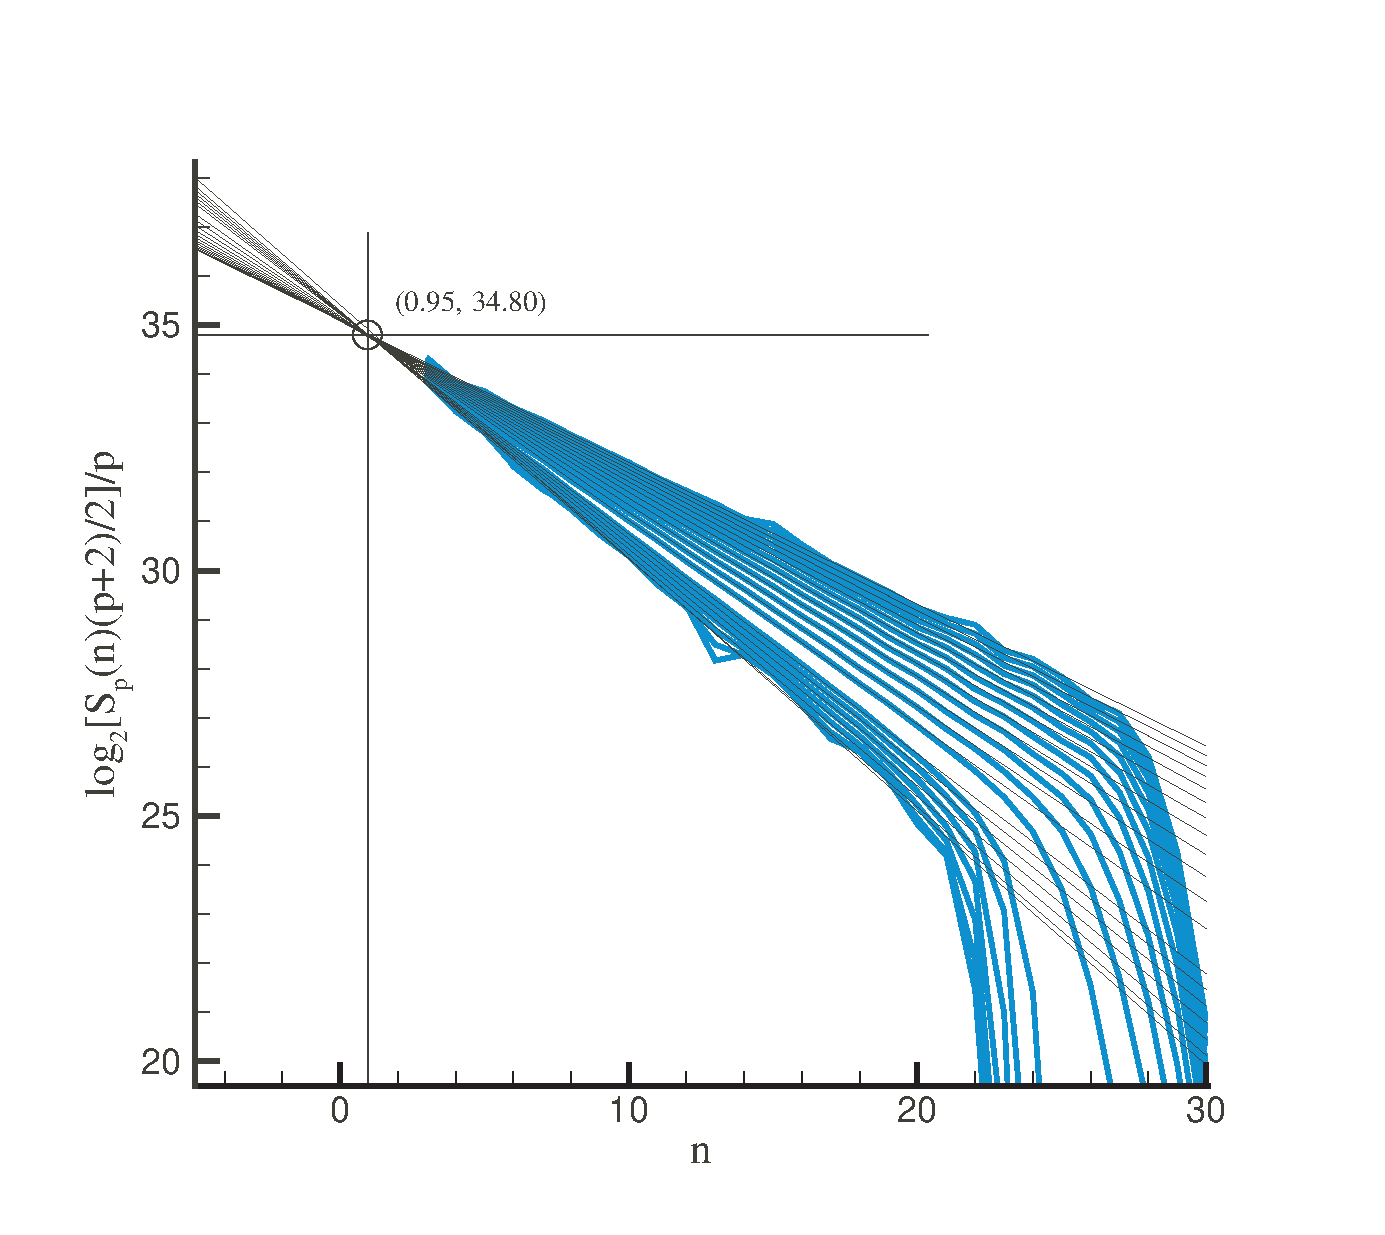
\includegraphics[width=4in]{at_focus.eps}
    \end{center}
    \caption{Rescaled structure function of Run 9 from Table \ref{table: app Sabra table} (Sabra). The functions can be formed because we have found universal coefficients.  $p = [-1.75, -1.5, \cdots, -0.5, -0.25, 0, 0.5, 1.0, \cdots, 11.5, 12.0]$} \label{fig: at focus}
\end{figure}

\subsection{The Limit of $p \rightarrow 0$}

Figure \ref{fig: at epsilon}.a show where $p = 0$ would be in the graph of rescaled structure functions.  This is due to (\ref{eq: log similarity formula 2}) involving a division by zero for $p = 0$.  Nonetheless, we can define a rescaled structure function for $p = 0$ through a limiting process.  Figure \ref{fig: at epsilon}.b clearly suggest that there are no problems for small $p$.  On the right hand side of (\ref{eq: log similarity formula 2}) it is the factor $\zeta_p/p$ that causes the problem.  Since $\zeta_0 = 0$, L'Hopitals rule can be applied.  In fact, the singularity at $p = 0$ is removable. We implement L'Hopitals rule for the data by means of a difference quotient:
\begin{equation}
    \lim_{p \rightarrow 0}\tilde{S}_p = \lim_{p \rightarrow 0}\frac{\tilde{S}_p - \tilde{S}_{-p}}{2p}.
\end{equation}
where
\begin{equation}
    \tilde{S}_p = \frac{1}{p}\ln\left(\frac{S_{p}(n)(p+2)}{2}\right).
\end{equation}

\begin{figure}[!hpt]
    \hspace{1.5in}{\centering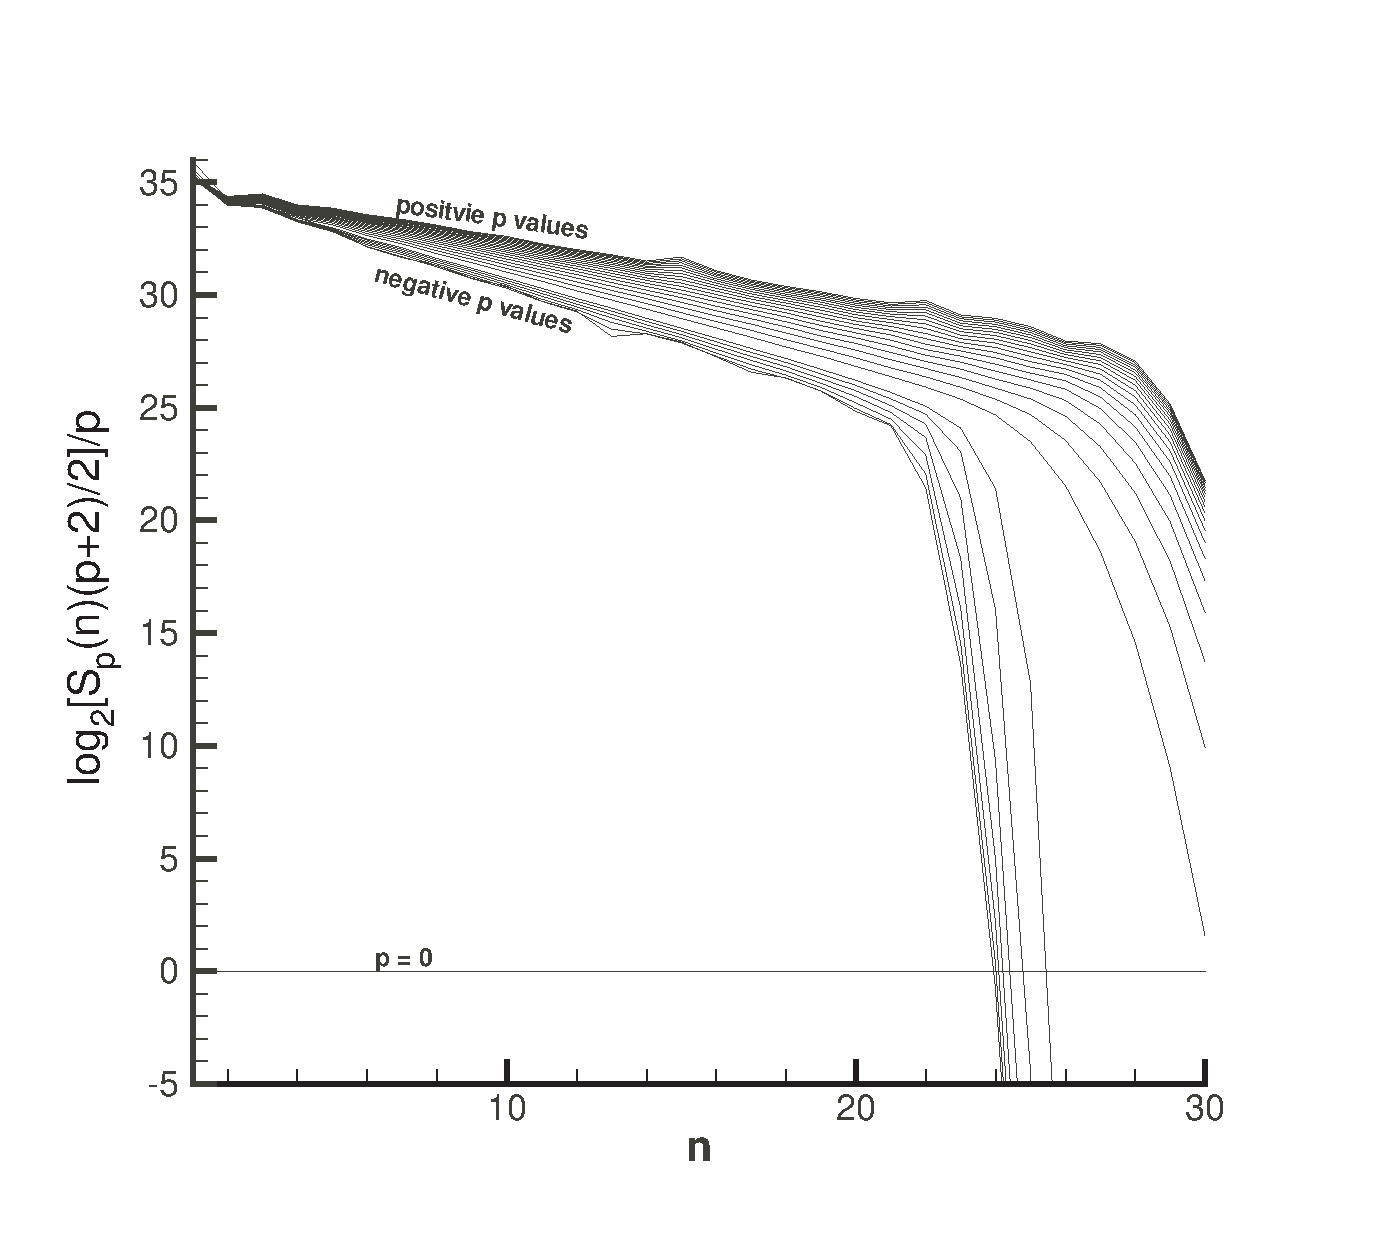
\includegraphics[width=4in]{tt_epsilon_with_0.eps}}\\

    \hspace{1.5in}{\centering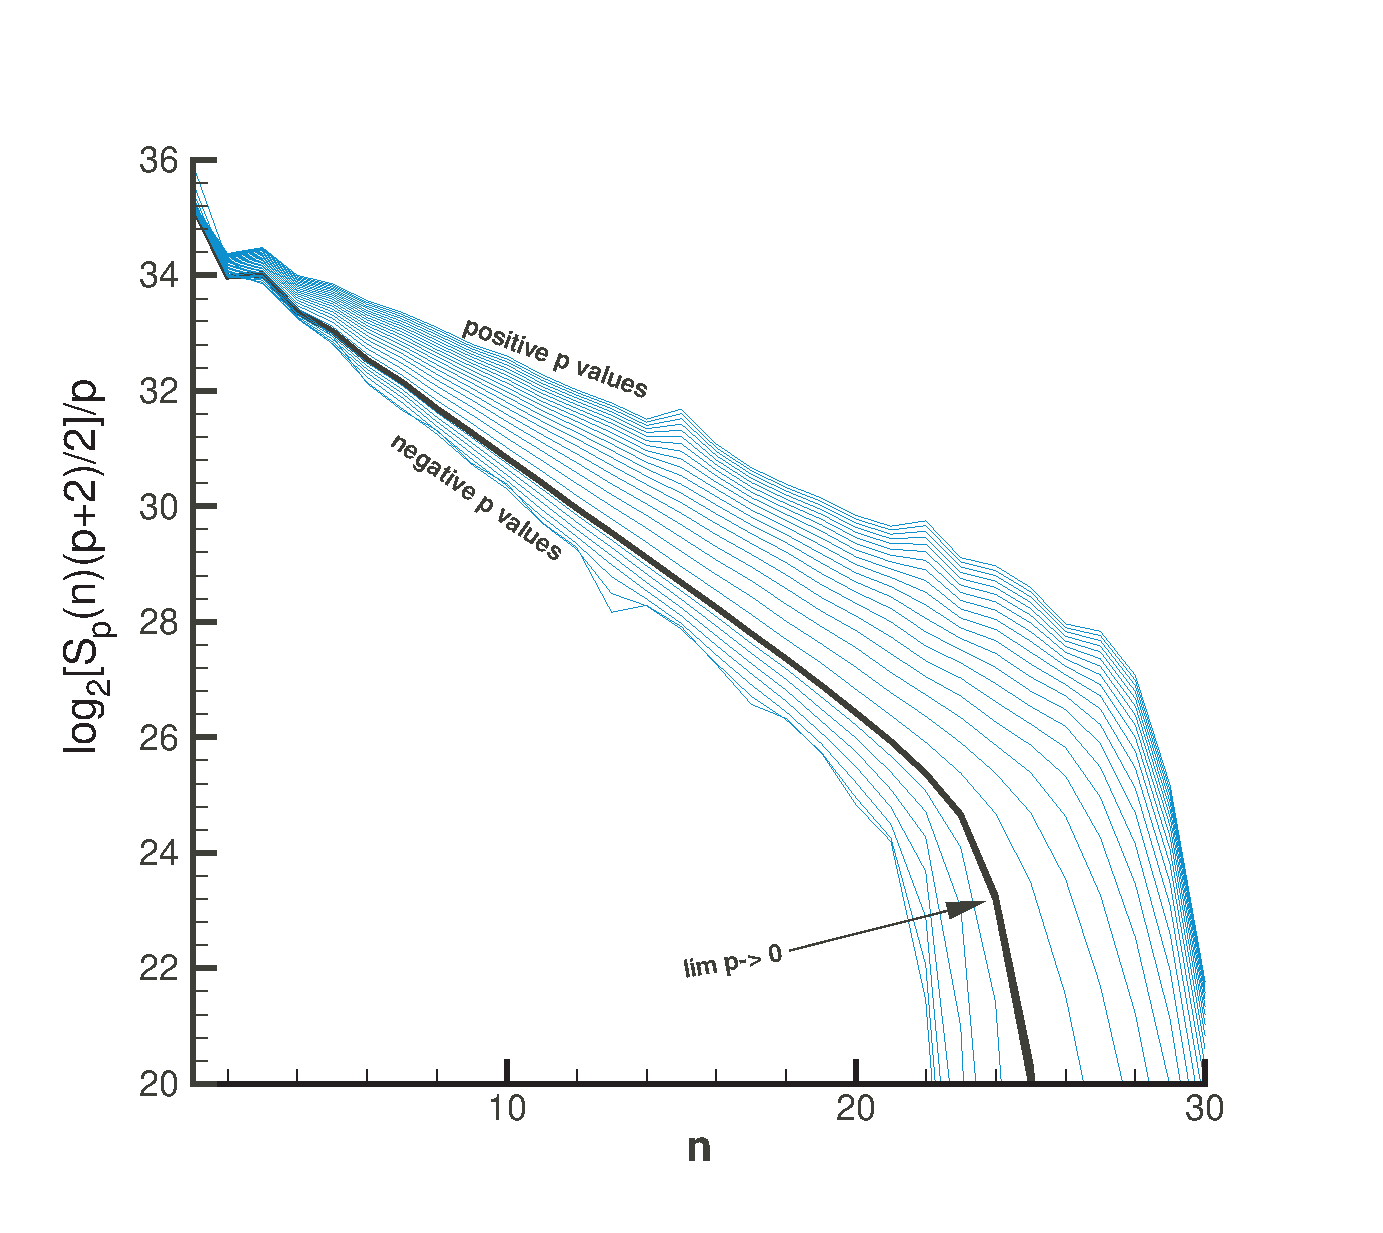
\includegraphics[width=4in]{tt_epsilon.eps}}
    \caption{Rescaled structure function of Run 9 from Table \ref{table: app Sabra table} (a) with $p = 0$ included. Note the gap between the negative and positive $p$ values. (b) as $p \rightarrow 0$  where $0.1 \geq p \geq 0.01$. Clearly a limit exists.} \label{fig: at epsilon}
\end{figure}

%\begin{equation}
%    \zeta_{p} - \frac{p}{3} = \frac{a}{3\beta(\beta-1)}\left[3(p+2)^{\beta} + (2^{\beta} - 5^{\beta})(p+2) + 2 \times5^{\beta} - 5\times2^{\beta} \right] \label{eq: Zetap}.
%\end{equation}

\vspace{2in}

\section{Graphically Measured Collapse}

Figure \ref{fig: all plots} show log-log plots of the radial profile $P_0(r;n)$ for $n$ ranging from 3 to 20.  As described in Chapter \ref{ch:self similarity of the joint pdf}, these graphs can be made to collapse by a similarity transformation.  Specifically, rigid horizontal shifts together with linear horizontal stretching.  Both shifts and stretching can be measured.  The process is as follows.  We first select one reference shell in the middle of the inertial range.  Let that be $n=12$.  The graphical objects corresponding to each of the other shells are then shifted rigidly and stretched horizontally so that the graphs match that of $P_0(r;12)$ as shown in Figures \ref{fig: s4and5with12} through \ref{fig: s19and20with12}.  Because the axes from Figure \ref{fig: all plots} are attached to $P_0(r;n)$ we can readily identify the vertical shift.  It is listed in Table \ref{table: measurements}.  We can also identify matching abscissa on the fixed and transformed scale.  The horizontal bars in Figure \ref{fig: s4and5with12} through \ref{fig: s19and20with12} are included for this purpose.  The corresponding abscissa pairs are listed in Table \ref{table: measurements}.  Since the transformation is linear only two values are needed for each $n$.  From these values we calculate the horizontal stretching factor $A$ and shift $B$, i.e.
\begin{equation}
	x_{stretched} = Ax_{f} + B
\end{equation}
Say $a$ and $b$ are two points on the fixed axis corresponding to $c$ and $d$ on the stretched axis, then
\begin{eqnarray}
	c & = & Aa + B \\
	d & = & Ab + B.
\end{eqnarray}
So that,
\begin{eqnarray}
	A & = & \frac{a-b}{c-d} \\
	B & = & \frac{bc-ad}{b-a}.
\end{eqnarray}
Figure \ref{fig: shifts} shows the vertical and horizontal shifts as functions of $n$.  We observe that both are linear functions of $n$ as called for by the theory.  The scatter around the regression line is in part due to the matching of the graphical objects being done manually.  The theory does provide analytical formulas to do a computational collapse.  However, the data we obtained contained too much statistical noise.  Therefore, we were not able to use the analytical formulas.  The vertical shift is also shown.  It forms a straight line on log-log scales.  Consequently, the stretching is a power law in $(n-n_0)$ just as predicted by the theory.  The slope is $1/\beta$ and we obtain $\beta = 1.23$ from the regression line.

\begin{table}[!htp]
    \begin{center}
    \caption{Measurements for scaling individual radial profiles.  Shell 12 is selected as the radial profile to be scaled to.  The fixed scale refers to the Shell 12 axis. The first pair of fixed and stretched scales refers to the initial alignment of the horizontal axis.  The second pair refers to the terminal alignment of the horizontal axis.}
    \begin{tabular}{||c|c|c|c|c|c||} \hline	
        \multicolumn{6}{|c|}{\emph{Measurements for Graphical Collapse}} \\ \hline \hline
        Shell & Fixed Scale & Stretched Scale & Fixed Scale & Stretched Scale & Vertical Shift \\
        \hline
        \hline
        3   &   15   &   22.2    &   21.1    &   24&     7\\
        4   &   16.2 &   22    &   22.1    &   24  &      6.2\\
        5   &   15.6 &   21    &   23.1    &   24  &      5.8\\
        6   &   16   &   21      &   22.8    &   24&      5.6\\
        7   &   14.8 &   19    &   23.2    &   24  &   3.7\\
        8   &   15.8 &   19    &   23.3    &   24  &   3.2\\
        9   &   15.6 &   18    &   23.5    &   24  &   1.8\\
        10   &   15.7&   17    &   23.6    &   24  &   1.2\\
        11   &   15.2&   16    &   23.8    &   24  &   0.8\\
        13   &   15.5&   15    &   24.3    &   24  &   -0.7\\
        14   &   17  &   15.7    &   24    &   23.6  &   -1.6\\
        15   &   17  &   15.2    &   24    &   24.3  &   -2.4\\
        16   &   18  &   15.6    &   24    &   23.3  &   -2.8\\
        17   &   18  &   15.2    &   24    &   23.1  &   -3.9\\
        18   &   19  &   16      &   24    &   22.8  &   -4.3\\
        19   &   19  &   15.1    &   24    &   22.7  &   -5.8\\
        20   &   20  &   16.1    &   24    &   22.6  &   -6.5\\
        \hline
        \hline
    \end{tabular}
    \end{center}
    \label{table: measurements}
\end{table}


\begin{figure}[!hpt]
    \begin{center}
     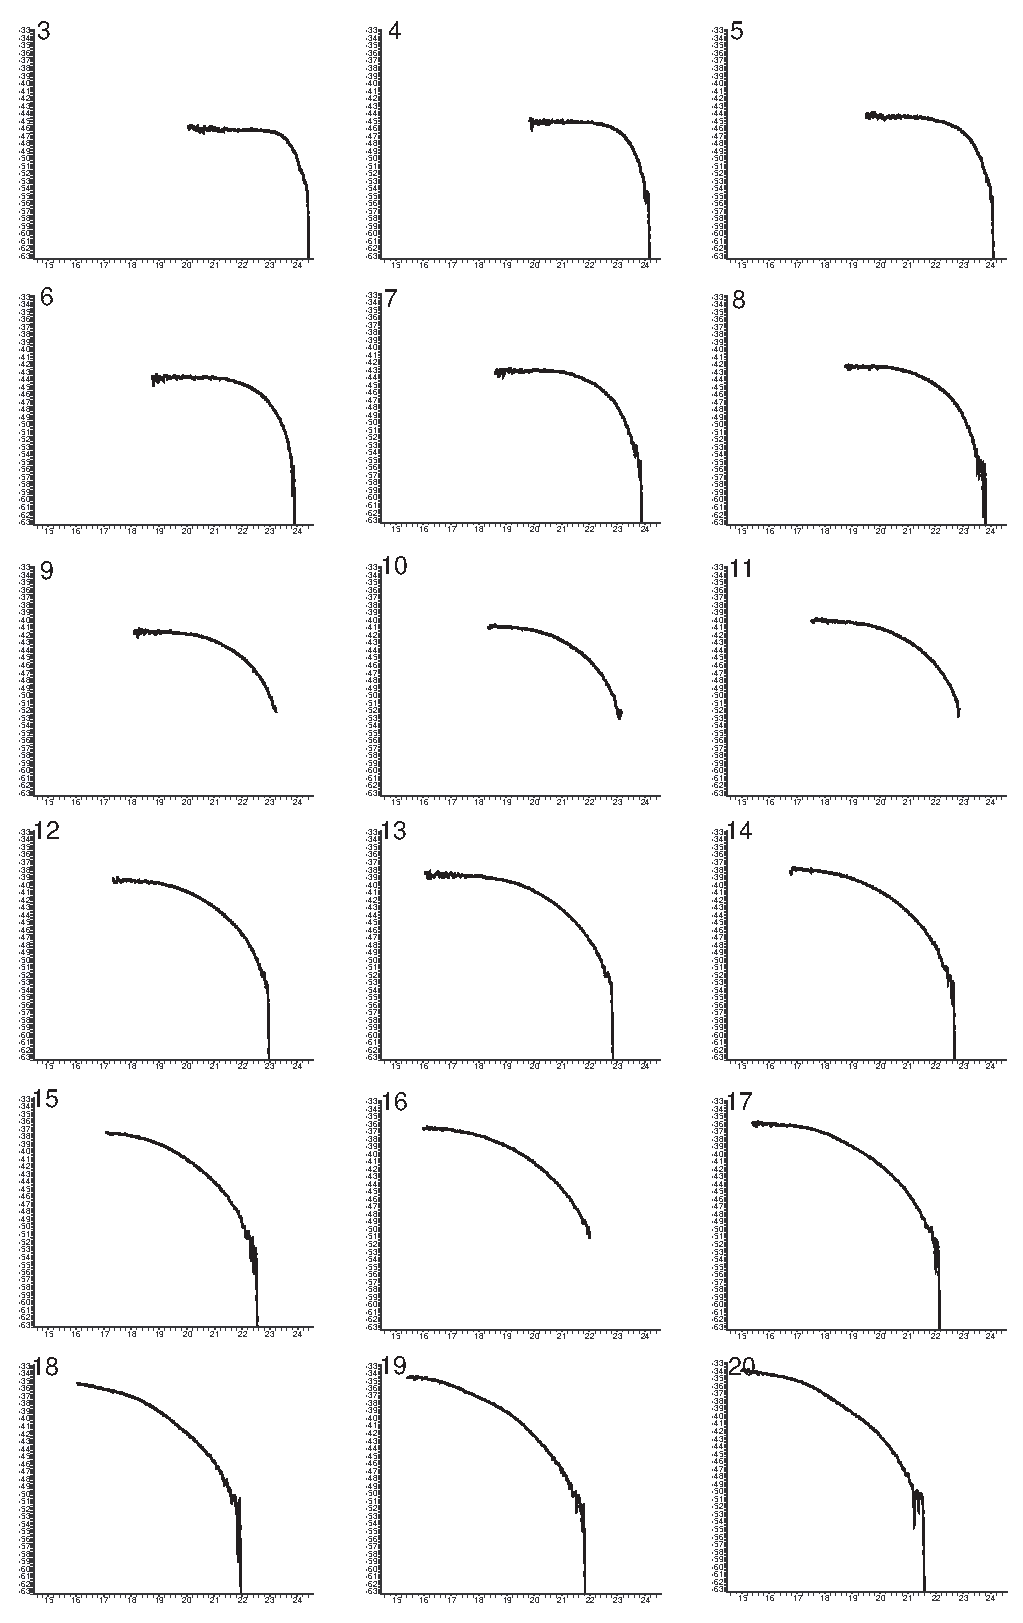
\includegraphics[width=4in]{allplots.eps}
     \end{center}
  \caption{Individual plots of each of the radial profiles that have a similar curve. The radial profiles $P_0(r;n)$ plotted on log-log scales for $3\leq n \leq 20$ for Sabra Run 9.} \label{fig: all plots}
\end{figure}

\begin{comment}
\begin{figure}[!hpt]
    \begin{center}
     \includegraphics[width=4in]{s4and5with12.eps}
     \end{center}
  \caption{(a) Collapse of $P_0(r;4)$ onto $P_0(r;12)$ using horizontal and vertical shift s together with horizontal stretching.  The vertical bars correspond to the numbers in Table (b) collapse of $P_0(r;5)$ onto $P_0(r;12)$.} \label{fig: s4and5with12}
\end{figure}

\begin{figure}[!hpt]
    \begin{center}
     \includegraphics[width=4in]{s6and7with12.eps}
     \end{center}
  \caption{(a) Collapse of $P_0(r;6)$ onto $P_0(r;12)$ (b) collapse of $P_0(r;6)$ onto $P_0(r;12)$.} \label{fig: s6and7with12}
\end{figure}

\begin{figure}[!hpt]
    \begin{center}
     \includegraphics[width=4in]{s8and9with12.eps}
     \end{center}
  \caption{(a) Collapse of $P_0(r;8)$ onto $P_0(r;12)$ (b) collapse of $P_0(r;9)$ onto $P_0(r;12)$.} \label{fig: s8and9with12}
\end{figure}

\begin{figure}[!hpt]
    \begin{center}
     \includegraphics[width=4in]{s10and11with12.eps}
     \end{center}
  \caption{(a) Collapse of $P_0(r;10)$ onto $P_0(r;12)$ (b) collapse of $P_0(r;11)$ onto $P_0(r;12)$.} \label{fig: s10and11with12}
\end{figure}

\begin{figure}[!hpt]
    \begin{center}
     \includegraphics[width=4in]{s13and14with12.eps}
     \end{center}
  \caption{(a) Collapse of $P_0(r;13)$ onto $P_0(r;12)$ (b) collapse of $P_0(r;14)$ onto $P_0(r;12)$.} \label{fig: s13and14with12}
\end{figure}

\begin{figure}[!hpt]
    \begin{center}
     \includegraphics[width=4in]{s15and16with12.eps}
     \end{center}
  \caption{(a) Collapse of $P_0(r;15)$ onto $P_0(r;12)$ (b) collapse of $P_0(r;16)$ onto $P_0(r;12)$.} \label{fig: s15and16with12}
\end{figure}

\begin{figure}[!hpt]
    \begin{center}
     \includegraphics[width=4in]{s17and18with12.eps}
     \end{center}
  \caption{(a) Collapse of $P_0(r;17)$ onto $P_0(r;12)$ (b) collapse of $P_0(r;18)$ onto $P_0(r;12)$.} \label{fig: s17and18with12}
\end{figure}

\begin{figure}[!hpt]
    \begin{center}
     \includegraphics[width=4in]{s19and20with12.eps}
     \end{center}
  \caption{(a) Collapse of $P_0(r;19)$ onto $P_0(r;12)$ (b) collapse of $P_0(r;20)$ onto $P_0(r;12)$.} \label{fig: s19and20with12}
\end{figure}

\begin{figure}[!hpt]
    \begin{center}
     \includegraphics[width=2.5in]{shifts.eps}
     \end{center}
  \caption{Graphs of (a) horizontal shift (b) vertical shift and (c) the horizontal stretching factor with regression lines fitted to the data } \label{fig: shifts}
\end{figure}

\section{Extracting the Theoretical Parameters}

In the theoretical formulas, there are four unknown constants that we must find, namely, $\beta$, $a$, $C_3$ and $n_0$. In principle, we also need $\zeta_3$, but we have already found it to be very close to one therefore, we assume $\zeta_3 \equiv 1$ in accordance with the four-fifth's law.  There are several ways to extract the constants from the data. We have seen one way of extracting $n_0$, $C_3$, and $\beta$ in sections 10.1 and 10.2. Now, we discuss two other methods for attaining these parameters.

The first involves divided differences based on the rescaled structure functions.  This method goes through step-by-step eliminating unknowns till $\beta$ is the last unknown available.  Then the method filters back through to give us values for the other unknowns.

The second method uses cumulants.  Through this method, we use ratios and graphs to determine the values.  Using both methods gives us a way to check the accuracy of the values.

\subsection{Divided Differences}

We will use two intermediate variables, $m_{p}$ and $R_{p}$.  Using these variables we will be able to extract $\beta$ which will in turn yield $a$, and we will be able to check the values of $n_{0}$ and $C_{3}$.

To find $m_{p}$, we need to rearrange (\ref{eq: log similarity formula 2}). Moving $\ln (5/2 S_{3})$ from the left and right hand side, we have
\begin{eqnarray}
    m_{p} & \equiv & \frac{3}{p}\ln\left(\frac{S_{p}(n)(p+2)}{2}\right) - \ln \left(\frac{5}{2}S_{3}\right) \nonumber\\
    & = & \ln\left(\frac{5C_{3}}{2}\right) -\frac{3}{p}\zeta_{p}(n-n_{0})\ln2 - \ln \left(\frac{5}{2}S_{3}\right) \nonumber\\
    & = & \ln\left(\frac{5C_{3}}{2}\right) -\frac{3}{p}\zeta_{p}(n-n_{0})\ln2 - \ln\left(\frac{5}{2}C_{3}2^{-\zeta_{3}(n-n_{0})}\right) \nonumber\\
    & = & \ln\left(\frac{5C_{3}}{2}\right) -\frac{3}{p}\zeta_{p}(n-n_{0})\ln2 - \ln\left(\frac{5}{2}C_{3}\right) + \zeta_{3}(n-n_{0}) \ln2 \nonumber\\
    & = & -\frac{3}{p}\zeta_{p}(n-n_{0})\ln2  + \zeta_{3}(n-n_{0}) \ln2
\end{eqnarray}
or, with $\zeta_3 = 1$:
\begin{equation}
    m_p =  \left(1-\frac{3}{p}\zeta_{p}\right)(n-n_{0})\ln2. \label{eq: mp}
\end{equation}
Through this process we have eliminated $C_{3}$ and are left with three unknowns. Note, theoretically $m_3 \equiv 0$.

\begin{figure}[!hpt]
    \begin{center}
    \includegraphics[width=4in]{at_mp_vs_m2.eps}
    \end{center}
    \caption{Plot of $m_p$ vs. $m_2$. Straight lines are superimposed over the different data sets. The data sets are represented by squares.} \label{fig: at mp vs m2}
\end{figure}

The theoretical expression (\ref{eq: mp}) vanishes for $n = n_0$ for all $p$ and is linear in $n - n_0$.  Consequently, $(m_2, m_p)$ constitutes a parameteric representation for a straight line with $(n - n_0)$ as the parameter.  This line passes through (0,0) regardless of the value of $p$.

Figure \ref{fig: at mp vs m2} shows $m_{p}$ vs. $m_{2}$. We substitute in the regression line values we found previously for $\zeta_p$.  Using this figure, the power laws are tested once more.  The straight lines through the points are a clear indication that the power laws do hold.  Note, that all lines meet at $(0,0)$. Thus, the ratio of $m_{p}$ and $m_{2}$ is independent of $n-n_{0}$ in the power law regime, i.e.
\begin{equation}
    \frac{m_{p}}{m_{2}} = \frac{\left(1-\frac{3}{p}\zeta_{p}\right)(n-n_{0})\ln2}{\left(1-\frac{3}{2}\zeta_{2}\right)(n-n_{0})\ln2}.
\end{equation}
This eliminates $n_{0}$ from the equation. We will call the reduced ratio $R_p$, i.e.
\begin{equation}
    R_p =  \frac{\left(1-\frac{3}{p}\zeta_{p}\right)}{\left(1-\frac{3}{2}\zeta_{2}\right)} \label{eq: rp in process}
\end{equation}

Next, we substitute the expressions for $\zeta_{p}$ and $\zeta_{2}$ into (\ref{eq: rp in process}). In doing so, we find that $R_p$ is independent of $a$,
\begin{eqnarray}
     R_{p} & = & \frac{\frac{a}{p\beta(\beta-1)}\left(3(p+2)^{\beta} + (2^{\beta}-5^{\beta})(p+2) + 2\times5^{\beta}-5\times2^{\beta}\right)}{\frac{a}{2\beta(\beta-1)}\left(3(2+2)^{\beta} + (2^{\beta}-5^{\beta})(2+2) + 2\times5^{\beta}-5\times2^{\beta}\right)} \nonumber\\
     & = & \frac{2\left(3(p+2)^{\beta} + (2^{\beta}-5^{\beta})(p+2) + 2\times5^{\beta}-5\times2^{\beta}\right)}{p\left(3\times4^{\beta} - 2^{\beta}-2\times5^{\beta}\right)}. \label{eq: rp}
\end{eqnarray}
$R_{p}$ is an expression that can be computed from the data for each value of $n$; see Figure \ref{fig: at rp}. The expression should theoretically be independent of $u$. As one would expect, the larger $p$ becomes the more statistical noise we observe.

\begin{figure}[!hpt]
    \begin{center}
    \includegraphics[width=4in]{at_rp.eps}
    \end{center}
    \caption{\ref{eq: rp} for $5\geq n \geq 20$.} \label{fig: at rp}
\end{figure}

In principle, (\ref{eq: rp}) should allow us to solve for $\beta$. In order to determine $\beta$, we first average each $R_{p}$ over $n$.  After this, we determine the different standard deviations which gives a measure for the statistical noise.  Once done, we can plot various values of $\beta$, restricted to $0<\beta<3$.  Given the average $R_{p}$ and the standard deviation of $R_{p}$, we can estimate the $\beta$ value that best matches the data.  We find $\beta \simeq 1.6$.

\begin{figure}[!hpt]
    \begin{center}
        \includegraphics[width=4in]{at_ave_rp.eps}
    \end{center}
    \caption{Average $R_p$ with standard deviation as error bars.  Surrounding curves are different values of $\beta$ computed to find the best fit.}  \label{fig: at average rp beta}
\end{figure}

Now that we know $\beta$ we can find $a$ from (\ref{eq: mp}).  If we define
\begin{equation}
    K_{p} = \frac{1}{a}\left(\zeta_{p} - \zeta_{3}\frac{p}{3}\right)
\end{equation}
then
\begin{eqnarray}
    m_{p} & = & \left(\frac{3}{p}\zeta_{p} - 1\right)(n-n_0)\ln2 \nonumber \\
    & = & \left(\frac{3}{p}\left(aK_{p} + \frac{p}{3}\right) - 1\right)(n-n_0)\ln2 \nonumber \\
    & = & \frac{3}{p}aK_{p}(n-n_0)\ln2.
\end{eqnarray}
Therefore,
\begin{equation}
    a = \frac{m_{p}p}{3K_{p}(n-n_0)\ln2}. \label{eq: a}
\end{equation}
For $\beta = 1.6$, we find $a = -0.11$.

\begin{figure}[!htp]
    \begin{center}
        \includegraphics[width = 4in]{at_find_a_beta_160.eps}
    \end{center}
    \caption{Using the value we find in (\ref{eq: rp}), we plug into (\ref{eq: a}).  The slope of the inertial range yields the value of $a$.}
\end{figure}

\subsection{Cumulants}

Another technique to determine the four parameters in the similarity theory is to utilize cumulants. While moments are generated from a series expansion of the first characteristic function the Fourier transform of the pdf, cumulants are are generated from the second characteristic function. Specifically, suppose we have a random variable $-\infty < X < \infty$ with a pdf $f(x)$ then the Fourier transform of $f$ is the first characteristic function
\begin{equation}
	\hat{F}(s) = \int^{\infty}_{-\infty}f(x)e^{isx}dx \label{eq: fourier transform}
\end{equation}
This function has a MacLaurin series which one finds by expanding the exponential function $e^{isx}$,
\begin{eqnarray}
	\hat{F}(s) & = & \int^{\infty}_{-\infty} f(x) \sum^{\infty}_{k = 0}\frac{(isx)^k}{k!}dx \nonumber \\
	& = & \sum^{\infty}_{k = 0}\frac{(is)^k}{k!}\int^{\infty}_{-\infty} x^k f(x)dx \nonumber \\
	& = & \sum^{\infty}_{k = 0}\frac{(is)^k}{k!}\mathcal{M}_k,
\end{eqnarray}
where $\mathcal{M}_k = \langle X^k \rangle$ are the moments.  The second characteristic function is then defined as
\begin{equation}
	\hat{G}(s) = \log \left(\hat{F}(s)\right).
\end{equation}
Its expansion reads
\begin{equation}
	\hat{G}(s) = \sum^{\infty}_{k = 0}Q_k \frac{(is)^k}{k!} \label{eq: cumulant series}
\end{equation}
where the coefficients, $Q_k$ are called the cumulants of the random variable, $X$, or the pdf, $f$.

\vspace{2in}

\subsubsection{Defining Cumulants}

The cumulants, $Q_k$, are related to moments through formulas that can be found in \cite{Kendall69}. We use the first three of these formulas
\begin{eqnarray}
    Q_{1} \equiv \langle\langle X \rangle\rangle & = & \langle X \rangle \label{eq: Q1 theory} \\
    Q_{2} \equiv \langle\langle X^2 \rangle\rangle & = & \langle X^2 \rangle - \langle X \rangle^{2} \label{eq: Q2 theory} \\
    Q_{3} \equiv \langle\langle X^3 \rangle\rangle & = & \langle X^3 \rangle - 3\langle X^2 \rangle\langle X \rangle + 2\langle X \rangle^{3} \label{eq: Q3 theory}.
\end{eqnarray}

These formulas show how we can compute the cumulants from computational data i.e., the moments of $X$.  From (\ref{eq: cumulant series}) follows
\begin{equation}
    Q_k \equiv \left.\left[(-i)^k\left(\frac{d}{ds}\right)^{k}\hat{G}(s)\right]\right|_{s = 0}. \label{eq: cumulant def}
\end{equation}
Let us define the pdf for the shell amplitude, $A$, as $\phi$, i.e.,
\begin{equation}
    \phi(x)dx = Pr\{x\leq A\leq x+ dx\}.
\end{equation}
Moreover, let $\psi$ be the pdf for $\ln A$, i.e.,
\begin{equation}
    \psi(y)dy = Pr\{y\leq \ln A\leq y+ dy\}.
\end{equation}
There is, of course, a relationship between $\phi$ and $\psi$.  We found it previously in Chapter \ref{ch:self similarity of the joint pdf}, namely
\begin{equation}
    \phi(x) = \frac{\psi(\ln x)}{x}.
\end{equation}
By a change of variables,  $x = e^{t}$, we obtain $\psi$ in terms of $\phi$:
\begin{equation}
    \psi(t) = e^t \phi(e^t).
\end{equation}
The characteristic function of $\hat{\Psi}$ is then obtained through a Fourier integral as follows:
\begin{eqnarray}
    \hat{\Psi}(s) & = & \int^{\infty}_{-\infty}\psi(x)e^{isx}dx \nonumber \\
    & = & \int^{\infty}_{-\infty}e^x\phi(e^x)e^{ixs}dx \nonumber \\
    & = & \int^{\infty}_{-\infty}\phi(e^x)e^{(is+1)x}dx .
\end{eqnarray}
By substitution $u = e^x$ and $du = e^xdx$, we can express $\hat{\Psi}(s)$ as a Mellin transform, i.e.,
\begin{eqnarray}
    \hat{\Psi}(s) & = & \int^{\infty}_{0}\phi(u)u^{is}du \nonumber \\
    & = & \int^{\infty}_{0}\phi(u)u^{is+1}\frac{du}{u} \nonumber \\
    & = & \mathcal{M}[\phi(u); is + 1].
\end{eqnarray}
The Mellin transform of $\phi$ brings us back to the power laws for the inertial range,
\begin{equation}
     \hat{\Psi}(s) = S_{is}(\ell) =  C_{is}\ell^{\zeta_{is}}. \label{eq: at cap psi}
\end{equation}
We notice that the order index $p$, i.e. in $C_p$ and $\zeta_p$, is now replaced by the complex value $is$.  Thus, for (\ref{eq: at cap psi}) to be of use, we must have analytic formulas for $C_p$ and $\zeta_p$.  Otherwise, we cannot extend $C_p$ and $\zeta_p$ into the complex plane. The theory from Chapter \ref{ch:a new theory} is helpful in this regard.

\subsubsection{Applying Cumulants}

It follows from (\ref{eq: at cap psi}) that
\begin{equation}
    \ln \hat{\Psi}(s) = \ln C_{is} + \zeta_{is}\ln \ell
\end{equation}
where the expansion
\begin{equation}
    \ln \hat{\Psi}(s) = \sum^{\infty}_{k = 0}Q_k\frac{(is)^k}{k!}
\end{equation}
provides the cumulants of $\ln A_n$.

Using our previous shell notation (\ref{eq: new sfp}) we have
\begin{equation}
    \hat{\Phi}_{n}(s) = \mathcal{M}\left[\phi_{n}(u);is+1\right] = S_{is}(n) = C_{is}2^{-\zeta_{is}(n-n_{0})}. \label{eq: psi which is sfp}
\end{equation}
For simplicity, let $\eta = (n-n_{0})\ln 2$, so that (\ref{eq: psi which is sfp}) reads
\begin{equation}
    S_{is}(n) = C_{is}e^{-\eta\zeta_{is}} . \label{eq: psi with eta}
\end{equation}
Then, using (\ref{eq: cumulant series}), (\ref{eq: cumulant def}), and (\ref{eq: psi which is sfp}), we obtain
\begin{equation}
    Q_m = \left.\left[\left(-i\frac{d}{ds}\right)^{m}\left(\ln C_{is} - \eta\zeta_{is}\right)\right]\right|_{s = 0},
\end{equation}
which clearly shows that all cumulants are linear functions of $\eta$ in the inertial range.

The first cumulant, $m=1$, is
\begin{eqnarray}
    Q_{1} & \equiv & \left.\left[\left(-i\frac{d}{ds}\right)^{1}\ln \left(C_{is}e^{-\eta\zeta_{is}}\right)\right]\right|_{s = 0} \nonumber \\
    & = & \left.\left[-i\left(\frac{iC_{is}'}{C_{is}} - i\eta\zeta_{is}'\right)\right]\right|_{s=0} \nonumber \\
    & = & \left.\left[\frac{C_{is}'}{C_{is}} - \eta\zeta_{is}'\right]\right|_{s=0} .
\end{eqnarray}
Since $C_0 \equiv 1$, we obtain
\begin{equation}
    Q_{1} =  C_{0}' - \eta\zeta_{0}' .
\end{equation}
Using the same process, we find $Q_{2}$,
\begin{eqnarray}
    Q_{2} & \equiv & \left.\left[\left(-i\frac{d}{ds}\right)^{2}\ln \left(C_{is}e^{-\eta\zeta_{is}}\right)\right]\right|_{s = 0} \nonumber \\
    & = & \left.\left[-i\left(\frac{iC_{is}C_{is}'' - iC_{is}'^{2}}{C_{is}^{2}} - i\eta\zeta_{is}''\right)\right]\right|_{s=0} \nonumber \\
    & = & \left.\left[\frac{C_{is}C_{is}'' - C_{is}'^{2}}{C_{is}^{2}} - \eta\zeta_{is}''\right]\right|_{s=0} .
\end{eqnarray}
Again, using $C_0 \equiv 1$, we have
\begin{equation}
    Q_{2} =  C_{0}'' - C_{0}'^{2} - \eta\zeta_{0}'' .
\end{equation}
For $Q_{3}$,
\begin{eqnarray}
    Q_{3} & \equiv & \left.\left[\left(-i\frac{d}{ds}\right)^{3}\ln \left(C_{is}e^{-\eta\zeta_{is}}\right)\right]\right|_{s = 0} \nonumber \\
    & = & \left.\left[-i\left(\frac{iC_{is}C_{is}'''-iC_{is}''C_{is}'}{C_{is}^{2}} - 2i\frac{C_{is}^{2}C_{is}''-C_{is}'^{3}}{C_{is}^{4}} - i\eta\zeta_{is}'''\right)\right]\right|_{s=0} \nonumber \\
    & = & \left.\left[\frac{C_{is}C_{is}'''-C_{is}''C_{is}'}{C_{is}^{2}} - 2\frac{C_{is}^{2}C_{is}''-C_{is}'^{3}}{C_{is}^{4}} - \eta\zeta_{is}'''\right]\right|_{s=0} \nonumber \\
    & = &=  C_{0}'''-C_{0}''C_{0}' - 2\left(C_{0}''-C_{0}'^{3}\right) - \eta\zeta_{0}''' .
\end{eqnarray}

Using the theoretical formulas for $\zeta_p$ and $C_p$ from \cite{Melander2007} we calculate the derivatives $C_{0}^{(m)}$ and $\zeta_{0}^{(m)}$. As a result we have the cumulants expressed in term of the parameters $a$, $\beta$, $C_3$, and $n_0$,
\begin{equation}
    Q_{1} = -\frac{1}{2} + \frac{1}{3}\ln \left(\frac{5}{2}C_{3}\right) -  \left(\frac{a}{3\beta(\beta-1)}  \left(\frac{5}{2}\beta2^{\beta}+2^{\beta}-5^{\beta}\right)+\frac{1}{3}\right)(n-n_{0})\ln2, \label{eq: Q1}
\end{equation}
\begin{equation}
    Q_{2} = \frac{1}{4}-\frac{1}{4}a2^{\beta}(n-n_{0})\ln2, \label{eq: Q2}
\end{equation}
and
\begin{equation}
    Q_{3} = -\frac{1}{4}-\frac{1}{8}a2^{\beta}(\beta-2)(n-n_{0})\ln2. \label{eq: Q3}
\end{equation}

Note that $Q_1$ and $Q_2$ define all four parameters.  The higher orders do not bring any new information, but also do not contradict $Q_1$ and $Q_2$ \cite{Kendall69}. We rearrange cumulant formulas for easier graphical interpretation as follows
\begin{equation}
    3Q_{1} + \frac{3}{2} = \ln \left(\frac{5}{2}C_{3}\right) -  \left(\frac{a}{\beta(\beta-1)}  \left(\frac{5}{2}\beta2^{\beta}+2^{\beta}-5^{\beta}\right)+1\right)(n-n_{0})\ln2, \label{eq: 3Q1 p 3o2}
\end{equation}
\begin{equation}
    4Q_{2} - 1 = a2^{\beta}(n-n_{0})\ln2, \label{eq: 4Q2 m 1}
\end{equation}
and
\begin{equation}
    8Q_{3} + 2 = -a2^{\beta}(\beta-2)(n-n_{0})\ln2. \label{eq: 8Q3 p 2}
\end{equation}

The moment based cumulant formulas, i.e. (\ref{eq: Q1 theory}), (\ref{eq: Q2 theory}), (\ref{eq: Q3 theory}), with $X = \ln A_n$ and the derived cumulant formulas, i.e. (\ref{eq: Q1}), (\ref{eq: Q2}), (\ref{eq: Q3}) describe the same set of statistics.  We can calculate the moment based cumulants from the data to get the left hand sides of (\ref{eq: 3Q1 p 3o2}), (\ref{eq: 4Q2 m 1}), (\ref{eq: 8Q3 p 2}).  By extracting the regression lines, we can obtain the four unknown constants, $a$, $\beta$, $C_3$, and $n_0$.  Figure \ref{fig: at cumulant} displays the cumulants and their respective regression lines. Graphically, we find the value of $n_0$ by inspecting the zero crossings of $4Q_2 - 1$ and $8Q_3 + 2$. The former being statistically more accurate then the latter.

\begin{figure}[!hpt]
    \begin{center}
    \includegraphics[width=4in]{at_cumulant.eps}
    \end{center}
    \caption{Equations (\ref{eq: 3Q1 p 3o2}), (\ref{eq: 4Q2 m 1}), (\ref{eq: 8Q3 p 2}) plotted along with their respective regression lines.} \label{fig: at cumulant}
\end{figure}

The regression lines for the derived cumulant formulas can be written as
\begin{equation}
    Q_m = A_m + (n-n_0)B_m
\end{equation}
yields (\ref{eq: Q1}), (\ref{eq: Q2}), and (\ref{eq: Q3}). The data, i.e. Figure \ref{fig: at cumulant},
\begin{eqnarray}
    \tilde{Q}_{1} = 3Q_1 + \frac{3}{2} & = & \tilde{A}_{1} + n\tilde{B}_{1}  \\
    \tilde{Q}_{2} = 4Q_2 - 1 & = & \tilde{A}_{2} + n\tilde{B}_{2} \label{eq: 4q2} \\
    \tilde{Q}_{3} = 8Q_3 + 2 & = & \tilde{A}_{3} + n\tilde{B}_{3}  .
\end{eqnarray}
corresponding to (\ref{eq: 3Q1 p 3o2}), (\ref{eq: 4Q2 m 1}), and (\ref{eq: 8Q3 p 2}). While we may not know the specific values of $A_m$, $B_m$, we do know the values of $\tilde{A}_m$, $\tilde{B}_m$.

Now, we determine the ratios between $B_m$ and $\tilde{B}_m$. Starting with $m = 1$, we have
\begin{eqnarray}
    3Q_{1} + \frac{3}{2} & = & 3A_{1} + 3B_{1}(n-n_{0}) + \frac{3}{2} \nonumber \\
    & = & 3A_{1} + 3B_{1}n - 3B_{1}n_{0} + \frac{3}{2} = \tilde{A_{1}} + \tilde{B_{1}}n. \label{eq: 3Q1 p 3o2 with tildes}
\end{eqnarray}
Hence, $\tilde{B_{1}} = 3B_{1}$. We proceed to find the relationship between $\tilde{B_{2}}$ and $B_{2}$,
\begin{eqnarray}
    4Q_{2} - 1 & = & 4A_{2} + 4B_{2}(n-n_{0}) - 1 \nonumber \\
    & = & 4A_{1} + 4B_{2}n - 4B_{2}n_{0} - 1 = \tilde{A_{2}} + \tilde{B_{2}}n. \label{eq: 4Q2 m 1 with tildes}
\end{eqnarray}
Then, $\tilde{B_{2}} = 4B_{2}$. The relationship between $\tilde{B_{3}}$ and $B_{3}$ follows the previous steps. We find $\tilde{B_{3}} = 8B_{3}$. Now, we have all the equations and ratios we need to solve for the unknown constants.

\subsubsection{Solving for Parameters}

First, we will calculate $n_{0}$.  To accomplish this, we use (\ref{eq: 4Q2 m 1}) to obtain
\begin{equation}
    4Q_{2}(n_{0}) - 1 = -a2^{\beta}(n_{0}-n_{0})\ln 2  \label{eq: to go below}
\end{equation}
such that combing (\ref{eq: 4q2}) with (\ref{eq: to go below}) yields
\begin{equation}
    \tilde{A_{2}} + \tilde{B_{2}}n_{0} = 0
\end{equation}
\begin{equation}
    n_{0} = \frac{-\tilde{A_{2}}}{\tilde{B_{2}}}. \label{eq: found n0}
\end{equation}
Using the numerical values from the linear fits in Figure \ref{fig: at cumulant} for $\tilde{A}_2$ and $\tilde{B}_2$, we obtain $n_0 = 1.12$.

To find $C_{3}$, we use the same process with (\ref{eq: 3Q1 p 3o2}) and (\ref{eq: 3Q1 p 3o2 with tildes}). Letting $n = n_{0}$, we have
\begin{equation}
    3Q_{1}(n_{0}) + \frac{3}{2} = \ln \left(\frac{5}{2}C_{3}\right)
\end{equation}
then,
\begin{equation}
    \ln \left(\frac{5}{2}C_{3}\right) = \tilde{A_{1}} + \tilde{B_{1}}n_{0}
\end{equation}
so that
\begin{equation}
    C_{3} = \frac{2}{5}e^{\tilde{A_{1}} + \tilde{B_{1}}n_{0}} . \label{eq: found C3}
\end{equation}
Substituting in the numerical values for $\tilde{A}_1$ and $\tilde{B}_1$ along with the value we found for $n_0$, we find $C_3 =  0.84 \times 10^{31}$. Note this enormous value of $C_3$ is a consequences of the way we non-dimensionalized the shell model in Chapter \ref{ch:shell models}.  Essentially, we scaled our viscous unit by setting $\nu = 1$ and having enormous forcings. We can check that this $C_{3}$ is close to the $C_{3}$ we located in the rescaled structure function graph, see Figure \ref{fig: at focus}.  However, we need to remember that the number we found there was actually $\frac{1}{3}\log_{2}C_{3} = 34.8$. Using the cumulants, we find $\frac{1}{3}\log_{2}C_{3} = 34.2$. We do indeed find the values similar.

Next, we would like to find $a$ and $\beta$.  From (\ref{eq: 4Q2 m 1 with tildes}), we have
\begin{equation}
    4B_{2} = \tilde{B_{2}},
\end{equation}
so that
\begin{equation}
    4\left(\frac{-1}{4}a2^{\beta}\ln 2\right) = \tilde{B_{2}},
\end{equation}
and consequently,
\begin{equation}
    a = \frac{-\tilde{B_{2}}}{2^{\beta}\ln2} . \label{eq: found a}
\end{equation}
Now, we will substitute (\ref{eq: found a}) into $\tilde{B_{1}} = 3B_{1}$ from (\ref{eq: 3Q1 p 3o2 with tildes}). Solving for $\beta$, we obtain
\begin{eqnarray}
    \tilde{B_{1}} & = &   - 3\left(\frac{a}{3\beta(\beta-1)} \left(\frac{5}{2}\beta2^{\beta}+2^{\beta}-5^{\beta}\right)+\frac{1}{3}\right)\ln2  \nonumber \\
    & = & - \left(\frac{-\tilde{B_{2}}}{2^{\beta}\ln2}\cdot\frac{1}{\beta(\beta-1)} \left(\frac{5}{2}\beta2^{\beta}+2^{\beta}-5^{\beta}\right)+1\right)\ln2 \label{eq: found beta}
\end{eqnarray}
To solve for $\beta$, let us turn (\ref{eq: found beta}) into a function based solely on $\beta$.
\begin{equation}
    F(\beta) =  - \left(\frac{-\tilde{B_{2}}}{2^{\beta}\ln2}\cdot\frac{1}{\beta(\beta-1)} \left(\frac{5}{2}\beta2^{\beta}+2^{\beta}-5^{\beta}\right)+1\right)\ln2 - \tilde{B_{1}}
\end{equation}
The value of $\beta$ we are interested in is the root of $f(\beta) = 0$. This value is $\beta = 1.36$, see Figure \ref{fig: at f of beta}. We then take this $\beta$ value and substituting into (\ref{eq: found a}) to solve for $a$, we find $a = -0.13$

\begin{figure}[!hpt]
    \begin{center}
    \includegraphics[width=4in]{at_fofbeta.eps}
    \end{center}
    \caption{$F(\beta)$ solving for $f(\beta) = 0$. The root is $\beta = 1.3558$.} \label{fig: at f of beta}
\end{figure}

Ratios between higher order cumulant $Q_m$, $m \geq 2$ depend on $\beta$.  So, in principle $\beta$ is determined uniquely by the higher orders, but the statistical noise amplifies quickly as the order increases. As an illustration, we can check the value of $\beta$ by using the ratio of $Q_{2} - \frac{1}{4}$ to $Q_{3} + \frac{1}{4}$,
\begin{eqnarray}
    \frac{Q_{3} + \frac{1}{4}}{Q_{2} - \frac{1}{4}} & = & \frac{-\frac{1}{8}a2^{\beta}(\beta-2)(n-n_{0})\ln2}{-\frac{1}{4}a2^{\beta}(n-n_{0})\ln 2} \nonumber \\
    & = & \frac{\beta}{2} - 1 \nonumber \\
    \Rightarrow \beta & = & 2\left(\frac{Q_{3} + \frac{1}{4}}{Q_{2} - \frac{1}{4}} + 1\right) \label{eq: ratio solving for beta}
\end{eqnarray}
Here the right hand side should be independent of the shell number $n$ provided that the statistics have convergent and we are in the inertial range.  Graphically, we can examine (\ref{eq: ratio solving for beta}) three ways as illustrated by Figure \ref{fig: at ratio cumulants}.  The obvious route is to observe what the ratio looks like through the use of our cumulant data from (\ref{eq: 3Q1 p 3o2}), (\ref{eq: 4Q2 m 1}), (\ref{eq: 8Q3 p 2}), see Figure \ref{fig: at cumulant}.  This gives a rather jagged curve which does not give a clear indication of the value of $\beta$.  The next method we implement is the regression line data for $Q_2$ and $Q_3$. The result is a smooth curve with a spike at small $n$ but as $n$ increases the curve levels off at about 1.66.  The last technique we employ is a minmax method with the regression data.  This gives almost no fluctuation and a $\beta$ value of about 1.64.

\begin{figure}[!hpt]
    \begin{center}
    \includegraphics[width=4in]{at_ratio_cumulants.eps}
    \end{center}
    \caption{Ratio (\ref{eq: ratio solving for beta}) to solve for $\beta$.} \label{fig: at ratio cumulants}
\end{figure}

\section{Results}

We have used several different techniques to find $a$, $\beta$, $C_3$, and $n_0$.  We did expect $a<0$ and $1<\beta<2$ and found this to be true in each case \cite{Melander2007}.  While using rescaled regression lines yielded $n_0$ and $C_3$, graphically measuring only produced one constant, $\beta$.  Divided differences and cumulants, on the the other hand,  were methods that supplied us with all four values. While each method produced varying values, the values were approximately the same.

\end{comment} 
   %Chapter) Applying the Theory
%\chapter{Conclusion} \label{ch:conclusion}



%===================================================================
%   Appendices go here if no appendix, remove \StartAppendix
%===================================================================
%\StartAppendix %All chapters from this point are treated as appendices

%
\chapter{APPENDIX} \label{ch:table appendix}

\vspace{-0.2in}

\section{Description of GOY Shell Model Runs and Table}

In most cases, we have forced the models in the first shell so that the inertial range forms on the ultraviolet side.  However, in run 2 from Table \ref{table: app GOY table}, we force in shell seven and observe an infra-red inertial range form.  Run 1 uses the parameters of \cite{Yamada} originally used.  This run is used as a control and to reproduce Pisarenko et. al. \cite{Pisarenko} work.  Run 2 is equivalent to Run 1 as far as the parameters are concerned.  However, in this run, we force in shell 6.  As a result, we see an infra-red inertial range.  We can apply the affine collapse to this data as well. This result is of interest in the light of Carl Gibson idea that the true cascade in turbulence is from small to large scales \cite{Gibson}. We start with small forcing in Run 3.  Here, the forcing is small enough that the solution is quasi-periodic and we have no inertial range.  We can observe this in the distribution of $u_n$.  In this particular case, the points were located in a ring that was centered at the origin (see Figure \ref{fig: circ symtrc}).   However, there is still circular symmetry about the origin in this case.

\begin{figure}[!htp]
    \begin{center}
        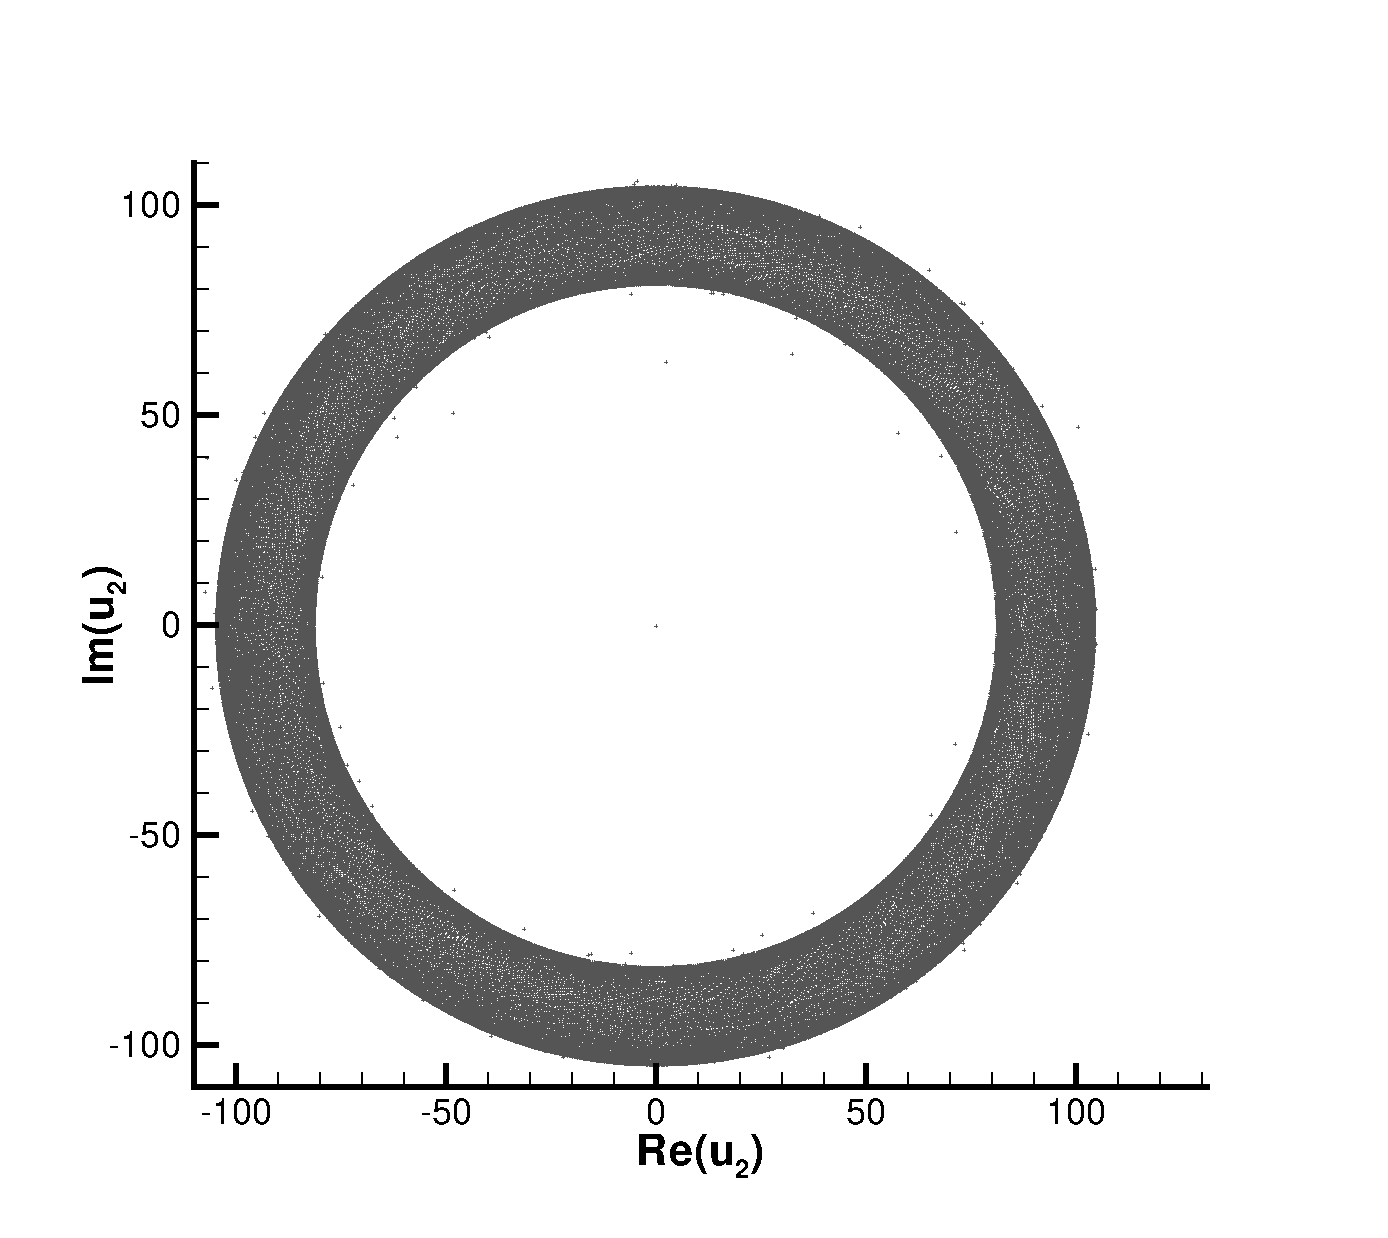
\includegraphics[width=4in]{ns_run10urui.eps}
    \end{center}
    \caption{Distribution of $u_i$. This plot displays the quasi-periodic nature of Run 3 for shell 10 (eps file).} \label{fig: circ symtrc}
\end{figure}

In order to obtain an inertial range which the new similarity theory requires, we increase the forcing for Run 4.  In Run 4, we still have virtually no inertial range.  We must increase the forcing further.  In Run 5, the model is chaotic and we have somewhat more of an inertial range.  Run 6 increases the forcing and the shell number, however we are not obtaining enough of an inertial range. In Run 7, we increase the forcing significantly.  The number of shells remains the same, but this time, we observe a distinct inertial range.  We want to observe how much forcing we can pump into the system before numerical problems arise.  Thus, we create Run 8 and Run 9.  Run 10 is at the limit of what is numerically possible with out model.  This run took four days to complete and is the longest run in the computation.  However, this run is not long enough to generate a statically significant ensemble for the smaller shell numbers.  Therefore, we have backed off in the forcing level and simulated a longer time series in Run 9.

%==========================================GOY Table runs=======================================
\begin{table}[!htp]
        \begin{center}
        \caption{Simulations with the GOY shell model with respective parameters. Run 1 uses the original GOY form found in (\ref{eq: classic goy}).  Runs 2-10 use the log polar form of GOY found in (\ref{eq:log polar goy}).}
        \begin{tabular}{||c|c|c|c|c|c|c||} \hline	
        \multicolumn{7}{|c|}{\emph{Types of Runs Considered for Collapse}} \\ \hline \hline
        Run $\#$    &$t_{end}$         &Forcing 			&$\nu$ 	   &$k_{0}$ &Forcing Shell &$\#$ Shells\\ \hline \hline
        1 & $2\times10^4$   &$(1+i)\times5\times10^{-3}$   &$10^{-7}$&$2^{-4}$ &$4$ &$22$\\
        2 &$1\times10^{-3}$ &$(1+i)\times2.048\times10^{16}$&$1$ 	   &$1$      &$7$ &$26$\\
        3 &$1\times10^{3}$ &$(1+i)\times10^{5}$		      &$1$	   &$1$	     &$1$ &$20$\\
        4 &$3\times10^{2}$ &$(1+i)\times10^{6}$	          &$1$	   &$1$	     &$1$ &$20$\\
        5 &$5\times10$ &$(1+i)\times10^{7}$		      &$1$	   &$1$	     &$1$ &$20$\\
        6 &$1\times10$ &$(1+i)\times10^{8}$  	      &$1$ 	   &$1$      &$1$ &$23$\\
        7 &$1\times10^{-3}$ &$(1+i)\times10^{12}$  	      &$1$ 	   &$1$      &$1$ &$23$\\
        8 &$1\times10^{-6}$ &$(1+i)\times10^{16}$  	      &$1$ 	   &$1$      &$1$ &$27$\\
        9 &$1\times10^{-8}$ &$(1+i)\times10^{20}$  	      &$1$     &$1$      &$1$ &$30$\\
        10&$1\times10^{-10}$ &$(1+i)\times10^{23}$	          &$1$	   &$1$      &$1$ &$36$\\
         \hline \hline
        \end{tabular}
        \end{center}
        \label{table: app GOY table}
\end{table}
%===============================================================================================


\section{Description of Sabra Shell Model Runs and Table}

Like the GOY shell model, the Sabra shell models are forced in the first shell so that the inertial range forms on the ultraviolet side.  However, in run 2 from Table \ref{table: app Sabra table}, forces in shell seven and we are able to observe an infra-red inertial range form. Run 1 uses the parameters of \cite{Yamada} originally used.  This run is used to illustrate the immediate differences between GOY and Sabra, i.e. oscillations in the inertial range.  Figure \ref{fig: ns_sfp} illustrates this.  Run 2 is equivalent to Run 1 in log polar form. The parameters are equivalent to \cite{Yamada} in the original evaluation.  However, in this run, we force in shell 7.  As a result, we see an infra-red inertial range. The affine collapse can be applied to this data as well.  The rest of the runs follow much the same as the GOY shell model.  We again focus on Run 9 for the same reasons as GOY.

%==========================================Sabra Table runs=======================================
\begin{table}[!htp]
        \begin{center}
        \caption{Simulations with the Sabra shell model with respective parameters. Run 1 uses the original Sabra form found in (\ref{eq:sabra}).  Runs 2-10 use the log polar form of Sabra found in (\ref{eq: log polar sabra}).}
        \begin{tabular}{||c|c|c|c|c|c|c||} \hline	
        \multicolumn{7}{|c|}{\emph{Types of Runs Considered for Collapse}} \\ \hline \hline
        Run $\#$    &$t_{end}$         &Forcing 			&$\nu$ 	   &$k_{0}$ &Forcing $n$ &$\#$ of $n$\\ \hline \hline
        1 &$2\times10^4$   &$(1+i)\times5\times10^{-3}$   &$10^{-7}$&$2^{-4}$ &$4$ &$22$\\
        2 &$1\times10^{-3}$ &$(1+i)\times2.048\times10^{16}$&$1$ 	   &$1$      &$7$ &$26$\\
        3 &$1\times10^{3}$ &$(1+i)\times10^{5}$		      &$1$	   &$1$	     &$1$ &$20$\\
        4 &$3\times10^{2}$ &$(1+i)\times10^{6}$	          &$1$	   &$1$	     &$1$ &$20$\\
        5 &$5\times10$ &$(1+i)\times10^{7}$		      &$1$	   &$1$	     &$1$ &$20$\\
        6 &$1\times10$ &$(1+i)\times10^{8}$  	      &$1$ 	   &$1$      &$1$ &$23$\\
        7 &$1\times10^{-3}$ &$(1+i)\times10^{12}$  	      &$1$ 	   &$1$      &$1$ &$23$\\
        8 &$1\times10^{-6}$ &$(1+i)\times10^{16}$  	      &$1$ 	   &$1$      &$1$ &$27$\\
        9 &$1\times10^{-8}$ &$(1+i)\times10^{20}$  	      &$1$     &$1$      &$1$ &$30$\\
        10&$1\times10^{-10}$ &$(1+i)\times10^{23}$	          &$1$	   &$1$      &$1$ &$36$\\
         \hline \hline
        \end{tabular}
        \end{center}
        \label{table: app Sabra table}
\end{table}
%=============================================================================================== 
%\input{app2.tex}

%===================================================================
%   Bibliography goes here
%===================================================================

\bibliographystyle{acm}
\bibliography{thesis_pcui}
%\bibliography{thesis_pcui,whitecell}

\end{thesis}

\end{document}
